%definira klasu dokumenta 
\documentclass[12pt]{report} 

%prostor izmedu naredbi \documentclass i \begin{document} se zove uvod. U njemu se nalaze naredbe koje se odnose na cijeli dokument

%osnovni LaTex ne može riješiti sve probleme, pa se koriste različiti paketi koji olakšavaju izradu željenog dokumenta
\usepackage[croatian]{babel} 
\usepackage{amssymb}
\usepackage{amsmath}
\usepackage{txfonts}
\usepackage{mathdots}
\usepackage{titlesec}
\usepackage{array}
\usepackage{lastpage}
\usepackage{etoolbox}
\usepackage{longtable, tabu}
\usepackage{color, colortbl}
\usepackage{adjustbox}
\usepackage{geometry}
\usepackage[classicReIm]{kpfonts}
\usepackage{hyperref}
\usepackage{fancyhdr}

\usepackage{float}
\usepackage{setspace}
\restylefloat{table}


\patchcmd{\chapter}{\thispagestyle{plain}}{\thispagestyle{fancy}}{}{} %redefiniranje stila stranice u paketu fancyhdr

%oblik naslova poglavlja
\titleformat{\chapter}{\normalfont\huge\bfseries}{\thechapter.}{20pt}{\Huge}
\titlespacing{\chapter}{0pt}{0pt}{40pt}


\linespread{1.3} %razmak između redaka

\geometry{a4paper, left=1in, top=1in,}  %oblik stranice

\hypersetup{ colorlinks, citecolor=black, filecolor=black, linkcolor=black,	urlcolor=black }   %izgled poveznice


%prored smanjen između redaka u nabrajanjima i popisima
\newenvironment{packed_enum}{
	\begin{enumerate}
		\setlength{\itemsep}{0pt}
		\setlength{\parskip}{0pt}
		\setlength{\parsep}{0pt}
	}{\end{enumerate}}

\newenvironment{packed_item}{
	\begin{itemize}
		\setlength{\itemsep}{0pt}
		\setlength{\parskip}{0pt}
		\setlength{\parsep}{0pt}
	}{\end{itemize}}


%boja za privatni i udaljeni kljuc u tablicama
\definecolor{LightBlue}{rgb}{0.9,0.9,1}
\definecolor{LightGreen}{rgb}{0.9,1,0.9}


%podesavanje zaglavlja i podnožja

\pagestyle{fancy}
\lhead{Programsko inženjerstvo}
\rhead{GeoFighter}
\lfoot{PI}
\cfoot{stranica \thepage/\pageref{LastPage}}
\rfoot{\today}
\renewcommand{\headrulewidth}{0.2pt}
\renewcommand{\footrulewidth}{0.2pt}


\begin{document} 
	
	
	
	\begin{titlepage}
		\begin{center}
			\vspace*{\stretch{1.0}} %u kombinaciji s ostalim \vspace naredbama definira razmak između redaka teksta
			\LARGE Programsko inženjerstvo\\
			\large Ak. god. 2020./2021.\\
			
			\vspace*{\stretch{3.0}}
			
			\huge GeoFighter\\
			\Large Dokumentacija, Rev. \textit{0.1}\\
			
			\vspace*{\stretch{12.0}}
			\normalsize
			Grupa: \textit{PI}\\
			Voditelj: \textit{Matej Čubek}\\
			
			
			\vspace*{\stretch{1.0}}
			Datum predaje: \textit{$<$dan$>$. $<$mjesec$>$. 2020.}\\
	
			\vspace*{\stretch{4.0}}
			
			Nastavnik: \textit{Hrvoje Nuić, mag. ing.}\\
		
		\end{center}

	
	\end{titlepage}

	
	\tableofcontents

	\chapter{Dnevnik promjena dokumentacije}
		
		\textbf{\textit{Kontinuirano osvježavanje}}\\
				
		
		\begin{longtabu} to \textwidth {|X[2, l]|X[13, l]|X[5, l]|X[4, l]|}
			\hline \multicolumn{1}{|l|}{\textbf{Rev.}}	& \multicolumn{1}{l|}{\textbf{Opis promjene/dodatka}} & \multicolumn{1}{|l|}{\textbf{Autori}} & \multicolumn{1}{l|}{\textbf{Datum}} \\[3pt] \hline
			\endfirsthead
			
			\hline \multicolumn{1}{|l|}{\textbf{Rev.}}	& \multicolumn{1}{l|}{\textbf{Opis promjene/dodatka}} & \multicolumn{1}{|l|}{\textbf{Autori}} & \multicolumn{1}{l|}{\textbf{Datum}} \\[3pt] \hline
			\endhead
			
			\hline 
			\endlastfoot
			
			0.1 & Napravljen predložak	& Čubek & 07.10.2020. 		\\[3pt] \hline
			0.2 & Dopunjen predložak & Markovinović & 13.10.2020. 		\\[3pt] \hline
			0.3 & Napisan opis projekta & Vrhovec & 13.10.2020. 		\\[3pt] \hline 
			0.3.1 & Napisana potencijalna korist & Hrastnik & 17.10.2020. 		\\[3pt] \hline
			0.3.2 & Napisana postojeća slična rješenja & Markovinović & 17.10.2020. 		\\[3pt] \hline
			0.3.3 & Napisan mogućnost prilagodbe rješenja & Papak & 17.10.2020. 		\\[3pt] \hline
			0.3.4 & Napisan Opseg projektnog zadatka & Knežević & 17.10.2020. 		\\[3pt] \hline
			0.3.5 & Napisane moguće nadogradnje & Čubek & 17.10.2020. 		\\[3pt] \hline
			0.4 & Spojena poglavlja 2. cjeline & Čubek & 18.10.2020. 		\\[3pt] \hline
			0.4.1 & Spell check 2. cjeline & Hrastnik & 18.10.2020. 		\\[3pt] \hline
			0.4.2 & Dorada 2. cjeline & Vrhovec & 23.10.2020. 		\\[3pt] \hline
			0.5 & 3.cjelina, funkc. zahtjevi, obrasci uporabe & Vrhovec & 23.10.2020. 		\\[3pt] \hline
			0.5.1 & Dijagram obrazaca uporabe & Knežević & 25.10.2020. 		\\[3pt] \hline
			0.5.2 & Dijagram obrazaca uporabe & Štracak & 25.10.2020. 		\\[3pt] \hline
			0.5.2 & Sekvencijski dijagram & Štracak & 31.10.2020. 		\\[3pt] \hline
			0.5.3 & Dodatna dorada 2. cjeline & Hrastnik & 09.11.2020. 		\\[3pt] \hline
			0.6 & Dokumentacija 4. cjeline & Markovinović & 12.11.2020. 		\\[3pt] \hline

			\textbf{1.0} & Revizija prvi ciklus  & Vrhovec & 13.11.2020. \\[3pt] \hline 
			
			1.1 & Upute puštanja u pogon & Čubek &  07.01.2021. 		\\[3pt] \hline
			
		\end{longtabu}
	
	
	\chapter{Opis projektnog zadatka}
		
		
		\textnormal{Cilj projekta grupe PI je razviti programsku podršku za stvaranje web aplikacije "GeoFighter".  GeoFighter je igra u kojoj se igrači međusobno bore kartama koje su sakupili na različitim stvarnim lokacijama. Cilj igrača je postići što veći rang na globalnoj ljestvici, što se može postići obilaskom što više  gradova, naselja, planina, umjetničkih instalacija, znamenitosti i slično te sakupljanjem kartica lokacije iste. Lokacije su u obliku igraćih karata. Svaka karta ima naziv,  opis, fotografiju i oznaku 3 atributa. Igrači također mogu prijaviti željenu lokaciju pored koje se nalaze ukoliko imaju barem 5 pobijeda. U prijavi lokacije igrači su dužni navesti ime lokacije, opis, sliku te vrijednosti 3 atributa karte.} \\
		
		 \textnormal{\underline{Kartograf} je osoba koja je zadužena za nadopunjavanje baze podataka s lokacijama koje su igrači prijavili. On ih može odbiti, potvrditi, urediti ili označiti da je potrebna potvrda s terena. Ukoliko kartograf prihvati lokaciju bez izmjena, igrač koji je lokaciju  prijavio dobiva tu kartu.}\\
		
		\textnormal{\underline{Administrator} ima najveće ovlasti. Uz ovlasti igrača i kartografa administrator može vidjeti i uređivati popis svih korisnika i njihovih osobnih  podataka. On može dodijeliti  igračima i privremeno isključenje iz igre. Dodatno može uređivati i postojeće lokacije u igri.}\\
		
		\textnormal{Registriranom korisniku omogućena je prijava u sustav s postojećim računom, dok neregistrirani korisnici imaju mogućnost kreiranja novog računa.}
		
		\noindent\textnormal{Za kreiranje korisničkog računa igrača potrebno je:}
		\begin{packed_item}
			\item \textbf{korisničko ime}
			\item \textbf{fotografija}
			\item \textbf{email adresa}
			\item \textbf{lozinka}
		\end{packed_item}
		\textit{Nakon  popunjavanja  podataka,  na njegovu email adresu se šalje link kojim može potvrditi svoj račun.}\\
		
		\noindent\textnormal{Za kreiranje korisničkog računa kartografa potrebno je:}
		\begin{packed_item}
			\item \textbf{broj IBAN računa}
			\item \textbf{fotografija osobne iskaznice}
		\end{packed_item}
		\textit{Kartografa potvrđuje administrator.}\\
		
		\noindent\textbf{\underline{Nakon kreiranja računa igrača}}
		\begin{figure}[H]
			\centering
			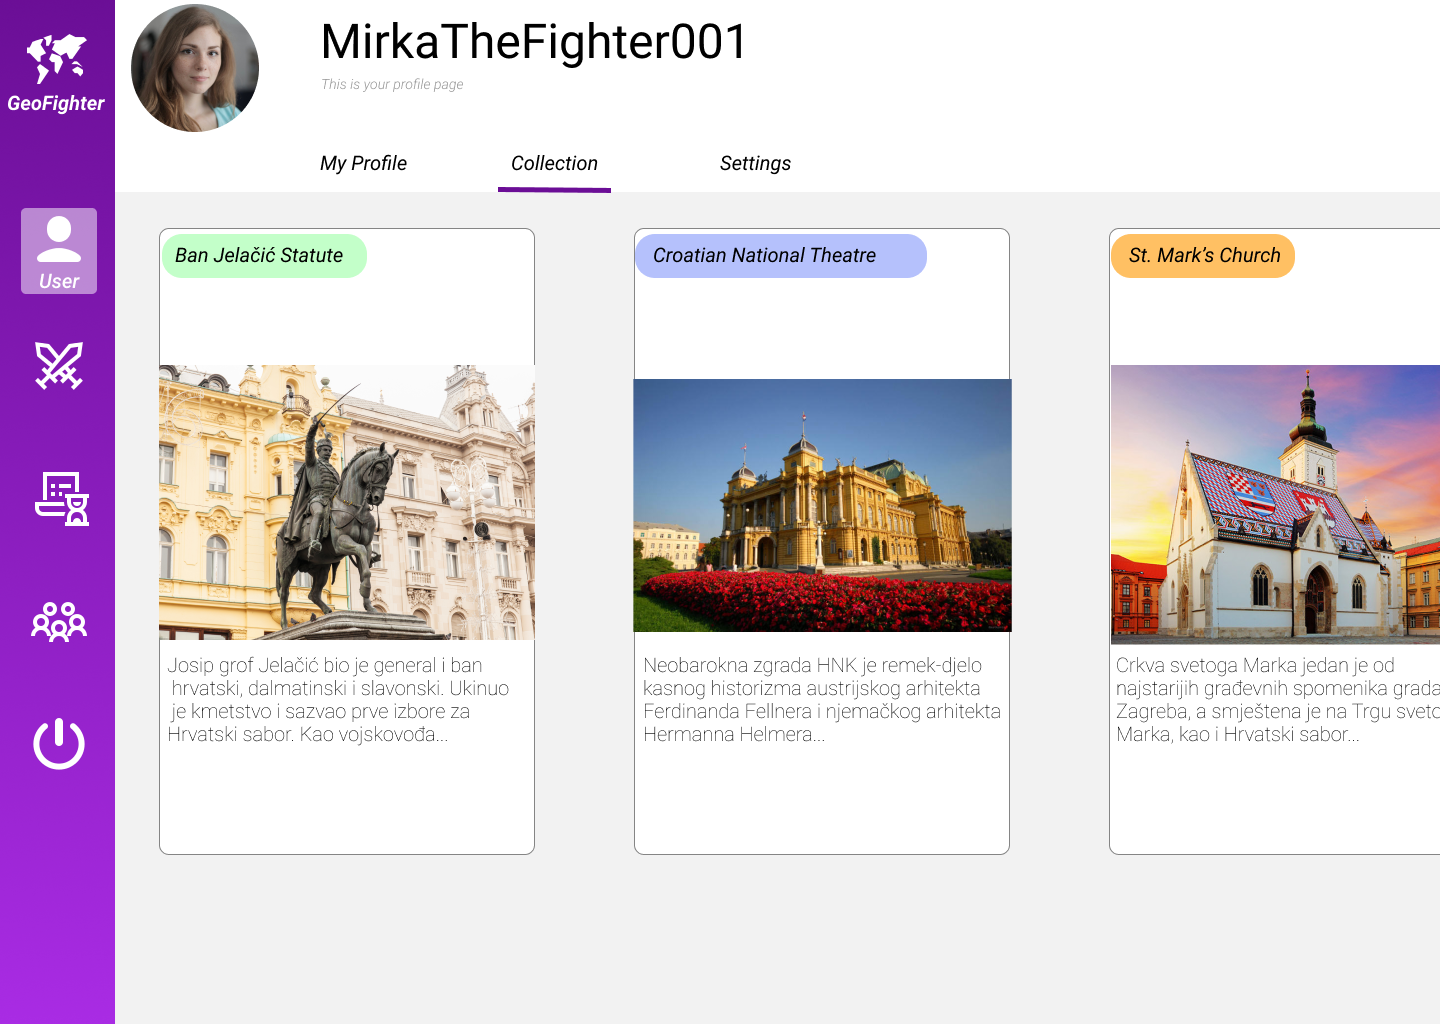
\includegraphics[scale=0.2]{slike/example} \\%veličina u odnosu na širinu linije
			\caption{WorkInProgress Primjer UI igrača}
			\label{fig:example} %label mora biti drugaciji za svaku sliku
		\end{figure}
		
		
		\textnormal{Igračima je dostupan pregled profila ostalih igrača, pregled vlastitog profila, pregled svih karata lokacija, poredak svih igrača prema elo sustavu, pregled igrača u blizini te mogućnosti započinjanja borbe ili prijave nove karte lokacije. Prilikom pregleda profila nekog igrača, prikazuju se sve karte koje je igrač ikad sakupio, rang na globalnoj ljestvici i statistike vezane uz zadnjih 10 borbi s drugim igračima. Istražujući svoju okolinu igrači sakupljaju lokacije tako da im dođu na dovoljnu udaljenost (3km). Lokacije se sakupljaju u obliku igraćih karata koje igrači koriste za međusobne bitke. Pritiskom na gumb za traženje borbe, igrač može poslati zahtjev za igru nekome od igrača koji su u blizini, ili prihvatiti zahtjev koji je dobio od nekog drugog igrača. Kada se dvoje igrača spare u borbu, otvaraju im se prozori za odabir karata za borbu iz vlastite kolekcije te nakon odabira borba kreće.}\\
		
		\textnormal{Borba se odvija matematičkim izračunom s obzirom na jačine odabranih karata. Svaka karta ima 3 atributa u vrijednosti 0-10 (0-najslabije, 10-najjače). Prije početka borbe igrači moraju odabrati 3 karte za borbu iz vlastite kolekcije. Nakon obavljenog izračuna s obzirom na jačine izabranih karata dobiva se povratna informacija o ishodu borbe. Na kraju se za svakog igrača dodjeljuje rating prema ELO rating sistemu koji se koristi i u šahu.}
		\textnormal{Nakon borbe, korištene karte dobivaju cooldown, odnosno ne mogu se koristiti slijedećih sat vremena nakon borbe, te se svakim novim korištenjem taj cooldown produljuje za još sat vremena, kako bi se igrače potaknulo na aktivan život i istraživanje te kako bi imali veću kolekciju i uvijek bili spremni za borbu.}\\
		
		\textnormal{Sučelje kartografa razlikuje se od sučelja igrača. Kartografu se prijave pokazuju na karti te ukoliko nije zadovoljan prijavom i/ili želi provjeriti danu lokaciju, sustav preko vanjskog servisa OSRM (Open source routing machine) dohvati rješenje problema trgovačkog putnika i kartografu put prikaže na karti. Nakon analize prijave, kartograf odlučuje hoće li prijavu odbiti ili prihvatiti. Također može prepraviti prijavu nakon provjere na terenu (promjena slike ili opisa) ili nakon uređivanja dodijeljenih vrijednosti atributa te ju zatim prihvatiti. Ukoliko je kartograf prihvatio prijavu, igraču se dodjeljuje igraća karta te lokacije.}\\
		
		\textnormal{Sučelje administratora sastoji se od svih funkcionalnosti sučelja igrača, kartografa te sučelja administratora. Administrator može pritiskom na gumb vidjeti popis svih registriranih igrača i kartografa, vidjeti i mijenjati njihove osobne podatke ili onemogućiti pristup nekome od korisnika. On jedini može brisati i uređivati postojeće lokacije tj. igraće karte.}\\
		
		
		\textnormal{Ovaj projekt potencijalno bi mogao koristiti korisnicima različitih generacija i interesa. Osim što će mlađe generacije izaći van na svjež zrak, baviti se tjelesnom aktivnošću i pritom igrati omiljenu im igricu, zajedno s prijateljima otkrivat će znamenitosti i ljepote Hrvatske te ponešto o svakoj naučiti.}
		
		\textnormal{Projekt će biti novi izazov za svakog gamera, malo drugačiji pogled na web-igre i razlog zbog kojeg će se mnoge korisnike redovno poticati na tjelesnu aktivnost. Promicat će se kulturna baština, širiti opće znanje stanovnika Republike Hrvatske, odlaziti u slabije pojećivana mjesta, a ovaj projekt mogao bi pozitivno pridonijeti i turizmu. Za turiste koji nisu u žurbi igra će biti savršen način za upoznavanje grada i istraživanje zanimljivih lokacija.}\\
		
		\textnormal{Također, aplikacija se ne mora nužno koristiti za borbu među igračima. Za avanturiste koje ne zanima borba i igranje igrice, aplikacija bi mogla služiti kao evidencija mjesta koja su posjetili. Dodavši neke prilagodbe kao mogućnost kontaktiranja i razmjenjivanja poruka među igračima, aplikacija  bi poprimila ugođaj društvene mreže na kojoj bi se ljudi mogli povezati s drugim avanturistima sličnih interesa. Razmjenjivanjem iskustava i preporuka, stvorila bi se mreža avanturista koji jedni drugima preporučaju zanimljive lokacije i postižu zadane si ciljeve.}
		
		\textnormal{Još jedna moguća  prilagodba aplikacije je za korištenje u edukativne svrhe. Prilikom namjernog ili nenamjernog posjeta nekoj obilježenoj lokaciji, osoba bi primila obavijest s informacijama o mjestu koje je posjetila, zajedno sa slikama i poveznicama za više informacija. Iste informacije mogla bi naknadno pogledati na svom korisničkom računu, na sučelju s posjećenim mjestima.}\\
		
		\textnormal{Ovisno o uspješnosti projektnog zadatka i dodatnim zahtjevima korisnika moguća je izrada iOS i Android aplikacija kako bi se poboljšale performanse na mobilnim uređajima. Također, integracijom s najpopularnijim društvenim mrežama bi se omogućilo igračima da podijele svoje uspjehe s prijateljima. Uvođenjem sustava achievementa (dostignuća) mogli bi se dodatno nagrađivati igrači. Mogli bi vidjeti koje achievemente još nisu osvojili i koji su koraci sve potrebni da ih osvoje. Korištenjem API-ova možemo nadopuniti listu lokacija, te ubrzati postupak njihovog dodavanja. Za vrijeme posebnih događaja kao što su Nova godina, Božić i slično mogli bi dodati posebne karte koje se samo tada, u kratkom roku, mogu sakupiti. Uvođenje posebnih lokacija za koje je potrebno više ljudi da se osvoje je također moguća nadogradnja. Najveća potencijalna nadogradnja je uvođenje AR (Augmented reality) sposobnosti kako bi igrači mogli oko sebe pomoću ugrađene kamere na mobilnom uređaju lakše pronaći sve moguće lokacije u svojoj blizini.}\\
		
		
		\textnormal{Najpoznatije postojeće slično rješenje je igra za ručne mobilne uređaje \textbf{Pokémon GO}. Pomoću GPS lokacije igrača oni se smještaju na virtualnu mapu koja emulira stvarni svijet, uz dodane lokacije gdje je moguća borba i sakupljanje Pokémona koji služe za borbu. Borbe se odvijaju pomoću jačine Pokémona, kao što će to biti slučaj s kartama u ovome projektu. Razlike u odnosu na ovaj projekt su to što je u igrici Pokémon GO omogućen prikaz mape po kojoj se igrač kreće analogno svom kretanju u stvarnosti. Također, za održavanje borbi u našem projektu će biti samo važni igrači koji su udaljeni 50 km od korisnika kako bi se pronašao suigrač, ali ne i sama lokacija korisnika kao što je to u Pokémon GO.    }
		
		\begin{figure}[H]
			\centering
			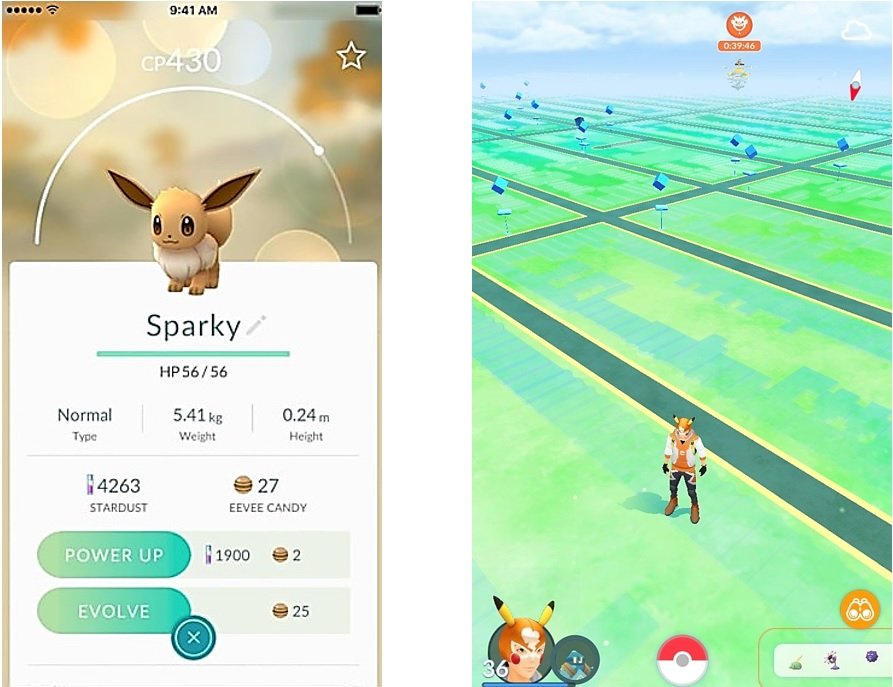
\includegraphics[scale=0.6]{slike/PokemonGO} \\%veličina u odnosu na širinu linije
			\caption{Prikaz kartice Pokémona i mape igrice Pokémon GO}
			\label{fig:PokemonGO} %label mora biti drugaciji za svaku sliku
		\end{figure}
	
		\textnormal{\textbf{Maguss} je mobilna igrica u kojoj su korisnici pomoću GPS-a smješteni na virtualnu mapu koja emulira stvarni svijet, ali uz dodatne lokacije na kojima je moguće sakupiti razna stvorenja, napitke i čarolije u obliku kartica. Ovaj projekt neće imati prikaz kretanja po mapi te će također postojati samo jedna vrsta stvari koju je moguće sakupiti, točnije kartica lokacije. Koncept duela sličan je borbama u ovome projektu jer se odvija karticama te suparnici ne moraju biti na identičnoj lokaciji, ali je različit po tome što dueli u igrici Maguss uključuju i dodatne zadatke kao što su iscrtavanje poteza. Također, u igrici Maguss jačina karata mijenja se brojem pobjeda što nije slučaj u našoj igrici. Za razliku od našeg projekta, kretanje u ovoj igrici osim pronalaska novih kartica djeluje i kao način punjenja energije igrača.}\\
		
		\begin{figure}[H]
			\centering
			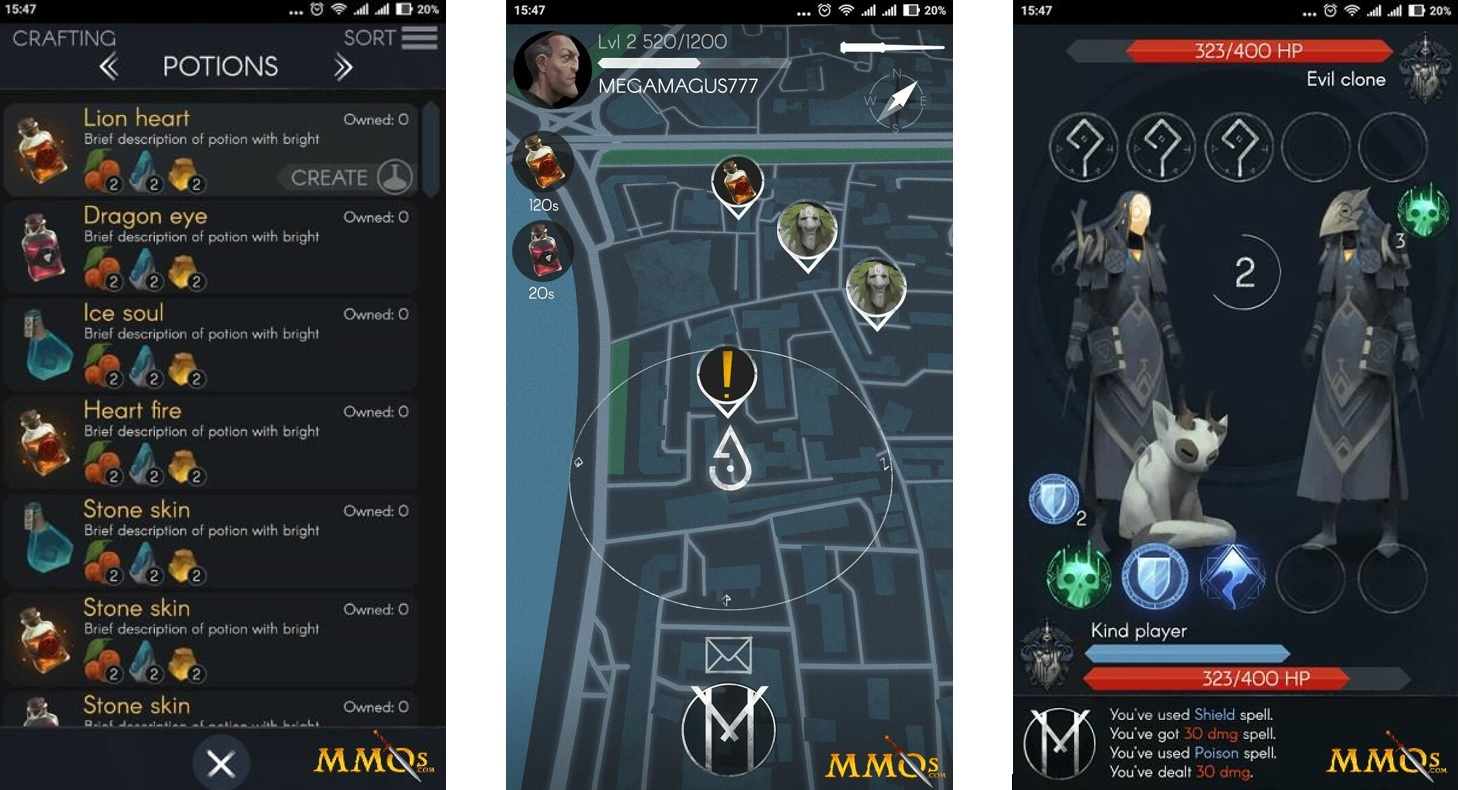
\includegraphics[scale=0.4]{slike/Maguss} \\%veličina u odnosu na širinu linije
			\caption{Prikaz sakupljenih kartica, mape i duela u igrici Maguss}
			\label{fig:Maguss} %label mora biti drugaciji za svaku sliku
		\end{figure}
	
		\textnormal{\textbf{Landlord Real Estate Tycoon} je mobilna igrica u kojoj se prema GPS lokaciji igrača prikazuju stvarne lokacije njemu u blizini u obliku kartica lokacija koje zatim može kupovati. To je prva razlika u odnosu na ovaj projekt, jer će u ovome projektu na jednoj lokaciji biti dostupna samo jedna kartica lokacije te za dobivanje kartice neće biti potrebna nikakva monetarna vrijednost kao što je to u igrici Landlord Real Estate Tycoon. Također se mogu davati ponude za kartice drugih igrača, a cilj igre je istraživanjem, kupovanjem i preprodavanjem povećati svoju monetarnu vrijednost. U igrici Real Estate Tycoon nema ničega sličnog borbama u ovome projektu. Također, u ovome projektu neće biti moguća razmjena kartica između igrača. }
		
		\begin{figure}[H]
			\centering
			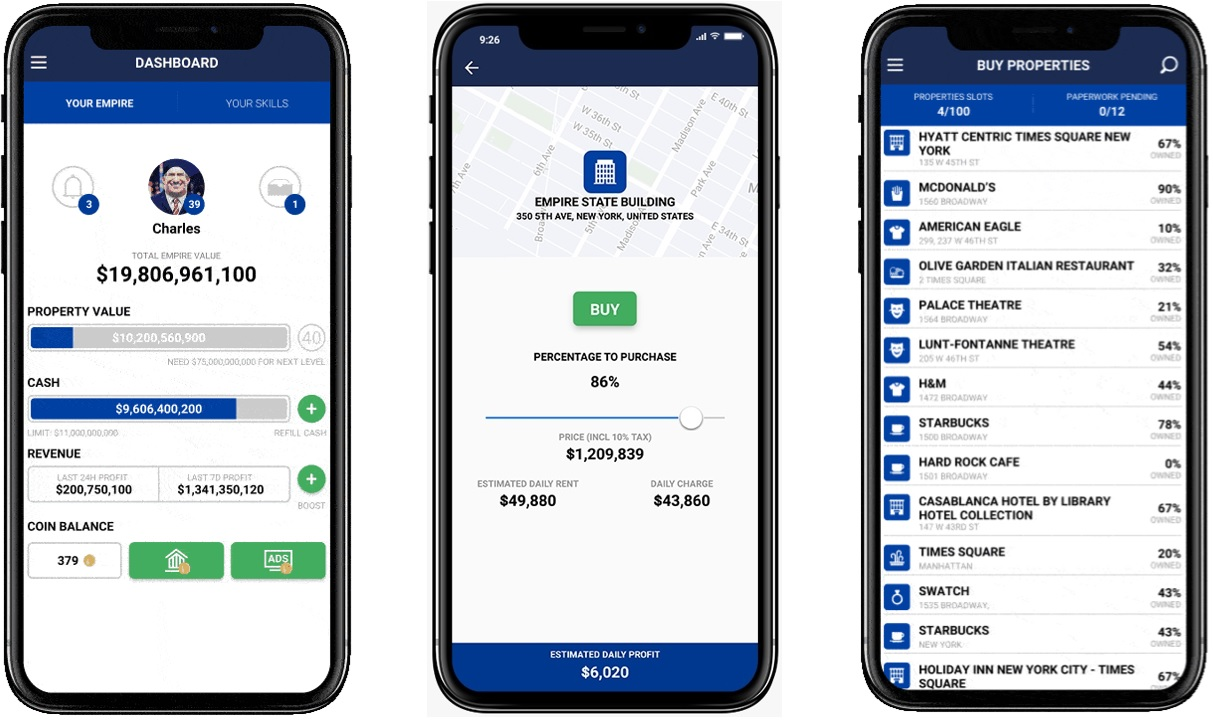
\includegraphics[scale=0.6]{slike/Landlord} \\%veličina u odnosu na širinu linije
			\caption{Prikaz profila igrača, kartice lokacije i dostupnih lokacija u igrici Landlord Real Estate Tycoon}
			\label{fig:Landlord} %label mora biti drugaciji za svaku sliku
		\end{figure}
	
		\textnormal{Još jedna mobilna igrica slična ovome projektu je \textbf{Ghostbusters World}. Igrači trebaju doći na stvarnu lokaciju koja je pomoću GPS-a u igrici označena kao mjesto gdje postoje duhovi. Na tim lokacijama nakon odigrane mini-igre mogu postaviti zamku te time dobiti nekog od duhova u obliku kartice. Također, u igrici Ghostbusters World omogućen je prikaz duhova u stvarnom svijetu pomoću kamere te prikaz putovanja igrača kroz virtualan svijet, što u ovome projektu neće biti omogućeno. Također su omogućeni dueli igrača gdje se bore sakupljenim karticama duhova, no izbor suparnika ne ovisi o međusobnoj udaljenosti igrača kao što će biti slučaj u ovome projektu, već se igrači smještaju u tzv. Arene, ovisno o napretku u igrici, unutar kojih se mogu boriti.}
		
		\begin{figure}[H]
			\centering
			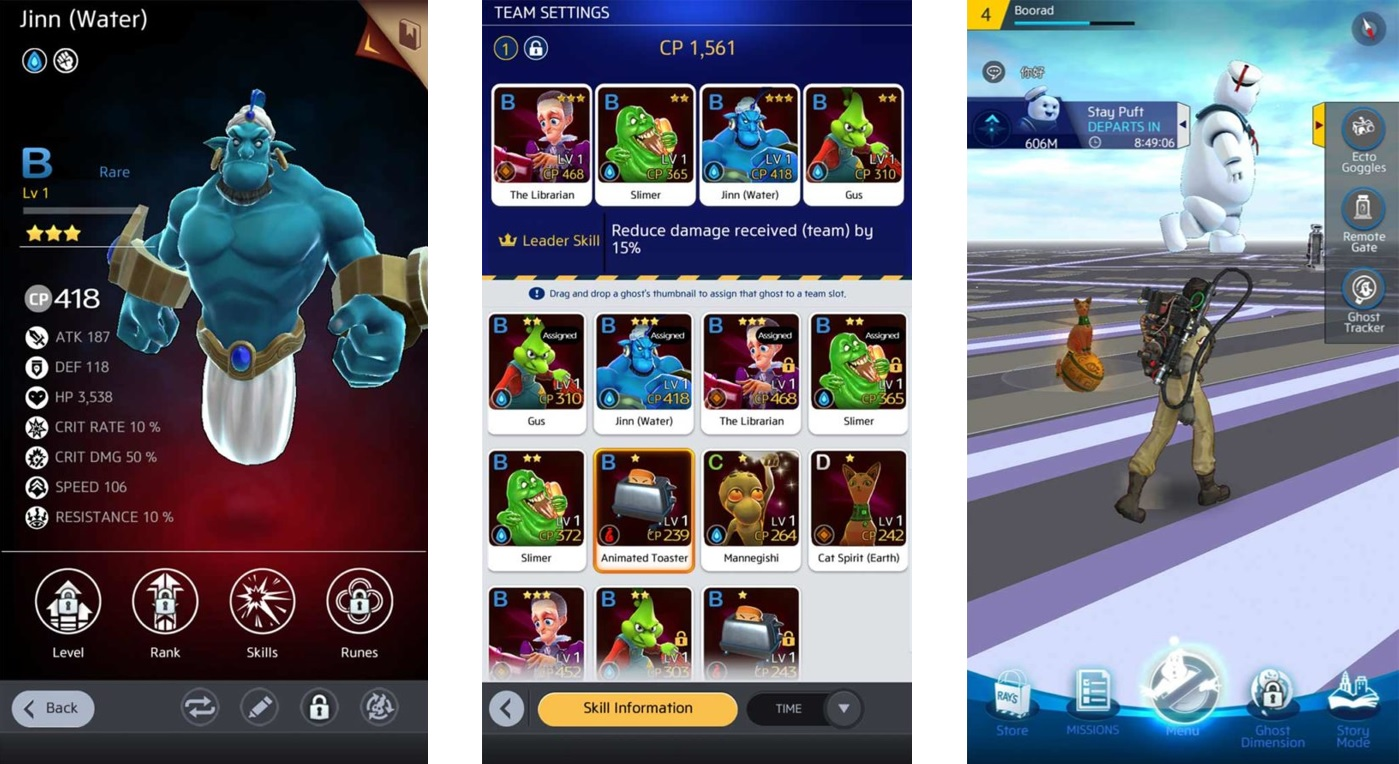
\includegraphics[scale=0.6]{slike/Ghostbusters} \\%veličina u odnosu na širinu linije
			\caption{Prikaz igrače kartice, sakupljenih kartica i igrača virtualnom svijetu igrice Ghostbusters World}
			\label{fig:Ghostbusters} %label mora biti drugaciji za svaku sliku
		\end{figure}	
		
		\eject
		
		
	\chapter{Specifikacija programske potpore}
		
	\section{Funkcionalni zahtjevi}
			
			\textbf{\textit{dio 1. revizije}}\\
			
			\textit{Navesti \textbf{dionike} koji imaju \textbf{interes u ovom sustavu} ili  \textbf{su nositelji odgovornosti}. To su prije svega korisnici, ali i administratori sustava, naručitelji, razvojni tim.}\\
				
			\textit{Navesti \textbf{aktore} koji izravno \textbf{koriste} ili \textbf{komuniciraju sa sustavom}. Oni mogu imati inicijatorsku ulogu, tj. započinju određene procese u sustavu ili samo sudioničku ulogu, tj. obavljaju određeni posao. Za svakog aktora navesti funkcionalne zahtjeve koji se na njega odnose.}\\
			
			
			\noindent \textbf{Dionici:}
			
			\begin{packed_enum}
				
				\item Razvojni tim
				\item Igrači				
				\item Kartografi
				\item Admin
				
			\end{packed_enum}
			
			\noindent \textbf{Aktori i njihovi funkcionalni zahtjevi:}
			
			
			\begin{packed_enum}
				\item  \underbar{Neregistrirani korisnik (inicijator) može:}
				
				\begin{packed_enum}
					
					\item se registrirati u sustav kao:
					\begin{packed_enum}
						
						\item  igrač (stvaranje korisničkog računa, potrebni sljedeći podaci: korisničko ime, lozinka, e-mail adresa, fotografija)
						\item  kartograf (stvaranje korisničkog računa, potrebni sljedeći podaci: IBAN računa za uplatu, fotografija osobne iskaznice)
				
					\end{packed_enum}
					
				\end{packed_enum}
			
				\item  \underbar{Igrač (inicijator) može:}
				
				\begin{packed_enum}
					
					\item se prijaviti u sustav koristeći email i lozinku
					\item se odjaviti iz sustava
					\item pregledati vlastiti profil
					\begin{packed_enum}
						\item pristupiti prikazu svih sakupljenih karti
						\item pristupiti prikazu statistike 10 zadnjih odigranih borbi
					\end{packed_enum}
				\item pregledati profil drugog igrača
				\begin{packed_enum}
					\item pristupiti prikazu svih sakupljenih karti
					\item pristupiti prikazu statistike 10 zadnjih odigranih borbi
				\end{packed_enum}
			\item pregledati detalje pojedinačne karte iz kolekcije
			\item pregledati popis igrača u blizini
			\item pristupiti borbi kroz nasumičnu tražilicu
			\item se boriti u kartaškom dvoboju protiv drugog igrača
			\begin{packed_enum}
				\item odabrati karte za borbu iz svoje kolekcije sakupljenih karata
				\item odigrati kartaški dvoboj
			\end{packed_enum}
		\item prijaviti novu lokaciju
		\item dobiti novu kartu ako ju je igrač prijavio te je ona odobrena bez izmjena
		\item pristupiti pregledu rang ljestvice svih igrača
					
				\end{packed_enum}
			\item  \underbar{Kartograf (inicijator) može:}
			
			\begin{packed_enum}
				\item se prijaviti u sustav preko broja osobne iskaznice
				\item se odjaviti iz sustava
				\item pristupiti prikazu svih prijava:
				\begin{packed_enum}
					\item prihvatiti lokaciju iz prijave
					\item odbiti lokaciju iz prijave
					\item može izmijeniti prijavu te zatim lokaciju prihvatiti
					\item može odabrati opciju da je potrebna potvrda s terena, te ga sustav na mapi vodi najkraćim putem od vlastite lokacije do prijavljene lokacije
				\end{packed_enum}
			\end{packed_enum}
		\item  \underbar{Administrator (inicijator) uz mogućnosti kartografa i igrača može:}
		\begin{packed_enum}
			\item pristupiti pregledu popisa svih korisnika
			\begin{packed_enum}
				\item brisati korisnike s popisa, odnosno ukloniti korisnike iz igre
				\item uređivati osobne podatke svih korisnika
				\item isključiti igrače privremeno iz igre
			\end{packed_enum}
		\item pristupiti pregledu svih lokacija (karti) u igri
		\begin{packed_enum}
			\item uređivati postojeće lokacije (karte)
			\item brisati postojeće lokacije (karte)
		\end{packed_enum}
	\item pristupiti pregledu prijava kartografa
	\begin{packed_enum}
		\item prihvatiti prijavu
		 \item odbiti prijavu
	\end{packed_enum}
		\end{packed_enum}
	\item  \underbar{Baza podataka (sudionik):}
	\begin{packed_enum}
		\item pohranjuje sve podatke o svim korisnicima, njihovim kolekcijama i njihovim ovlastima
		\item pohranjuje sve podatke o postojećim lokacijama i prijavama lokacija
	\end{packed_enum}
\item  \underbar{OSRM (sudionik) :}
		\begin{packed_enum}
			\item omogućava pronalazak najkraćeg puta dvije lokacije na mapi
		\end{packed_enum}
			\end{packed_enum}
			
			\eject 
			
			
				
			\subsection{Obrasci uporabe}
				
				\textbf{\textit{dio 1. revizije}}
				
				\subsubsection{Opis obrazaca uporabe}
					\textit{Funkcionalne zahtjeve razraditi u obliku obrazaca uporabe. Svaki obrazac je potrebno razraditi prema donjem predlošku. Ukoliko u nekom koraku može doći do odstupanja, potrebno je to odstupanje opisati i po mogućnosti ponuditi rješenje kojim bi se tijek obrasca vratio na osnovni tijek.}\\
				
				\noindent \underbar{\textbf{UC1 -Registracija}}
				\begin{packed_item}
					
					\item \textbf{Glavni sudionik: }Neregistrirani korisnik
					\item  \textbf{Cilj:} Stvoriti korisnički račun za pristup sustavu
					\item  \textbf{Sudionici:} Baza podataka
					\item  \textbf{Preduvjet:} -
					\item  \textbf{Opis osnovnog tijeka:}
					
					\item Korisnik odabire opciju za registraciju.
					\item Korisnik unosi potrebne korisničke podatke.
					\item Korisnik prima e-mail za potvrdu registracije.
					\item Potvrdom e-maila korisnik prima obavijest o uspješnoj registraciji.
					\item[] \begin{packed_item}
						
						\item[2.a] Odabir već zauzetog korisničkog imena i/ili e-maila, unos korisničkog podatka u nedozvoljenom formatu ili neispravnoga e-maila.
						\item[] \begin{packed_enum}
							
							\item Sustav obavještava korisnika o neuspjelom upisu i vraća ga na stranicu za registraciju.
							\item Korisnik mijenja potrebne podatke te završava unos ili odustaje od registracije.
							
						\end{packed_enum}
						
					\end{packed_item}
				\end{packed_item}
				\noindent \underbar{\textbf{UC1.2 -Registracija kartografa}}
				\begin{packed_item}
					
					\item \textbf{Glavni sudionik: }Neregistrirani korisnik
					\item  \textbf{Cilj:} Stvoriti korisnički račun za pristup sustavu kao kartograf
					\item  \textbf{Sudionici:} Baza podataka
					\item  \textbf{Preduvjet:} -
					\item  \textbf{Opis osnovnog tijeka:}
					
					\item[] \begin{packed_enum}
						
						\item Korisnik odabire opciju za registraciju.
						\item Korisnik unosi potrebne korisničke podatke.
					\end{packed_enum}
					
					\item  \textbf{Opis mogućih odstupanja:}
					
					\item[] \begin{packed_item}
						
						\item[2.a] Odbijenica od strane administratora
						\item[] \begin{packed_enum}
							
							\item Prihvatiti odbijenicu i pokusati se prijaviti drugi put
							
						\end{packed_enum}
						
					\end{packed_item}
				\end{packed_item}
				\noindent \underbar{\textbf{UC2 -Prijava}}
				\begin{packed_item}
					
					\item \textbf{Glavni sudionik: }Registrirani korisnik
					\item  \textbf{Cilj:} Dobiti pristup korisničkom sučelju
					\item  \textbf{Sudionici:} Baza podataka
					\item  \textbf{Preduvjet:} Registracija
					\item  \textbf{Opis osnovnog tijeka:}
					
					\item[] \begin{packed_enum}
						
						\item Unos emaila i lozinke.
						\item Potvrda o ispravnosti unesenih podataka.
						\item Pristup korisničkim funkcijama.
					\end{packed_enum}
					
					\item  \textbf{Opis mogućih odstupanja:}
					
					\item[] \begin{packed_item}
						
						\item[2.a] Neispravan email ili lozinka
						\item[] \begin{packed_enum}
							
							\item  Sustav obavještava korisnika o neuspješnoj prijavi. Korisnik pokušava ponovno.
							\item Sustav obavještava korisnika o neuspješnoj prijavi. Korisnik odustaje.
							
						\end{packed_enum}
						
					\end{packed_item}
				\end{packed_item}
				\noindent \underbar{\textbf{UC3 -Odjava iz sustava}}
				\begin{packed_item}
					
					\item \textbf{Glavni sudionik: }Registrirani korisnik
					\item  \textbf{Cilj:} Završetak korištenja korisničkog sučelja.
					\item  \textbf{Sudionici:} Baza podataka
					\item  \textbf{Preduvjet:} Prijava
					\item  \textbf{Opis osnovnog tijeka:}
					
					\item[] \begin{packed_enum}
						
						\item Korisnik odabire opciju za odjavu.
						\item Sustav odjavljuje korisnika i vraća ga na početnu stranicu.
					\end{packed_enum}
					
				\end{packed_item}
				
				\noindent \underbar{\textbf{UC4 - Pregled vlastitog profila}}
				\begin{packed_item}
					
					\item \textbf{Glavni sudionik: }Registrirani korisnik
					\item  \textbf{Cilj:} Pregled vlastitog profila
					\item  \textbf{Sudionici:} Baza podataka
					\item  \textbf{Preduvjet:} Prijava
					\item  \textbf{Opis osnovnog tijeka:}
					
					\item[] \begin{packed_enum}
						
						\item Korisnik odabire opciju za pregled vlastitog profila.
						\item Aplikacija prikazuje osobne podatke, vlastiti rang i statistiku zadnjih 10 borbi.
					\end{packed_enum}
				\end{packed_item}
				
				\noindent \underbar{\textbf{UC4.1 -Pregled svih sakupljenih karata}}
				\begin{packed_item}
					
					\item \textbf{Glavni sudionik: }Registrirani korisnik
					\item  \textbf{Cilj:} Pregled svih sakupljenih karata
					\item  \textbf{Sudionici:} Baza podataka
					\item  \textbf{Preduvjet:} Pregled vlastitog ili tuđeg profila
					\item  \textbf{Opis osnovnog tijeka:}
					
					\item[] \begin{packed_enum}
						
						\item Korisnik odlazi na svoj ili tuđi profil.
						\item Odabire opciju pregleda kolekcije karata.
						\item Aplikacija prikazuje sve karte koje taj profil ima u svojoj kolekciji.
					\end{packed_enum}
				\end{packed_item}
				
				\noindent \underbar{\textbf{UC5 -Pregled profila drugog igrača}}
				\begin{packed_item}
					
					\item \textbf{Glavni sudionik: }Registrirani korisnik
					\item  \textbf{Cilj:} Pregled podataka drugog igrača
					\item  \textbf{Sudionici:} Baza podataka
					\item  \textbf{Preduvjet:} Pregled igrača u blizini ili pregled rang ljestvice
					\item  \textbf{Opis osnovnog tijeka:}
					
					\item[] \begin{packed_enum}
						
						\item Korisnik odabire igrača s popisa čiji profil želi otvoriti.
						\item Prikazuju se detalji drugog igrača: ime, rang, statistika zadnjih 10 borbi te gumb za kolekciju.
					\end{packed_enum}
				\end{packed_item}
				
				\noindent \underbar{\textbf{UC6 -Pregled pojedinačne karte}}
				\begin{packed_item}
					
					\item \textbf{Glavni sudionik: }Registrirani korisnik
					\item  \textbf{Cilj:} Pregled kartice lokacije
					\item  \textbf{Sudionici:} Baza podataka
					\item  \textbf{Preduvjet:} Pregled svih sakupljenih karata
					\item  \textbf{Opis osnovnog tijeka:}
					
					\item[] \begin{packed_enum}
						
						\item Korisnik odabire jednu od karata.
						\item Aplikacija prikazuje sve dostupne podatke o karti lokacije.
					\end{packed_enum}
				\end{packed_item}
				
				\noindent \underbar{\textbf{UC7 -Pregled igrača u blizini}}
				\begin{packed_item}
					
					\item \textbf{Glavni sudionik: }Registrirani korisnik
					\item  \textbf{Cilj:} Pregled igrača unutar radijusa od 50 km
					\item  \textbf{Sudionici:} Baza podataka
					\item  \textbf{Preduvjet:} Prijava
					\item  \textbf{Opis osnovnog tijeka:}
					
					\item[] \begin{packed_enum}
						
						\item Korisnik odabire opciju za pregled igrača u blizini.
						\item Aplikacija prikazuje popis svih igrača unutar radijusa od 50 km.
					\end{packed_enum}
				\end{packed_item}
				
				\noindent \underbar{\textbf{UC8 -Borba}}
				\begin{packed_item}
					
					\item \textbf{Glavni sudionik: }Registrirani korisnik
					\item  \textbf{Cilj:} Odigrati borbu
					\item  \textbf{Sudionici:} Baza podataka, suigrač
					\item  \textbf{Preduvjet:} Traženje borbe
					\item  \textbf{Opis osnovnog tijeka:}
					
					\item[] \begin{packed_enum}
						
						\item Korisnik odabire opciju za pronalazak suparnika, sustav uparuje.
						\item Prikaže se kolekcija karata.
						\item Korisnik izabire karte s kojima će igrati.
						\item Korisnik odabire opciju "Potvrdi karte", prikazuje se prozor za borbu.
						\item Baca se novčić da se vidi koji će igrač imati prvi potez.
						\item Igrači su naizmjence na potezu, na vlastitom potezu odabiru kartu koju žele odigrati i atribut koji se koristi u borbi.
						\item Kada su obje karte bačene ona s jačim atributom pobjeđuje rundu
						\item Nakon što su kartice potrošene(5), igra završava.
					\end{packed_enum}
					
					\item  \textbf{Opis mogućih odstupanja:}
					
					\item[] \begin{packed_item}
						
						\item[1.a] Igrač odustane ili izgubi vezu
						\item[] \begin{packed_enum}
							
							\item  Sustav čeka korisnika 30 sekundi kako bi se ponovno povezao u sustav, a ako se to ne dogodi, drugom igraču je dodijeljena pobjeda.
							
						\end{packed_enum}
						\item[2.a] Igrač nema dovoljno karata za borbu
						\item[] \begin{packed_enum}
							
							\item  Prilikom pritiska na gumb "Traži borbu" sustav igraču javlja kako nema dovoljno karata za početak borbe (ili ih nema dovoljno ili su na cooldownu pa nisu trenutno dostupne). Sustav mu predlaže da pođe u istraživanje kako bi sakupio više karata i uvijek bio spreman na borbu.
							
						\end{packed_enum}
						
					\end{packed_item}
				\end{packed_item}
				
				\noindent \underbar{\textbf{UC8.1 -Odabir karata za borbu}}
				\begin{packed_item}
					
					\item \textbf{Glavni sudionik: }Registrirani korisnik.
					\item  \textbf{Cilj:} Izbor karata za borbu.
					\item  \textbf{Sudionici:} Baza podataka.
					\item  \textbf{Preduvjet:} Pronađen je suigrač.
					\item  \textbf{Opis osnovnog tijeka:}
					
					\item[] \begin{packed_enum}
						
						\item Aplikacija prikazuje sve sakupljene karte korisnika.
						\item Korisnik odabire 5 karata za borbu. 
						\item Korisnik odabire opciju za početak borbe.
					\end{packed_enum}
					
					\item  \textbf{Opis mogućih odstupanja:}
					
					\item[] \begin{packed_item}
						
						\item[2.a] Pokušaj odabira karte koja je na cooldownu
						\item[] \begin{packed_enum}
							
							\item  sustav javlja da je karta na cooldownu te da je potrebno odabrati drugu kartu za borbu.
							
						\end{packed_enum}
						
					\end{packed_item}
				\end{packed_item}
				
				\noindent \underbar{\textbf{UC8.2 -Kraj borbe}}
				\begin{packed_item}
					
					\item \textbf{Glavni sudionik: }Registrirani korisnik
					\item  \textbf{Cilj:} Završetak borbe
					\item  \textbf{Sudionici:} Baza podataka
					\item  \textbf{Preduvjet:} Borba je odigrana
					\item  \textbf{Opis osnovnog tijeka:}
					
					\item[] \begin{packed_enum}
						
						\item Aplikacija prikaže poruku ovisno o pobjedi ili porazu.
						\item Statistika oba suigrača se osvježi u bazi podataka.
						\item Kartama koje su korištene smanjuju se 	bodovi.
						\item Sustav vraća korisnika na početnu stranicu.
					\end{packed_enum}
				\end{packed_item}
				
				\noindent \underbar{\textbf{UC9 -Prijava nove lokacije}}
				\begin{packed_item}
					
					\item \textbf{Glavni sudionik: }Registrirani korisnik
					\item  \textbf{Cilj:} Dodavanje nove kartice lokacije u igru
					\item  \textbf{Sudionici:} Baza podataka, kartograf
					\item  \textbf{Preduvjet:} Dovoljno iskustvo u igri
					\item  \textbf{Opis osnovnog tijeka:}
					
					\item[] \begin{packed_enum}
						
						\item Korisnik odabire opciju za prijavu nove lokacije.
						\item Korisnik unosi potrebne podatke.
						\item Sustav šalje prijavu kartografu.
					\end{packed_enum}
					\item  \textbf{Opis mogućih odstupanja:}
					
					\item[] \begin{packed_item}
						
						\item[1.a] Pokušaj slanja nepotpune prijave
						\item[] \begin{packed_enum}
							
							\item  Sustav javlja da je prijava nepotpuna, igrač će odustati od prijave lokacije. 
							\item  Sustav javlja da je prijava nepotpuna, igrač će ispuniti tražena polja.
							
						\end{packed_enum}
						
					\end{packed_item}
				\end{packed_item}
				
				\noindent \underbar{\textbf{UC9.1 - Osvajanje nove karte zbog prijave lokacije}}
				\begin{packed_item}
					
					\item \textbf{Glavni sudionik: }Registrirani korisnik
					\item  \textbf{Cilj:} Osvajanje lokacije(karte)
					\item  \textbf{Sudionici:} Baza podataka, kartograf
					\item  \textbf{Preduvjet:} Prihvaćena prijava lokacije bez izmjena
					\item  \textbf{Opis osnovnog tijeka:}
					
					\item[] \begin{packed_enum}
						
						\item Korisnikova prijava je prihvaćena bez potrebnih daljnjih izmjena.
						\item Korisnik dobiva obavijest da mu je dodijeljena nova karta.
						\item Nova karta(lokacija) se dodaje u kolekciju korisnika.
					\end{packed_enum}
				\end{packed_item}
				
				\noindent \underbar{\textbf{UC10 - Pregled rang ljestvice}}
				\begin{packed_item}
					
					\item \textbf{Glavni sudionik: }Registrirani korisnik
					\item  \textbf{Cilj:} Pregled rang ljestvice svih igrača
					\item  \textbf{Sudionici:} Baza podataka
					\item  \textbf{Preduvjet:} -
					\item  \textbf{Opis osnovnog tijeka:}
					
					\item[] \begin{packed_enum}
						
						\item Korisnik odabire opciju prikaza rang ljestvice
						\item Korisniku se otvara rang ljestvica na kojoj može vidjeti sve igrače poredane po rangu
					\end{packed_enum}
				\end{packed_item}
					
				
				\noindent \underbar{\textbf{UC11 - Pregled popisa korisnika}}
				\begin{packed_item}
					
					\item \textbf{Glavni sudionik: }Administrator
					\item  \textbf{Cilj:} Pregled popisa korisnika
					\item  \textbf{Sudionici:} Baza podataka
					\item  \textbf{Preduvjet:} Korisnik je prijavljen kao administrator
					\item  \textbf{Opis osnovnog tijeka:}
					
					\item[] \begin{packed_enum}
						
						\item Administrator klikom na opciju za pregled registriranih korisnika šalje upit bazi podataka.
						\item Baza podataka vraća popis registriranih korisnika.
						\item Popis korisnika se administratoru prikazuje u web sučelju.
					\end{packed_enum}
					
				\end{packed_item}
			
				\noindent \underbar{\textbf{UC11.1 - Brisanje korisnika s popisa}}
				\begin{packed_item}
					
					\item \textbf{Glavni sudionik: }Administrator
					\item  \textbf{Cilj:} Izbrisati korisnika s popisa iz baze podataka
					\item  \textbf{Sudionici:} Baza podataka
					\item  \textbf{Preduvjet:} Korisnik je prijavljen kao administrator
					\item  \textbf{Opis osnovnog tijeka:}
					
					\item[] \begin{packed_enum}
						
						\item Administrator odabire opciju za pregled registriranih korisnika.
						\item Popis korisnika se administratoru prikazuje u web sučelju.
						\item Pored imena korisnika administrator odabire opciju za brisanje korisnika.
						\item Korisnik se briše iz baze podataka.
						\item Ažurira se popis korisnika u web sučelju.
					\end{packed_enum}
					
				\end{packed_item}
			
				\noindent \underbar{\textbf{UC11.2 - Uređivanje osobnih podataka korisnika}}
				\begin{packed_item}
					
					\item \textbf{Glavni sudionik: }Administrator
					\item  \textbf{Cilj:} Urediti osobne podatke korisnika
					\item  \textbf{Sudionici:} Baza podataka
					\item  \textbf{Preduvjet:} Korisnik je prijavljen kao administrator
					\item  \textbf{Opis osnovnog tijeka:}
					
					\item[] \begin{packed_enum}
						
						\item Administrator odabire opciju za pregled registriranih korisnika.
						\item Popis korisnika se administratoru prikazuje u web sučelju.
						\item Administrator klikom na ime korisnika šalje upit bazi podataka.
						\item Podaci o korisniku se prikazuju administratoru.
						\item Administrator mijenja korisničke podatke i odabire opciju za spremanje.
						\item Aplikacija šalje nove korisničke podatke bazi podataka.
					\end{packed_enum}
					
					\item  \textbf{Opis mogućih odstupanja:}
					
					\item[] \begin{packed_item}
						
						\item[3.a] Drugi administrator je u međuvremenu izbrisao korisnika
						\item[] \begin{packed_enum}
							
							\item Administratoru se ispisuje poruka da taj korisnik više ne postoji.
							
						\end{packed_enum}
						\item[6.a] Drugi administrator je u međuvremenu izbrisao korisnika
						\item[] \begin{packed_enum}
							
							\item Administratoru se ispisuje poruka da taj korisnik više ne postoji.
							
						\end{packed_enum}
						
					\end{packed_item}
				\end{packed_item}
				
				\noindent \underbar{\textbf{UC11.3 - Isključivanje igrača iz igre}}
				\begin{packed_item}
					
					\item \textbf{Glavni sudionik: }Administrator
					\item  \textbf{Cilj:} Isključiti igrača iz igre trajno ili privremeno
					\item  \textbf{Sudionici:} Baza podataka
					\item  \textbf{Preduvjet:} Korisnik je prijavljen kao administrator
					\item  \textbf{Opis osnovnog tijeka:}
					
					\item[] \begin{packed_enum}
						
						\item Administrator odabire opciju za pregled registriranih korisnika.
						\item Popis korisnika se administratoru prikazuje u web sučelju.
						\item Pored imena korisnika administrator odabire opciju za isključenje korisnika.
						\item Administratoru se prikazuje obrazac u kojem treba odabrati opciju za trajno ili privremeno isključenje uz navedeno vrijeme.
						\item Administrator potvrđuje odabir.
						\item Aplikacija zabilježi isključenog korisnika u bazi podataka.
					\end{packed_enum}
					
					\item  \textbf{Opis mogućih odstupanja:}
					
					\item[] \begin{packed_item}
						
						\item[3.a] Drugi administrator je u međuvremenu izbrisao korisnika
						\item[] \begin{packed_enum}
							
							\item Administratoru se ispisuje poruka da taj korisnik više ne postoji.
							
						\end{packed_enum}
						\item[5.a] Drugi administrator je u međuvremenu izbrisao korisnika
						\item[] \begin{packed_enum}
							
							\item Podaci o isključenom korisniku se ne bilježe u bazi podataka.
							\item Administratoru se ispisuje poruka da taj korisnik više ne postoji.
							
						\end{packed_enum}
						
					\end{packed_item}
				\end{packed_item}
				
				\noindent \underbar{\textbf{UC12 - Pregled popisa lokacija}}
				\begin{packed_item}
					
					\item \textbf{Glavni sudionik: }Administrator
					\item  \textbf{Cilj:} Pregled popisa lokacija igraćih karata
					\item  \textbf{Sudionici:} Baza podataka
					\item  \textbf{Preduvjet:} Korisnik je prijavljen kao administrator
					\item  \textbf{Opis osnovnog tijeka:}
					
					\item[] \begin{packed_enum}
						
						\item Administrator klikom na opciju za pregled lokacija šalje upit bazi podataka.
						\item Baza podataka vraća popis lokacija na kojima su karte.
						\item Popis lokacija se administratoru prikazuje u web sučelju.
					\end{packed_enum}
				\end{packed_item}
				
				\noindent \underbar{\textbf{UC12.1 - Uređivanje podataka lokacije}}
				\begin{packed_item}
					
					\item \textbf{Glavni sudionik: }Administrator
					\item  \textbf{Cilj:} Urediti podatke o lokaciji karte
					\item  \textbf{Sudionici:} Baza podataka
					\item  \textbf{Preduvjet:} Korisnik je prijavljen kao administrator
					\item  \textbf{Opis osnovnog tijeka:}
					
					\item[] \begin{packed_enum}
						
						\item Administrator odabire opciju za pregled lokacija.
						\item Popis lokacija se administratoru prikazuje u web sučelju.
						\item Administrator klikom na ime lokacije šalje upit bazi podataka.
						\item Podaci o lokaciji se prikazuju administratoru.
						\item Administrator mijenja podatke o lokaciji i odabire opciju za spremanje.
						\item Aplikacija šalje nove podatke o lokaciji bazi podataka.
					\end{packed_enum}
					
					\item  \textbf{Opis mogućih odstupanja:}
					
					\item[] \begin{packed_item}
						
						\item[3.a] Drugi administrator je u međuvremenu izbrisao lokaciju
						\item[] \begin{packed_enum}
							
							\item Administratoru se ispisuje poruka da ta lokacija više ne postoji.
							
						\end{packed_enum}
						\item[6.a] Drugi administrator je u međuvremenu izbrisao lokaciju
						\item[] \begin{packed_enum}
							
							\item Administratoru se ispisuje poruka da ta lokacija više ne postoji.
							
						\end{packed_enum}
						
					\end{packed_item}
				\end{packed_item}
				
				\noindent \underbar{\textbf{UC12.2 - Brisanje lokacije s popisa}}
				\begin{packed_item}
					
					\item \textbf{Glavni sudionik: }Administrator
					\item  \textbf{Cilj:} Izbrisati lokaciju s popisa iz baze podataka
					\item  \textbf{Sudionici:} Baza podataka
					\item  \textbf{Preduvjet:} Korisnik je prijavljen kao administrator
					\item  \textbf{Opis osnovnog tijeka:}
					
					\item[] \begin{packed_enum}
						
						\item Administrator odabire opciju za pregled lokacija.
						\item Popis lokacija se administratoru prikazuje u web sučelju.
						\item Pored imena lokacije administrator odabire opciju za brisanje lokacije.
						\item Lokacija se briše iz baze podataka.
						\item Ažurira se popis lokacija u web sučelju.
					\end{packed_enum}
				\end{packed_item}
				
				\noindent \underbar{\textbf{UC13 - Pregled prijava kartografa}}
				\begin{packed_item}
					
					\item \textbf{Glavni sudionik: }Administrator
					\item  \textbf{Cilj:} Pregledati popis prijava za ulogu kartografa
					\item  \textbf{Sudionici:} Baza podataka
					\item  \textbf{Preduvjet:} Korisnik je prijavljen kao administrator
					\item  \textbf{Opis osnovnog tijeka:}
					
					\item[] \begin{packed_enum}
						
						\item Administrator klikom na opciju za pregled prijava kartografa šalje upit bazi podataka.
						\item Baza podataka vraća popis prijava kartografa.
						\item Popis prijava se administratoru prikazuje u web sučelju.
					\end{packed_enum}
					
					\item  \textbf{Opis mogućih odstupanja:}
					
					\item[] \begin{packed_item}
						
						\item[2.a] Nema prijava kartografa
						\item[] \begin{packed_enum}
							
							\item Administratoru se ispisuje poruka da nema prijava kartografa


					

						\end{packed_enum}
						
					\end{packed_item}
				\end{packed_item}
				
				\noindent \underbar{\textbf{UC13.1 - Prihvat prijave kartografa}}
				\begin{packed_item}
					
					\item \textbf{Glavni sudionik: }Administrator
					\item  \textbf{Cilj:} Prihvatiti prijavu za ulogu kartografa
					\item  \textbf{Sudionici:} Baza podataka
					\item  \textbf{Preduvjet:} Korisnik je prijavljen kao administrator
					\item  \textbf{Opis osnovnog tijeka:}
					
					\item[] \begin{packed_enum}
						
						\item Administrator klikom na opciju za pregled prijava kartografa šalje upit bazi podataka.
						\item Popis prijava se administratoru prikazuje u web sučelju.
						\item Administrator prihvaća prijavu klikom na opciju za prihvat pored prijave kartografa.
						\item Novi kartograf se pohranjuje u bazu podataka.
						\item Ažurira se popis prijava kartografa u web sučelju.
					\end{packed_enum}
					
					\item  \textbf{Opis mogućih odstupanja:}
					
					\item[] \begin{packed_item}

						
						\item[3.a] Drugi administrator je u međuvremenu prihvatio ili odbio prijavu
						\item[] \begin{packed_enum}
							
							\item Administratoru se ispisuje poruka da prijava nije više valjana
							
						\end{packed_enum}
						
					\end{packed_item}
				\end{packed_item}
				
				\noindent \underbar{\textbf{UC13.2 - Odbijanje prijave kartografa}}
				\begin{packed_item}
					
					\item \textbf{Glavni sudionik: }Administrator
					\item  \textbf{Cilj:} Odbiti prijavu za ulogu kartografa
					\item  \textbf{Sudionici:} Baza podataka
					\item  \textbf{Preduvjet:} Korisnik je prijavljen kao administrator
					\item  \textbf{Opis osnovnog tijeka:}
					
					\item[] \begin{packed_enum}
						
						\item Administrator klikom na opciju za pregled prijava kartografa šalje upit bazi podataka.
						\item Popis prijava se administratoru prikazuje u web sučelju.
						\item Administrator odbija prijavu klikom na opciju za odbijanje pored prijave kartografa.
						\item Prijava kartografa se briše iz baze podataka.
						\item Ažurira se popis prijava kartografa u web sučelju.
					\end{packed_enum}
					
					\item  \textbf{Opis mogućih odstupanja:}
					
					\item[] \begin{packed_item}
						
						\item[3.a] Drugi administrator je u međuvremenu prihvatio ili odbio prijavu
						\item[] \begin{packed_enum}
							
							\item Administratoru se ispisuje poruka da prijava nije više valjana.
							
						\end{packed_enum}
						
					\end{packed_item}
				\end{packed_item}
				
				\noindent \underbar{\textbf{UC14 - Prikaz prijave na karti}}
				\begin{packed_item}
					
					\item \textbf{Glavni sudionik: }Kartograf
					\item  \textbf{Cilj:} Prikazati novu prijavu lokacije na karti
					\item  \textbf{Sudionici:} Baza podataka
					\item  \textbf{Preduvjet:} Korisnik je prijavljen kao kartograf
					\item  \textbf{Opis osnovnog tijeka:}
					
					\item[] \begin{packed_enum}
						
						\item Kartograf klikom na opciju za pregled prijava lokacija šalje upit bazi podataka.
						\item Prijavljene lokacije se kartografu prikažu na karti.
					\end{packed_enum}
				\end{packed_item}
				
				\noindent \underbar{\textbf{UC14.1 - Prihvat prijave lokacije}}
				\begin{packed_item}
					
					\item \textbf{Glavni sudionik: }Kartograf
					\item  \textbf{Cilj:} Prihvatiti prijavu lokacije
					\item  \textbf{Sudionici:} Baza podataka
					\item  \textbf{Preduvjet:} Korisnik je prijavljen kao kartograf
					\item  \textbf{Opis osnovnog tijeka:}
					
					\item[] \begin{packed_enum}
						
						\item Kartograf klikom na opciju za pregled prijava lokacija šalje upit bazi podataka.
						\item Prijavljene lokacije se kartografu prikažu na karti.
						\item Kartograf klikom na lokaciju otvara prozor s opisom lokacije.
						\item Kartograf prihvaća lokaciju klikom na opciju za prihvat.
						\item Prijava lokacije se briše iz baze podataka.
						\item Nova lokacija se dodaje u bazu podataka
						\item Ažurira se popis prijava lokacija u web sučelju.
					\end{packed_enum}
					
					\item  \textbf{Opis mogućih odstupanja:}
					
					\item[] \begin{packed_item}
						
						\item[3.a] Drugi kartograf je u međuvremenu prihvatio ili odbio lokaciju
						\item[] \begin{packed_enum}
							
							\item Administratoru se ispisuje poruka da prijava nije više valjana.
							
						\end{packed_enum}
						
					\end{packed_item}
				\end{packed_item}
				
				\noindent \underbar{\textbf{UC14.2 - Odbijanje prijave lokacije}}
				\begin{packed_item}
					
					\item \textbf{Glavni sudionik: }Kartograf
					\item  \textbf{Cilj:} Odbiti prijavu lokacije
					\item  \textbf{Sudionici:} Baza podataka
					\item  \textbf{Preduvjet:} Korisnik je prijavljen kao kartograf
					\item  \textbf{Opis osnovnog tijeka:}
					
					\item[] \begin{packed_enum}
						
						\item Kartograf klikom na opciju za pregled prijava lokacija šalje upit bazi podataka.
						\item Prijavljene lokacije se kartografu prikažu na karti.
						\item Kartograf klikom na lokaciju otvara prozor s opisom lokacije.
						\item Kartograf odbija prijavu lokacije klikom na opciju za odbijanje.
						\item Lokacija se briše iz popisa prijava lokacija u bazi podataka i sa karte u web sučelju.
					\end{packed_enum}
					
					\item  \textbf{Opis mogućih odstupanja:}
					
					\item[] \begin{packed_item}
						
						\item[3.a] Drugi kartograf je u međuvremenu prihvatio ili odbio lokaciju
						\item[] \begin{packed_enum}
							
							\item Kartografu se ispisuje poruka da prijava nije više valjana.
							
						\end{packed_enum}
						
					\end{packed_item}
				\end{packed_item}
				
				\noindent \underbar{\textbf{UC14.3 - Uređivanje prijave lokacije}}
				\begin{packed_item}
					
					\item \textbf{Glavni sudionik: }Kartograf
					\item  \textbf{Cilj:} Urediti prijavu lokacije
					\item  \textbf{Sudionici:} Baza podataka
					\item  \textbf{Preduvjet:} Korisnik je prijavljen kao kartograf
					\item  \textbf{Opis osnovnog tijeka:}
					
					\item[] \begin{packed_enum}
						
						\item Kartograf klikom na opciju za pregled prijava lokacija šalje upit bazi podataka.
						\item Prijavljene lokacije se kartografu prikažu na karti.
						\item Kartograf klikom na lokaciju otvara prozor s opisom lokacije.
						\item Kartograf uređuje podatke o prijavi lokacije i odabire opciju za spremanje.
						\item Prijava lokacije se ažurira u bazi podataka.
						\item Aplikacija ažurira podatke o prijavi lokacije.
					\end{packed_enum}
					
					\item  \textbf{Opis mogućih odstupanja:}
					
					\item[] \begin{packed_item}
						
						\item[4.a] Drugi kartograf je u međuvremenu potvrdio ili odbio prijavu lokacije
						\item[] \begin{packed_enum}
							
							\item Kartografu se ispisuje poruka da prijava nije više valjana.
							
						\end{packed_enum}
					\end{packed_item}
				\end{packed_item}


					
	
					

				
				\noindent \underbar{\textbf{UC14.4 - Potvrda prijave s terena}}
				\begin{packed_item}
					
					\item \textbf{Glavni sudionik: }Kartograf
					\item  \textbf{Cilj:} Potvrditi prijavu lokacije posjetom lokaciji
					\item  \textbf{Sudionici:} Baza podataka
					\item  \textbf{Preduvjet:} Korisnik je prijavljen kao kartograf
					\item  \textbf{Opis osnovnog tijeka:}
					
					\item[] \begin{packed_enum}
						
						\item Kartograf klikom na opciju za pregled prijava lokacija šalje upit bazi podataka.
						\item Prijavljene lokacije se kartografu prikažu na karti.
						\item Kartograf klikom na lokaciju otvara prozor s opisom lokacije.
						\item Kartograf označava lokaciju da je potrebna provjera s terena.
						\item Prijava lokacije se ažurira u bazi podataka.
						\item Aplikacija ažurira podatke o prijavi lokacije.
					\end{packed_enum}
					
					\item  \textbf{Opis mogućih odstupanja:}
					
					\item[] \begin{packed_item}
						
						\item[5.a] Drugi kartograf je u međuvremenu potvrdio ili odbio prijavu lokacije
						\item[] \begin{packed_enum}
							
							\item Kartografu se ispisuje poruka da prijava nije više valjana.
							
						\end{packed_enum}
						
					\end{packed_item}
				\end{packed_item}
				
				\noindent \underbar{\textbf{UC15 - Pregled mape s najkraćim putem do prijavljenih lokacija}}
				\begin{packed_item}
					
					\item \textbf{Glavni sudionik: }Kartograf
					\item  \textbf{Cilj:} Prikazati na karti najkraći put do prijavljene lokacije
					\item  \textbf{Sudionici:} Baza podataka, OSMR sustav
					\item  \textbf{Preduvjet:} Korisnik je prijavljen kao kartograf
					\item  \textbf{Opis osnovnog tijeka:}
					
					\item[] \begin{packed_enum}
						
						\item Kartograf na karti odabire opciju za prikaz najkraćeg puta.
						\item Aplikacija pomoću sustava OSRM riješi problem trgovačkog putnika za sve lokacije označene za potvrdu prijave s terena.
						\item Kartografu se na karti pokaže rješenje trgovačkog putnika.
					\end{packed_enum}
					
					\item  \textbf{Opis mogućih odstupanja:}
					
					\item[] \begin{packed_item}
						
						\item[2.a] OSRM servis je nedostupan
						\item[] \begin{packed_enum}
							
							\item Kartografu se ispisuje poruka da se ne može izračunati najkraći put.
							
						\end{packed_enum}
						
					\end{packed_item}
				\end{packed_item}
					
				\subsubsection{Dijagrami obrazaca uporabe}
					
					\textit{Prikazati odnos aktora i obrazaca uporabe odgovarajućim UML dijagramom. Nije nužno nacrtati sve na jednom dijagramu. Modelirati po razinama apstrakcije i skupovima srodnih funkcionalnosti.}
				\eject		
					\begin{figure}[H]
					\centering
					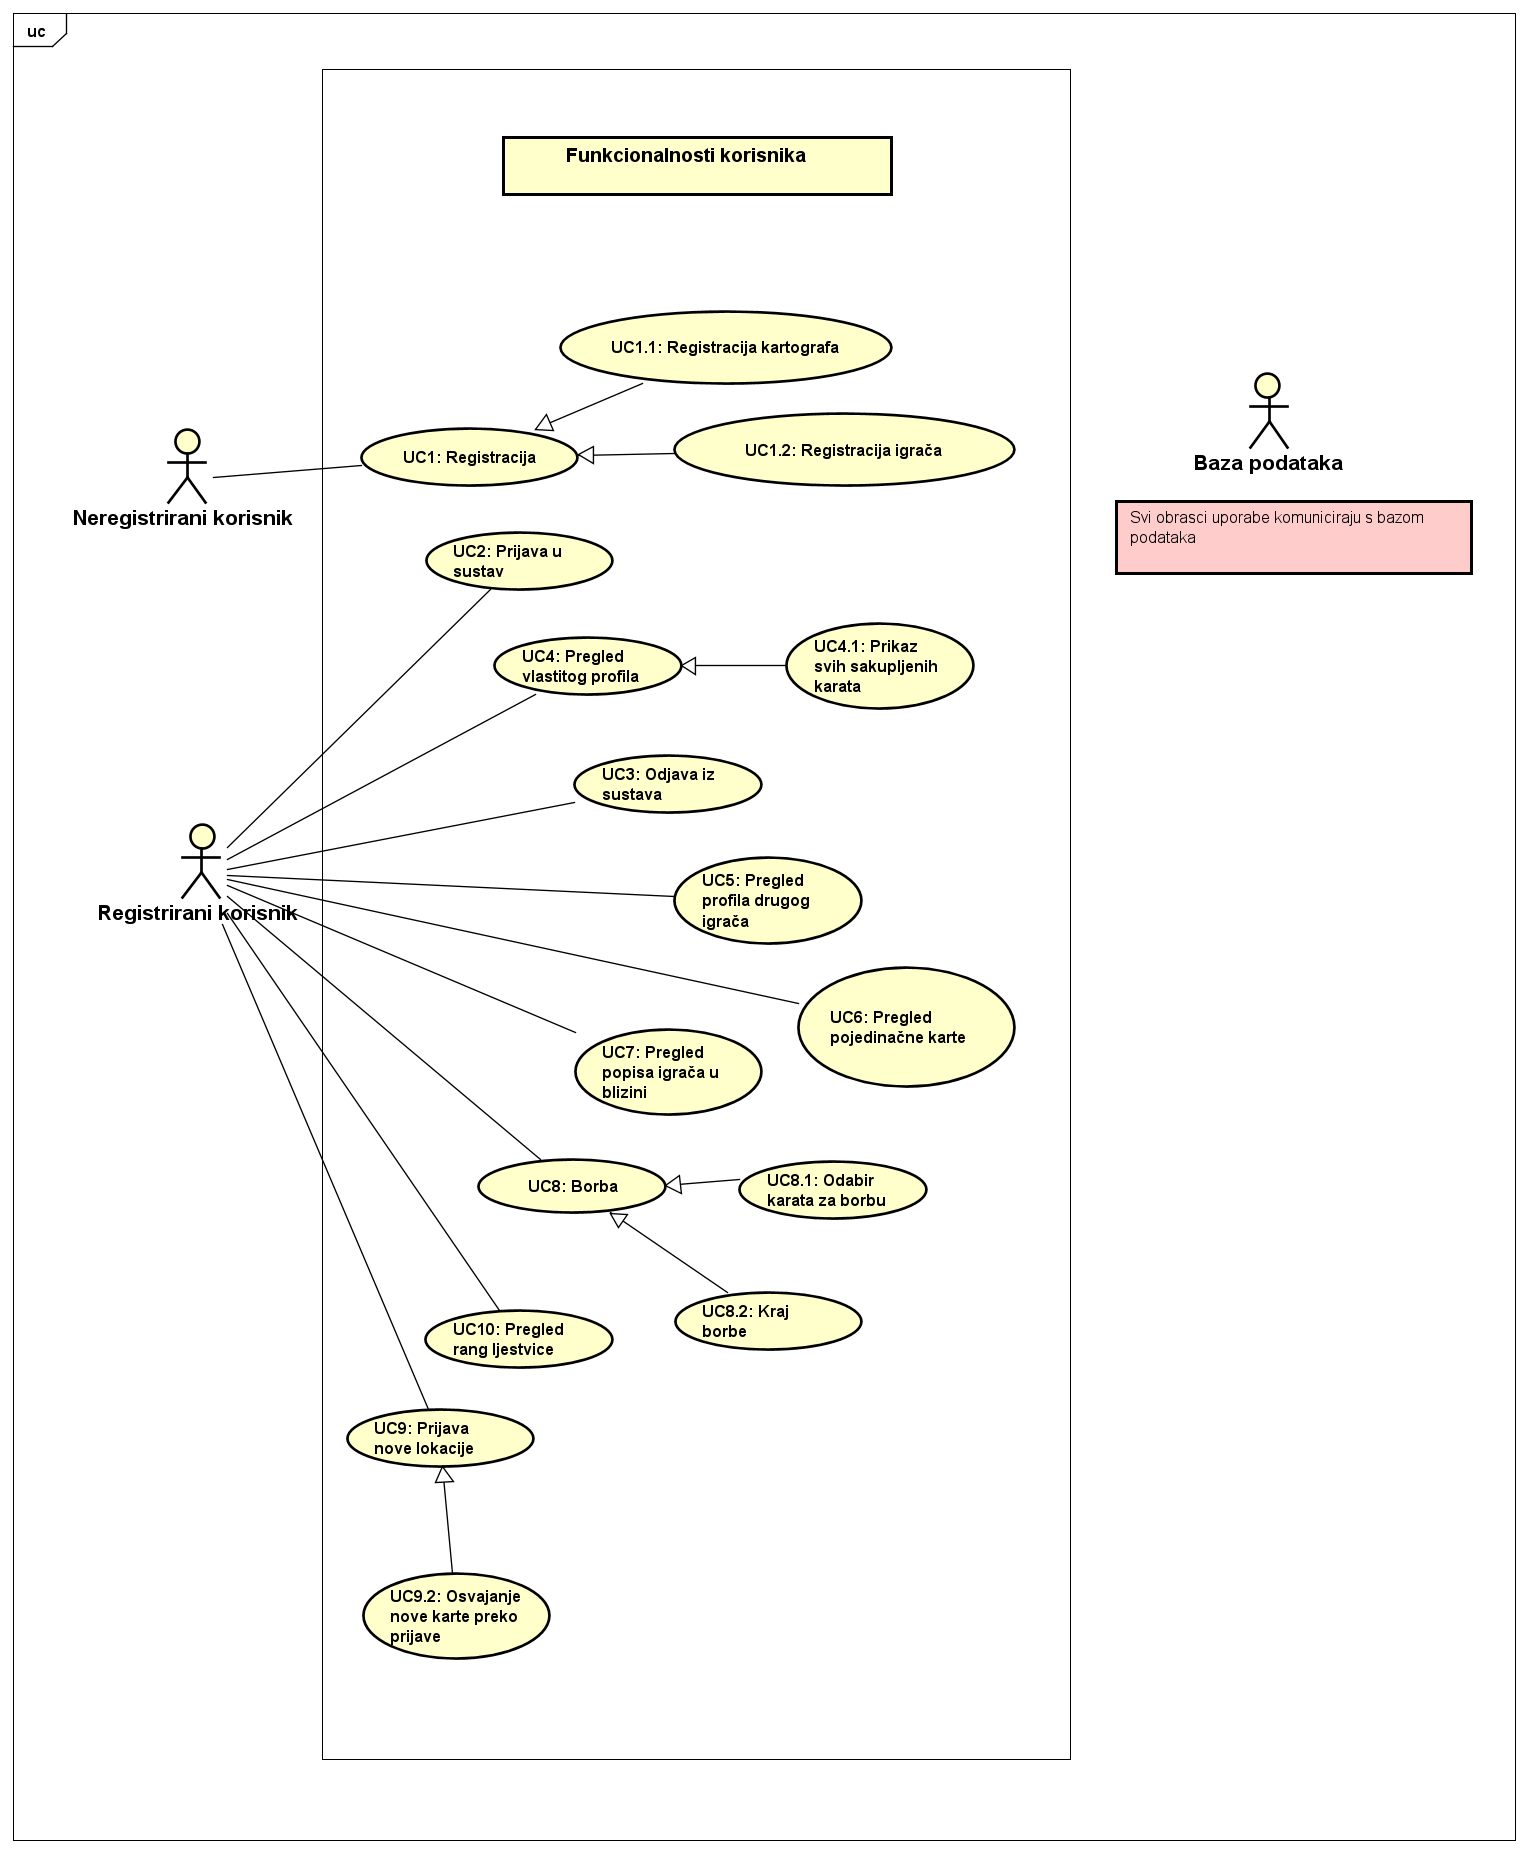
\includegraphics[scale=0.42]{dijagrami/funkcionalnosti_korisnika} \\
					\caption{Dijagram obrasca uporabe, funkcionalnosti neregistriranog i registriranog korisnika}
					\label{fig:funkcionalnosti_korisnika}
				\end{figure}
			
			\begin{figure}[H]
				\centering
				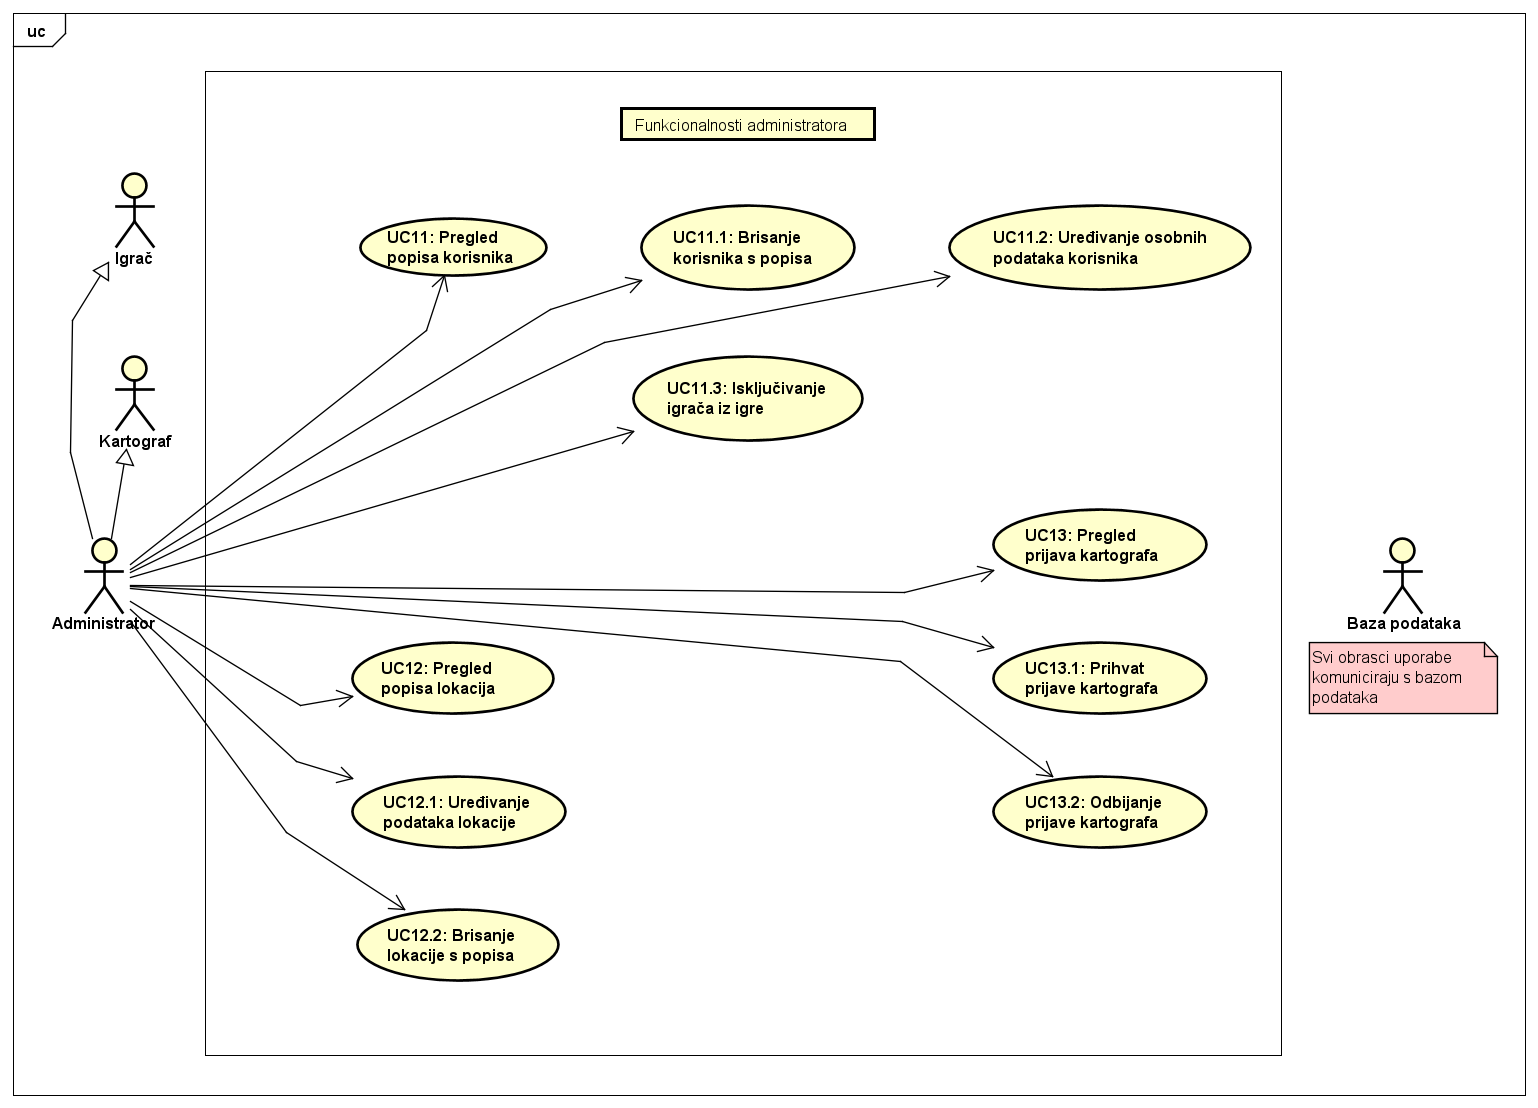
\includegraphics[scale=0.42]{dijagrami/funkcionalnosti_administratora} \\
				\caption{Dijagram obrasca uporabe, funkcionalnosti administratora}
				\label{fig:funkcionalnosti_administratora} 
			\end{figure}
		
		\begin{figure}[H]
			\centering
			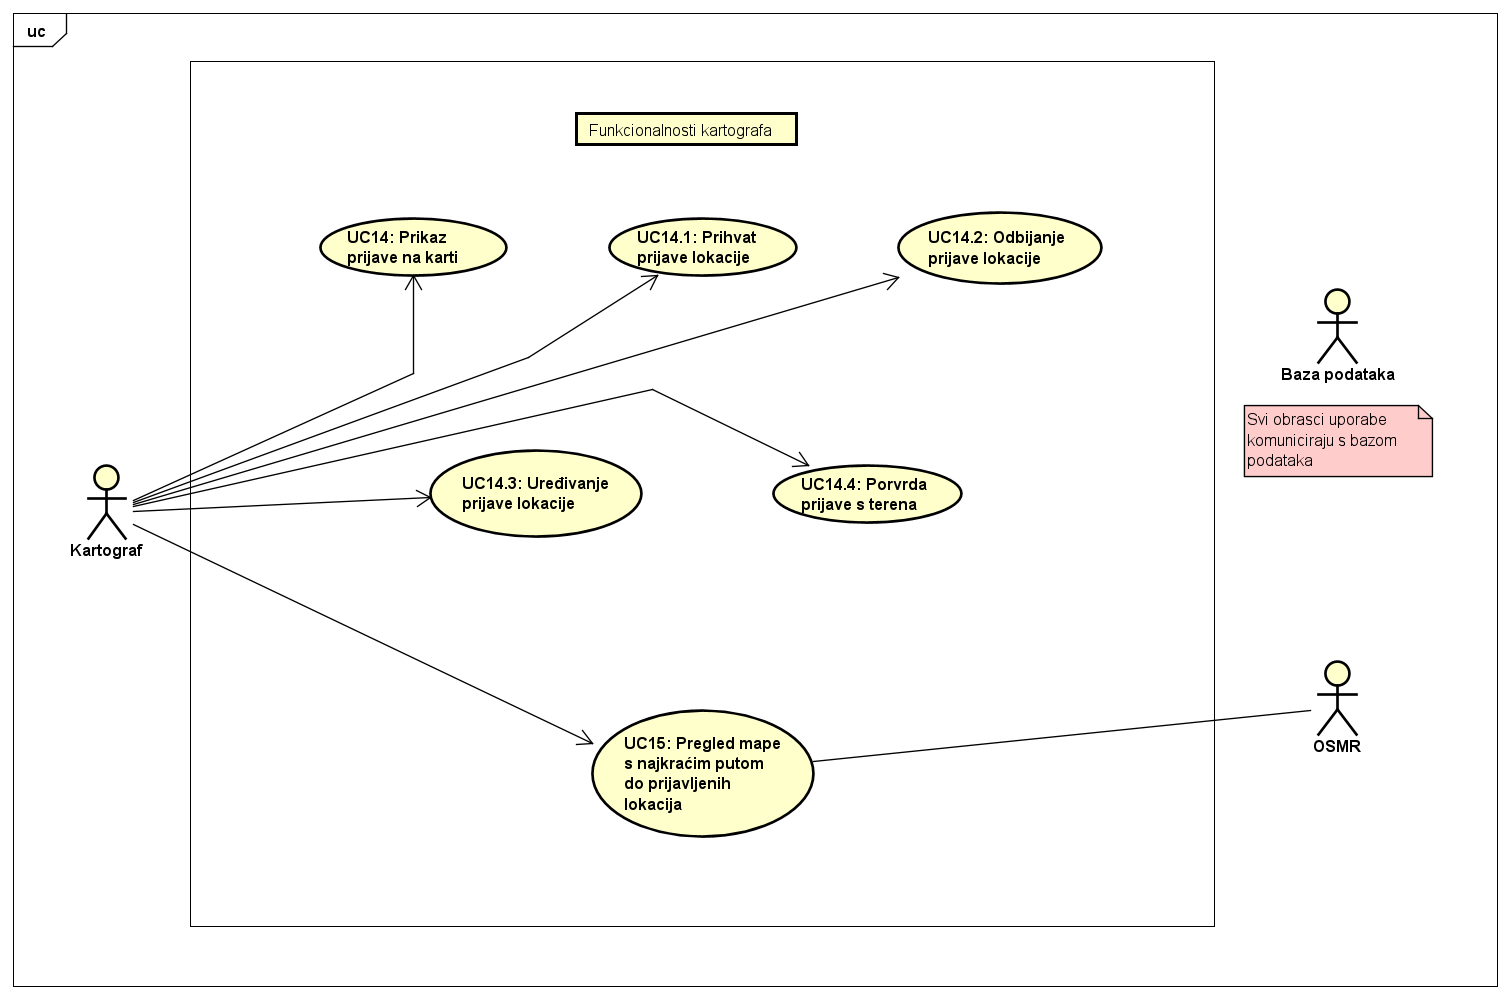
\includegraphics[scale=0.42]{dijagrami/funkcionalnosti_kartografa} \\
			\caption{Dijagram obrasca uporabe, funkcionalnosti kartografa}
			\label{fig:funkcionalnosti_kartografa} 
		\end{figure}
			\subsection{Sekvencijski dijagrami}
				
				\textbf{\textit{dio 1. revizije}}\\
				
				\textit{Nacrtati sekvencijske dijagrame koji modeliraju najvažnije dijelove sustava (max. 4 dijagrama). Ukoliko postoji nedoumica oko odabira, razjasniti s asistentom. Uz svaki dijagram napisati detaljni opis dijagrama.}
				\eject
				
				\begin{figure}[H]
					\centering
					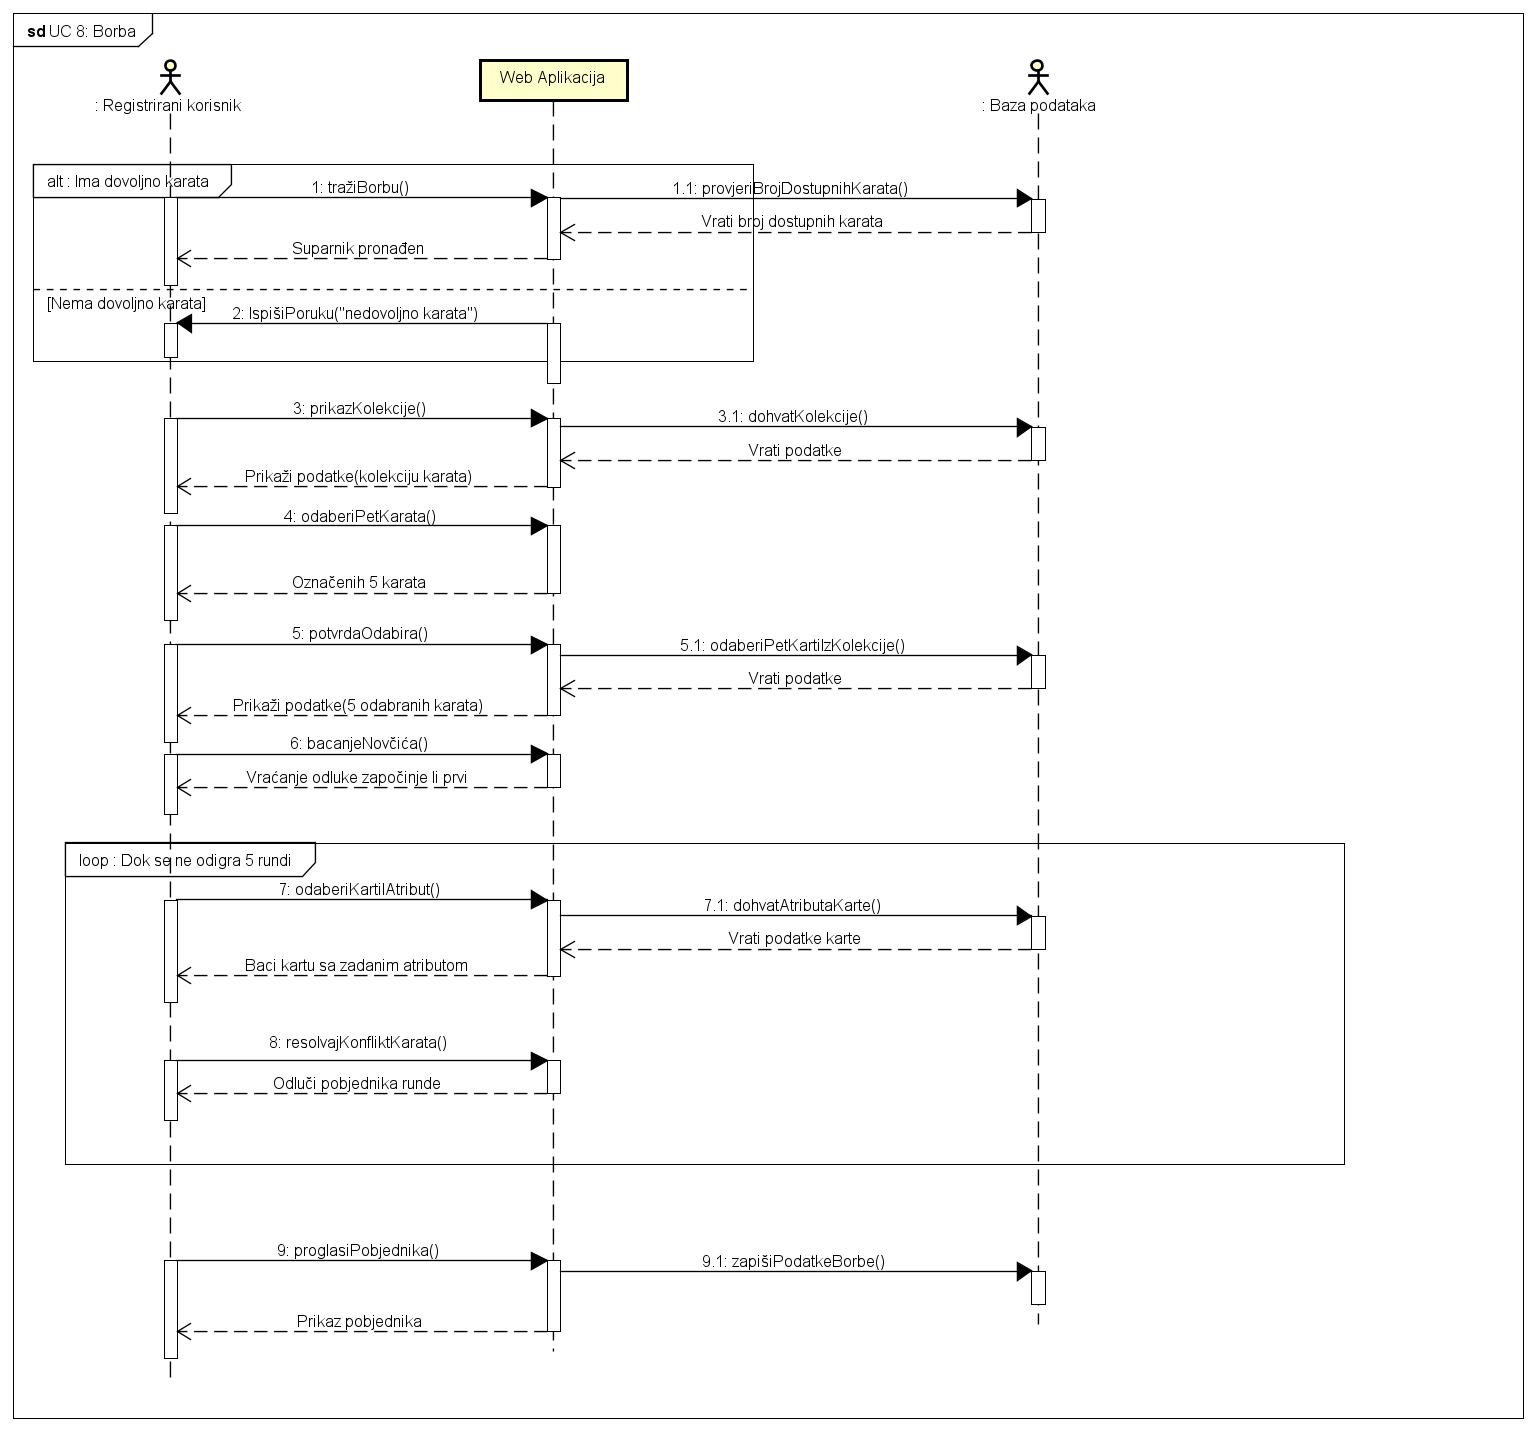
\includegraphics[scale=0.42]{dijagrami/UC 8_ Borba} \\
					\caption{Sekvencijski dijagram za UC8}
					\label{fig:funkcionalnosti_korisnika}
				\end{figure}
			\begin{figure}[H]
				\centering
				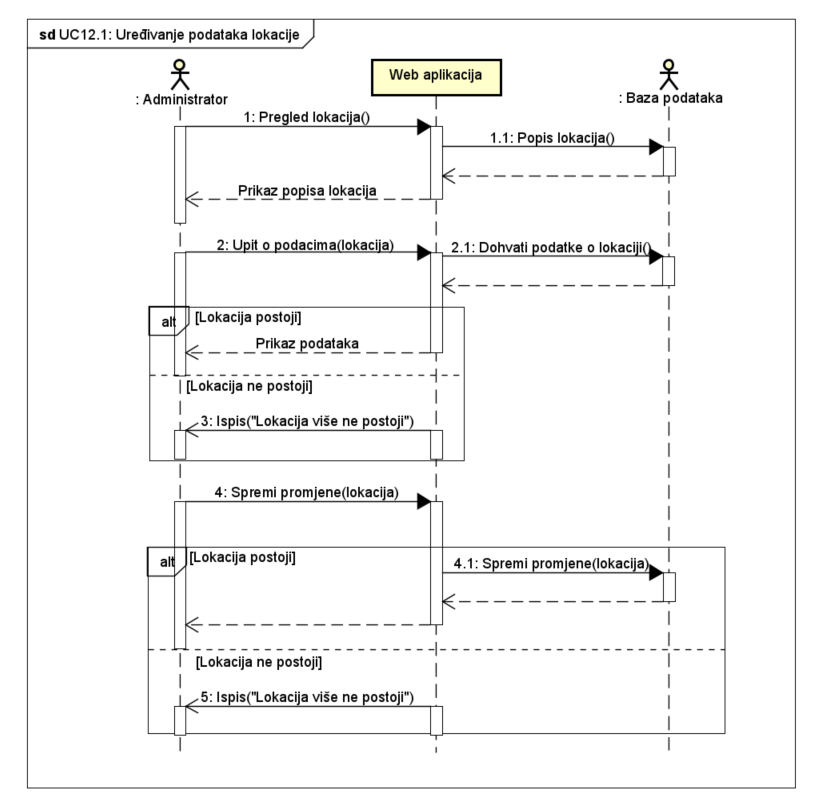
\includegraphics[scale=0.6]{dijagrami/UC12.1} \\
				\caption{Sekvencijski dijagram za UC12.1}
				\label{fig:funkcionalnosti_korisnika}
			\end{figure}
		\eject
	
		\section{Ostali zahtjevi}
		
			\textbf{\textit{dio 1. revizije}}\\
		 
			 \textit{Nefunkcionalni zahtjevi i zahtjevi domene primjene dopunjuju funkcionalne zahtjeve. Oni opisuju \textbf{kako se sustav treba ponašati} i koja \textbf{ograničenja} treba poštivati (performanse, korisničko iskustvo, pouzdanost, standardi kvalitete, sigurnost...). Primjeri takvih zahtjeva u Vašem projektu mogu biti: podržani jezici korisničkog sučelja, vrijeme odziva, najveći mogući podržani broj korisnika, podržane web/mobilne platforme, razina zaštite (protokoli komunikacije, kriptiranje...)... Svaki takav zahtjev potrebno je navesti u jednoj ili dvije rečenice.}
			 
			 
			 
	
	\chapter{Arhitektura i dizajn sustava}
		

	\textnormal{Pri procesu izbora arhitekture naše web aplikacije fokusirali smo se na klijent-server strukturu uz mogućnost odvojenih podsustava. U takvoj strukturi web poslužitelj osnova je rada web aplikacije. Njegova primarna zadaća je komunikacija klijenta s aplikacijom putem HTTP (\textit{engl. Hyper Text Transfer Protocol}) protokola. Korisnik šalje zahtjeve poslužitelju putem web preglednika. Web preglednik je program koji korisniku omogućuje pregled web-stranica i multimedijalnih sadržaja vezanih uz njih tako što stranicu pisanu u kodu interpretira na način da je razumljiva korisniku. Na temelju poslanih zahtjeva web aplikacija pristupa bazi podataka te vraća odgovor putem poslužitelja u obliku HTML dokumenta koji je vidljiv u pregledniku.}

	\begin{figure}[H]
		\centering
		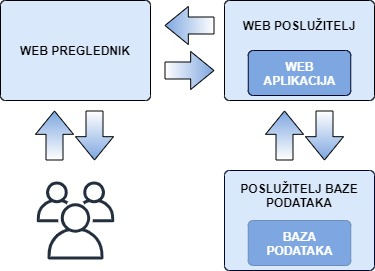
\includegraphics[scale=0.7]{slike/Arhitektura} \\
		\caption{ Organizacija sustava}
		\label{fig:arhitektura}
	\end{figure}

	\textnormal{Na temelju navedenih glavnih značajki i nadalje razrađenih obilježja odlučili smo se arhitekturu sustava bazirati na arhitekturnom stilu model-pogled-upravitelj (\textit{engl. Model-View-Controller, MVC}). Kod MVC stila, korisničko sučelje je odvojeno od ostatka sustava što nam omogućuje raspodjelu u odvojene timove tijekom rada na projektu. Mnogi programski okviri su izrađeni s MVC arhitekturom na umu, što omogućuje brži i jednostavniji razvoj aplikacije. Razinska kohezija elemenata postiže se kroz tri sloja, jednog na strani klijenta koji se naziva pogled (\textit{engl. view}) i dva na poslužiteljskoj strani, koji se nazivaju upravitelj (\textit{engl. controller}) i model (\textit{engl. model}), što nam uz povećanu koheziju i smanjivanje međuovisnosti omogućuje i fleksibilnost. Također smo izabrali ovaj arhitekturni stil zbog njegove mogućnosti jednostavne ponovne uporabe i nadogradnje pojedinačnih dijelova sustava, pošto se dodavanjem novih modela ili pogleda može brzo i jednostavno promijeniti aplikaciju. Time se pozitivno utječe i na planiranje zastare aplikacije, uz korištenje dobro poznatih tehnologija i jezika koji će biti detaljnije razrađeni u nastavku. Podjelom na navedene podsustave pojednostavili smo i testiranje tijekom izrade aplikacije jer se razni dijelovi sustava mogu neovisno testirati. Izborom web aplikacije pobrinuli smo se i za prenosivost, pošto se aplikaciji može pristupiti s velikog broja uređaja putem različitih web preglednika.}\\
	
	\textnormal{Negativna karakteristika MVC arhitekture može biti njezina glomaznost u pogledu velike količine datoteka što može usporiti sustav, no to ne smatramo problemom za ovaj projekt pošto je manjeg opsega.}\\
	
	\begin{figure}[H]
		\centering
		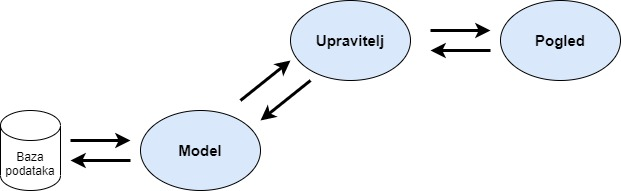
\includegraphics[scale=0.5]{slike/MVC} \\
		\caption{ MVC Arhitektura}
		\label{fig:arhitekturaMCV}
	\end{figure}

	\textnormal{U skladu s odabranom arhitekturom, aplikacija će biti razvijena u tri velike nezavisne komponente: pogled kroz \textit{front-end} sustav, te upravitelj i model kroz \textit{back-end} sustav i bazu podataka.}\\
	
	\textnormal{\textit{Front-end} predstavlja korisničko sučelje s kojim korisnik ima direktnu interakciju. Implementiran je pomoću programskog okvira Angular koristeći TypeScript, JavaScript, HTML i CSS. Za Angular smo se odlučili jer omogućava dizajniranje fleksibilnih komponenti visoke razine ponovne upotrebljivosti uz veliku responzivnost i interaktivnost. Uloge Angular servisa u ovoj aplikaciji su dostaviti sve potrebne podatke i skripte web poslužitelju korisnika, komunikacija s back end servisom i izvođenje vlastitih procesa koji su nužni za pravilan rad korisničkog sučelja. Razdvajanjem \textit{front-end} i \textit{back-end} servisa omogućavamo fokus na razvoj odličnog korisničkog sučelja što je bitan faktor korisnicima pri odabiru naše igre kao jedne od mnogo dostupnih.}\\
	
	\textnormal{\textit{Back-end} predstavlja servis koji upravlja \textit{front-end} servisom i dostavlja podatke korisniku te je zato centralna točka GeoFighter aplikacije. Implementiran je pomoću programskog okvira SpringBoot koristeći programski jezik Java. Omogućava pristup bazi podataka, komunikaciju HTTP zahtjevima te sadržava logiku i funkcionalnosti GeoFighter igre. Struktura \textit{back-end} servisa se fokusira na smanjivanje međuovisnosti sadržaja i izbjegava opću međuovisnost. Razdvajanjem \textit{front-end} i \textit{back-end} servisa smanjujemo opterećenost \textit{back-end} servisa}\\
	
	\textnormal{Baza podataka je trajno spremište svih podataka koje GeoFighter aplikacija treba sadržavati. Ona komunicira isključivo s \textit{back-end} servisom. Baza podataka je relacijskog tipa te je implementirana koristeći Postgres. Postgres baza podataka je odličan izbor za baze podataka male do srednje veličine te je vrlo fleksibilan izbor za zahtjeve koje ova aplikacija izvršava.}\\
	
	\begin{figure}[H]
		\centering
		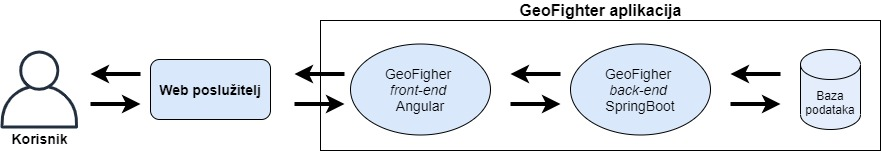
\includegraphics[scale=0.5]{slike/strukturaGF} \\
		\caption{Skica arhitekture sustava}
		\label{fig:arhitekturaGF}
	\end{figure}
	
	
				
		\section{Baza podataka}
			
			
		\textnormal{Za potrebe našeg sustava koristiti ćemo relacijsku bazu podataka koja svojom strukturom 	olakšava modeliranje stvarnog svijeta. Gradivna jedinka baze je relacija, odnosno tablica koja je definirana svojim imenom i skupom atributa, dok su odnosi između relacija definirani vezama. Zadaća baze podataka je brza i jednostavna pohrana, izmjena i dohvat podataka za daljnju obradu.\\Baza podataka ove aplikacije sastoji se od slijedećih tablica:}
		
		\begin{packed_item}
			\item \textnormal{Users}
			\item \textnormal{Tokens}
			\item \textnormal{Refresh\textunderscore token}
			\item \textnormal{Roles}
			\item \textnormal{Privileges}
			\item \textnormal{Roles\textunderscore privileges}
			\item \textnormal{Location\textunderscore cards}
			\item \textnormal{User\textunderscore card}
			\item \textnormal{Fights}
			\item \textnormal{User\textunderscore  card\textunderscore fight}
		\end{packed_item}
		
			\subsection{Opis tablica}
			

				\textnormal{\textbf{Users} \quad Ovaj entitet sadržava sve važne informacije o korisniku aplikacije koje bilježi atributima navedenim u tablici. U vezi je \textit{One-to-Many} s entitetima Tokens, Fights, Location\textunderscore cards i User\textunderscore card preko atributa user\textunderscore id. Također je u vezi \textit{Many-to-One} s entitetom Roles preko atributa role\textunderscore id.} \\
				
				\begin{longtabu} to \textwidth {|X[6, 3]|X[6, l]|X[20, l]|}
					
					\hline \multicolumn{3}{|c|}{\textbf{users}}	 \\[3pt] \hline
					\endfirsthead
					
					\hline \multicolumn{3}{|c|}{\textbf{users}}	 \\[3pt] \hline
					\endhead
					
					\hline 
					\endlastfoot
					
					\textbf{user\textunderscore id} & BIGSERIAL	&  	jedinstveni identifikator korisnika	\\ \hline
					email & VARCHAR & email adresa korisnika \\ \hline
					username & VARCHAR & korisničko ime \\ \hline
					password & VARCHAR & lozinka korisnika \\ \hline
					photourl & VARCHAR & poveznica na fotografiju profila \\ \hline
					created\textunderscore time & TIMESTAMP & trenutak stvaranja korisničkog računa  \\ \hline 
					current\textunderscore location & BYTEA	&  	trenutna lokacija korisnika	\\ \hline 
					elo\textunderscore score & INT4 & rang korisnika prema elo sustavu \\ \hline
					enabled & BOOLEAN & zastavica potvrde email adrese\\ \hline
					losses & INT4 & broj izgubljenih igara \\ \hline
					wins & INT4 & broj pobijeđenih igara \\ \hline
					online & BOOLEAN & zastavica prisutnosti korisnika \\ \hline
					forced\textunderscore timeout\textunderscore end & TIMESTAMP & trenutak mogućeg povratka u igru u slučaju privremenog isključenja \\ \hline
					cartographer\textunderscore status	& INT4 &   oznaka statusa pri prijavi za kartografa 	\\ \hline 
					iban & VARCHAR & IBAN bankovnog računa kartografa \\ \hline			
					id\textunderscore card\textunderscore photourl & VARCHAR & poveznica na fotografiju osobne iskaznice \\ \hline
					\textit{role\textunderscore id} & INT8 &  jedinstveni identifikator uloge (roles.role\textunderscore id)	\\ \hline 
					
					
				\end{longtabu}
			
				
				\textnormal{\textbf{Tokens} \quad Ovaj entitet sadržava sve važne informacije o tokenima koji se koriste za autentifikaciju korisnika. Atributi koje posjeduje su jedinstveni identifikator tokena, njegova vrijednost, datum isticanja te oznaku korisnika kojem pripada. U vezi je \textit{Many-to-One} s entitetom Users preko atributa "user\textunderscore user\textunderscore id".} \\
			
			
			
				\begin{longtabu} to \textwidth {|X[6, l]|X[6, l]|X[20, l]|}
					
					\hline \multicolumn{3}{|c|}{\textbf{tokens}}	 \\[3pt] \hline
					\endfirsthead
					
					\hline \multicolumn{3}{|c|}{\textbf{tokens}}	 \\[3pt] \hline
					\endhead
					
					\hline 
					\endlastfoot
					
					\textbf{id} & BIGSERIAL	&  	jedinstveni identifikator tokena 	\\ \hline
					expiry\textunderscore date	& TIMESTAMP &   datum isticanja tokena	\\ \hline 
					token & VARCHAR &  vrijednost tokena \\ \hline  
					\textit{"user\textunderscore user\textunderscore id"} & INT8 &  jedinstvena oznaka korisnika (users.user\textunderscore id) 	\\ \hline 
					
					
				\end{longtabu}
			
				\textnormal{}
			
				\textnormal{\textbf{Refresh\textunderscore token} \quad Ovaj entitet sadržava sve važne informacije o obnavljanju tokena koji služe za autentifikaciju korisnika. Atributi koje posjeduje su jedinstveni identifikator tokena, njegova nova vrijednost te datum stvaranja.} \\
				
			\begin{longtabu} to \textwidth {|X[6, l]|X[6, l]|X[20, l]|}
				
				\hline \multicolumn{3}{|c|}{\textbf{refresh\textunderscore token}}	 \\[3pt] \hline
				\endfirsthead
				
				\hline \multicolumn{3}{|c|}{\textbf{refresh\textunderscore token}}	 \\[3pt] \hline
				\endhead
				
				\hline 
				\endlastfoot
				
				\textbf{id} & BIGSERIAL &  	jedinstveni identifikator tokena (tokens.id) 	\\ \hline
				created\textunderscore date	& TIMESTAMP &   datum stvaranja tokena	\\ \hline 
				token & VARCHAR & vrijednost tokena  \\ \hline 
				
				
				
			\end{longtabu}
		
			\textnormal{}
		
			\textnormal{\textbf{Roles} \quad Ovaj entitet sadržava sve važne informacije vezane uz ulogu koju određeni korisnik može imati, a one su administrator, kartograf ili igrač. Atributi koje posjeduje su jedinstveni identifikator uloge i njezin naziv. U vezi je \textit{One-to-Many} s entitetom Users preko atributa role\textunderscore id. Također je u vezi \textit{Many-to-Many} s entitetom Privileges preko spojne tablice roles\textunderscore privileges.} \\
		
			\begin{longtabu} to \textwidth {|X[6, l]|X[6, l]|X[20, l]|}
				
				\hline \multicolumn{3}{|c|}{\textbf{roles}}	 \\[3pt] \hline
				\endfirsthead
				
				\hline \multicolumn{3}{|c|}{\textbf{roles}}	 \\[3pt] \hline
				\endhead
				
				\hline 
				\endlastfoot
				
				\textbf{role\textunderscore id} & INT8	&  	jedinstveni identifikator uloge 	\\ \hline
				name	& VARCHAR &   naziv uloge	\\ \hline 
							
				
			\end{longtabu}
		
			\eject
		
			\textnormal{\textbf{Privileges} \quad Ovaj entitet sadržava sve važne informacije o povlasticama koje uloge mogu imati. Atributi koje posjeduje su jedinstveni identifikator povlastice i njen naziv. U vezi je \textit{Many-to-Many} s entitetom Roles preko spojne tablice roles\textunderscore privileges.} \\
		
			\begin{longtabu} to \textwidth {|X[6, l]|X[6, l]|X[20, l]|}
				
				\hline \multicolumn{3}{|c|}{\textbf{privileges}}	 \\[3pt] \hline
				\endfirsthead
				
				\hline \multicolumn{3}{|c|}{\textbf{privileges}}	 \\[3pt] \hline
				\endhead
				
				\hline 
				\endlastfoot
				
				\textbf{privilege\textunderscore id} & INT8	&  	jedinstveni identifikator povlastice 	\\ \hline
				name	& VARCHAR &   naziv povlastice	\\ \hline 
								
				
			\end{longtabu}
		
			\textnormal{}
		
			\textnormal{\textbf{Roles\textunderscore privileges} \quad Ova tablica nastaje zbog \textit{Many-to-Many} veze između entiteta Roles i Privileges. Sadrži njihove primarne ključeve te je time povezana s njima. Prikazuje koje uloge imaju koje povlastice.} \\
			
			\begin{longtabu} to \textwidth {|X[6, l]|X[6, l]|X[20, l]|}
				
				\hline \multicolumn{3}{|c|}{\textbf{roles\textunderscore privileges}}	 \\[3pt] \hline
				\endfirsthead
				
				\hline \multicolumn{3}{|c|}{\textbf{roles\textunderscore privileges}}	 \\[3pt] \hline
				\endhead
				
				\hline 
				\endlastfoot
				
				\textbf{\textit{role\textunderscore id}} & INT8 & jedinstveni identifikator uloge (roles.role\textunderscore id) \\ \hline
				\textbf{\textit{privilege\textunderscore id}} & INT8	&  	jedinstveni identifikator povlastice (privileges.privilege\textunderscore id) 	\\ \hline
				
						
				
			\end{longtabu}
		
			\textnormal{}
		
			\textnormal{\textbf{Location\textunderscore cards} \quad Ovaj entitet sadržava sve važne informacije o karticama lokacije. Atributi koje posjeduje su navedeni u tablici. Važno je istaknuti atribute uncommonness, difficulty i population. Oni će određivati jačinu kartice tijekom borbe. Njihovim izborom postignuta je ravnoteža pri dodjeljivanju jačine kartice jer će lokacije koje su teže dostupne obično imati manju naseljenost. U vezi je \textit{Many-to-Many-to-Many} s entitetima Fights i Users preko spojne tablice User\textunderscore card\textunderscore fight. Također je u vezi \textit{Many-to-One} s entitetom Users preko atributa accepted\textunderscore by\textunderscore user \textunderscore id i atributa created\textunderscore by\textunderscore user \textunderscore id.} \\
		
			\begin{longtabu} to \textwidth {|X[6, 4]|X[6, l]|X[20, l]|}
				
				\hline \multicolumn{3}{|c|}{\textbf{location\textunderscore cards}}	 \\[3pt] \hline
				\endfirsthead
				
				\hline \multicolumn{3}{|c|}{\textbf{location\textunderscore cards}}	 \\[3pt] \hline
				\endhead
				
				\hline 
				\endlastfoot
				
				\textbf{lcd\textunderscore id} & INT8	&  	jedinstveni identifikator kartice lokacije 	\\ \hline
				name	& VARCHAR &   naziv lokacije	\\ \hline 
				accepted & BOOLEAN & zastavica koja označava je li lokacija odobrena \\ \hline
				created\textunderscore at & TIMESTAMP & trenutak stvaranja kartice lokacije \\ \hline
				description & TEXT & opis lokacije \\ \hline
				enabled\textunderscore date & TIMESTAMP & trenutak odobravanja kartice lokacije \\ \hline
				location & BYTEA & stvarna lokacija koju označava kartica lokacije \\ \hline
				check\textunderscore needed & BOOLEAN & zastavica koja označava potrebu za dodatnom potvrdom kartice lokacije \\ \hline
				photo & VARCHAR & digitalni zapis fotografije lokacije \\ \hline
				uncommonness & INT & atribut koji označava rijetkost kartice \\ \hline
				difficulty & INT & atribut koji označava težinu dostupnosti lokacije \\ \hline
				population & INT & atribut koji označava naseljenost lokacije \\ \hline
				\textit{accepted\textunderscore by\textunderscore user \textunderscore id} & INT8 & jedinstveni identifikator kartografa koji je odobrio karticu lokacije (users.user\textunderscore id) \\ \hline
				\textit{created\textunderscore by\textunderscore user \textunderscore id} & INT8 & jedinstveni identifikator igrača koji je prijavio karticu lokacije (users.user\textunderscore id) \\ \hline				
				
				
			\end{longtabu}
		
			\textnormal{}
		
			\textnormal{\textbf{User\textunderscore card} \quad Ovaj entitet sadržava sve informacije o kartici koju posjeduje neki igrač. Atributi koje posjeduje su jedinstveni identifikator korisnika i kartice koju posjeduje, trenutak kada se kartica može ponovo koristit u borbi te koeficijent koji utječe na smanjenje broja bodova kartice. U vezi je \textit{Many-to-One} s entitetom Users preko atributa user\textunderscore id te s entitetom Location\textunderscore cards preko atribut lcd\textunderscore id.} \\
		
			\begin{longtabu} to \textwidth {|X[6, 4]|X[6, l]|X[20, l]|}
				
				\hline \multicolumn{3}{|c|}{\textbf{user\textunderscore card}}	 \\[3pt] \hline
				\endfirsthead
				
				\hline \multicolumn{3}{|c|}{\textbf{user\textunderscore card}}	 \\[3pt] \hline
				\endhead
				
				\hline 
				\endlastfoot
				
				\textbf{user\textunderscore id} & INT8	&  	jedinstveni identifikator korisnika koji posjeduje karticu lokacije (users.user\textunderscore id) 	\\ \hline
				\textbf{lcd\textunderscore id} & INT8	&  	jedinstveni identifikator kartice lokacije koju korisnik posjeduje (location\textunderscore cards.lcd\textunderscore id) 	\\ \hline
				cooldown\textunderscore end	& TIMESTAMP &   trenutak kada se kartica lokacije može ponovo koristiti u borbi	\\ \hline 
				cooldown\textunderscore multiplier & FLOAT8 & koeficijent prema kojem kartica lokacije gubi bodove \\ \hline
				
				
			\end{longtabu}
		
			\textnormal{}
		
			\textnormal{\textbf{Fights\textunderscore cards} \quad Ovaj entitet sadržava sve važne informacije o borbama koje su se odvile. Atributi koje posjeduje su jedinstveni identifikator borbe, vrijeme početka borbe te igrača koji je pobijedio. navedeni u tablici. U vezi je \textit{Many-to-Many-to-Many} s entitetima Location\textunderscore cards i Users preko spojne tablice User\textunderscore card\textunderscore fight. Također je u vezi \textit{Many-to-One} s entitetom Users preko atributa winner\textunderscore user \textunderscore id.}
		
			\begin{longtabu} to \textwidth {|X[6, l]|X[6, l]|X[20, l]|}
				
				\hline \multicolumn{3}{|c|}{\textbf{fights}}	 \\[3pt] \hline
				\endfirsthead
				
				\hline \multicolumn{3}{|c|}{\textbf{fights}}	 \\[3pt] \hline
				\endhead
				
				\hline 
				\endlastfoot
				
				\textbf{fight\textunderscore id} & INT8	&  	jedinstveni identifikator borbe 	\\ \hline
				start\textunderscore time	& TIMESTAMP &   trenutak početka borbe	\\ \hline 
				\textit{winner\textunderscore user\textunderscore id} & INT8 & jedinstveni identifikator korisnika koji je pobijedio u borbi (users.user\textunderscore id) \\ \hline
				
				
			\end{longtabu}
		
			\textnormal{}
		
			\textnormal{\textbf{User\textunderscore card\textunderscore fight} \quad Ova tablica nastaje zbog \textit{Many-to-Many-to-Many} veze između entiteta Users, Fight i Location\textunderscore cards. Sadrži njihove primarne ključeve te je time i povezana s njima, a prikazuje borbu u kojoj je korisnik sudjelovao s određenom karticom.} \\
		
			\begin{longtabu} to \textwidth {|X[6, l]|X[6, l]|X[20, l]|}
				
				\hline \multicolumn{3}{|c|}{\textbf{user\textunderscore card\textunderscore fight}}	 \\[3pt] \hline
				\endfirsthead
				
				\hline \multicolumn{3}{|c|}{\textbf{user\textunderscore card\textunderscore fight}}	 \\[3pt] \hline
				\endhead
				
				\hline 
				\endlastfoot
				
				\textbf{\textit{fight\textunderscore id}} & INT8	&  	jedinstveni identifikator borbe (fights.fight\textunderscore id) 	\\ \hline
				
				\textbf{\textit{user\textunderscore id}} & INT8	&  	jedinstveni identifikator igrača (users.user\textunderscore id) 	\\ \hline
				
				\textbf{\textit{lcd\textunderscore id}} & INT8	&  	jedinstveni identifikator kartice lokacije (location\textunderscore cards.lcd\textunderscore id) 	\\ \hline
				
				
			\end{longtabu}
			\eject
			\subsection{Dijagram baze podataka}
								
				\begin{figure}[H]
					\centering
					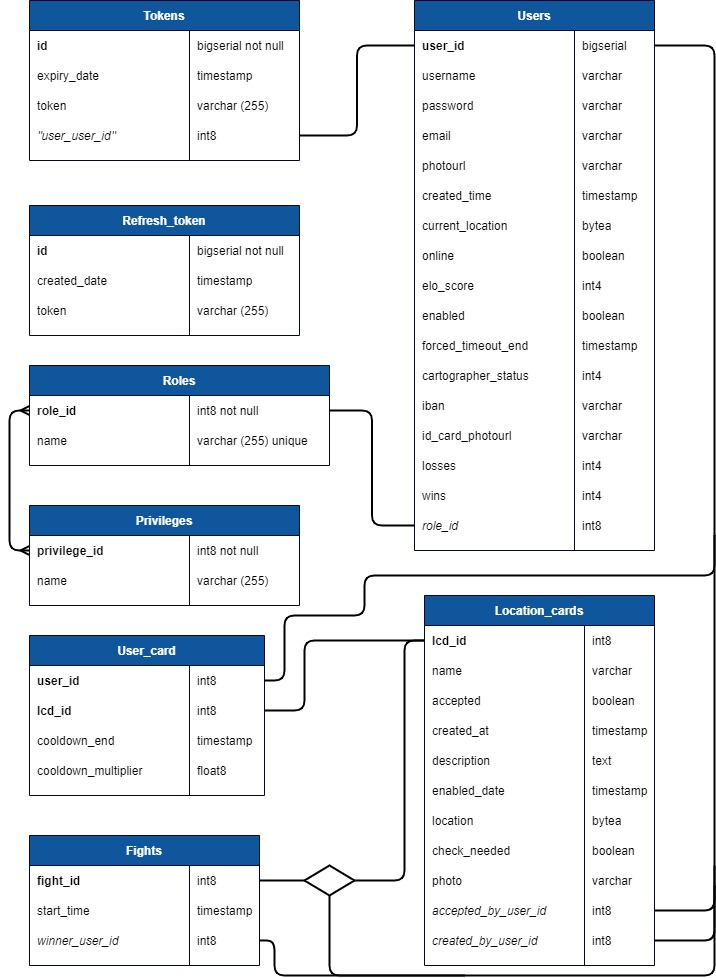
\includegraphics[scale=0.55]{slike/GeoFighterModel} 
					\caption{ER dijagram baze podataka}
					\label{fig:ERmodel}
				\end{figure}				
				
				
			
			\eject
			
			
		\section{Dijagram razreda}
		
			
			\textnormal{
				Na slijedećim slikama prikazani su razredi i sučelja koji pripadaju \textit{back-end} servisu izrađenom koristeći programski okvir SpringBoot i programski jezik Java. Svi razredi imaju implementirane get i set metode za vlastite atribute pomoću Lombok sustava iako se to eksplicitno ne navodi na dijagramima.
			} \\
			
			\textnormal{
				Na slici 4.5 prikazan je Controllers dio \textit{back-end} aplikacije. Upravljači (engl. controllers) su jedina izložena točka u aplikaciji te služe za komunikaciju s \textit{front-end} servisom koji nad njima izvršava upite. U svim upravljačima implementiran je Spring Security koji osigurava zaštićenost upravljača tako što u svakom zahtjevu koji pristigne na upravljač autorizira token koji se nalazi u zaglavlju zahtjeva. Ako zahtjev dobije pristup upravljaču, poziva se odgovarajući servisni sloj aplikacije koji izvršava svu logiku vezanu uz određenu značajku aplikacije. Upravljači zatim na \textit{front-end} vraćaju prikupljene informacije.
			}
			
			\begin{figure}[H]
				\centering
				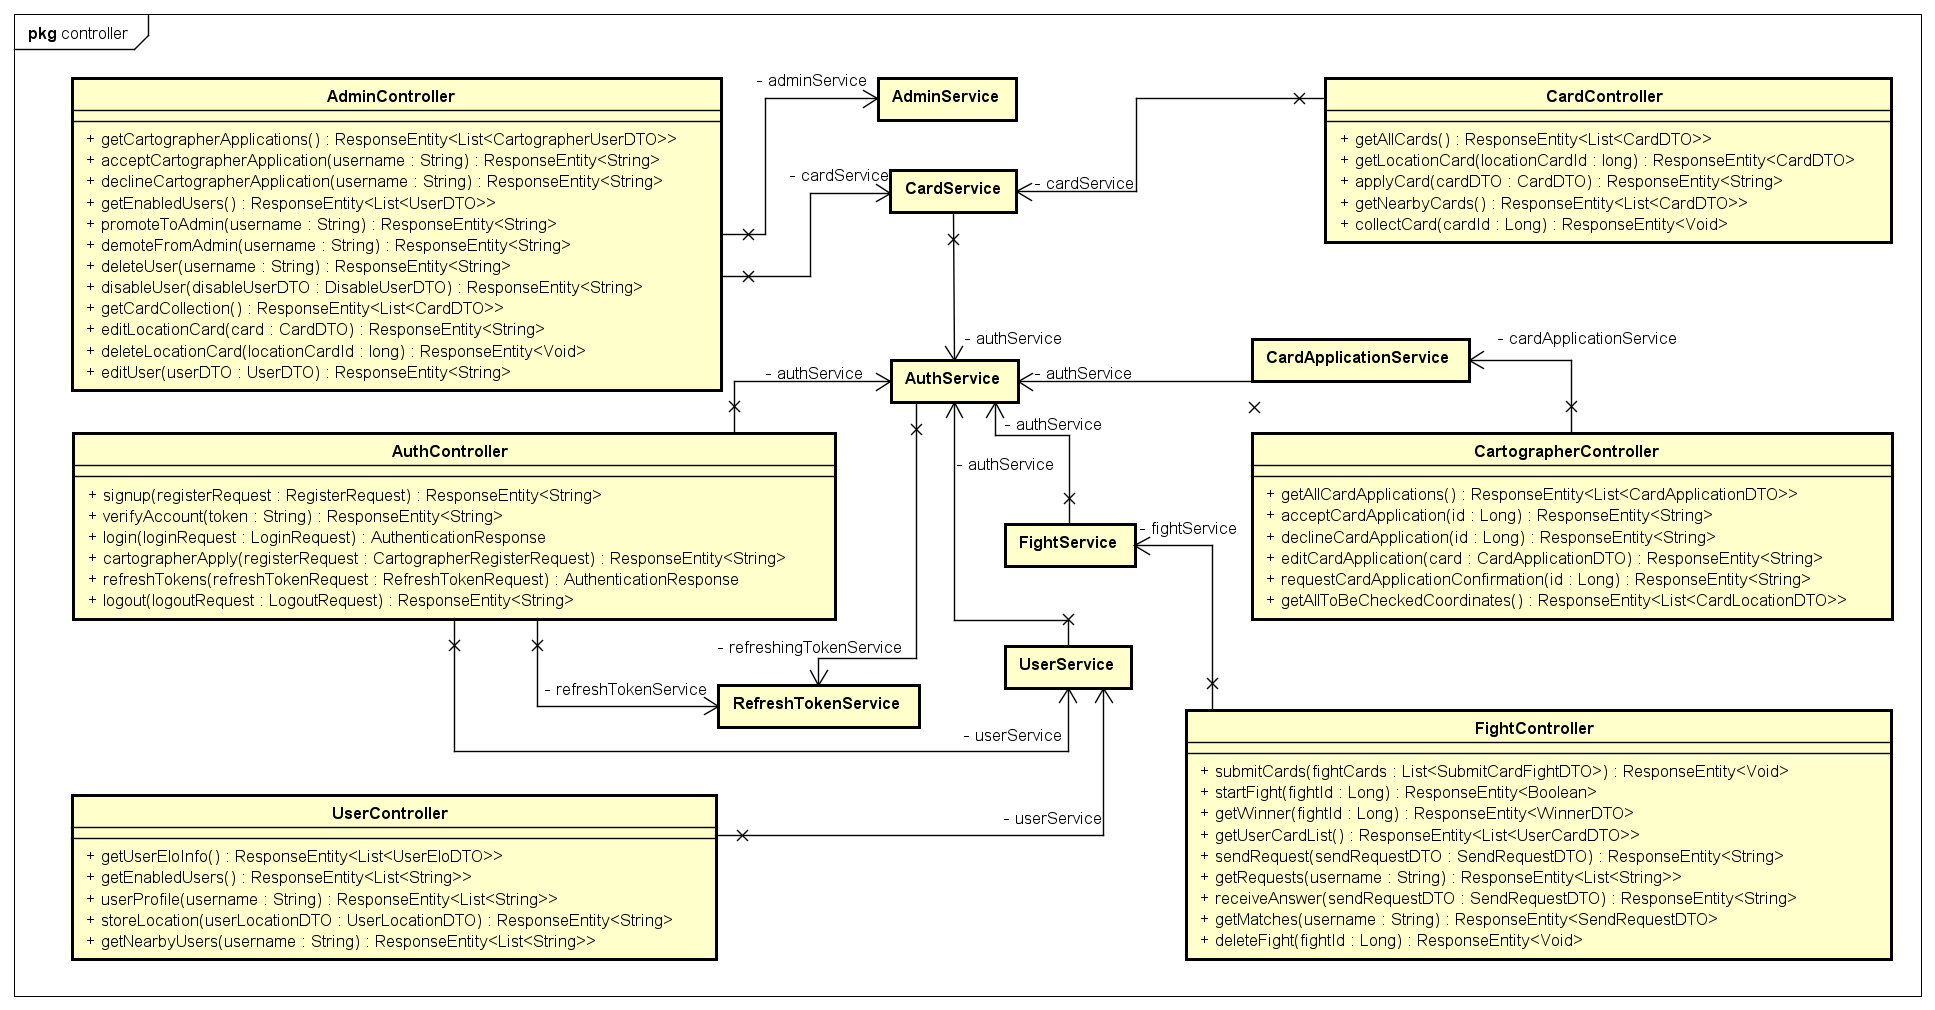
\includegraphics[scale=0.45]{dijagrami/Controller_CD} \\
				\caption{Dijagram razreda - Controllers}
				\label{fig:ControllerCD}
			\end{figure}
		
			\textnormal{
				DTO razredi prikazani su na slici 4.6. DTO (engl. data transfer object) služi za prijenos određenog dijela informacija iz \textit{back-end} sustava na \textit{front-end} i obrnuto. Sadrže primitivne tipove podataka u koje zatim spremamo odgovarajuće dijelove podataka iz baze, ili interpretiramo podatke pristigle s \textit{front-end} dijela aplikacije. 
			}
		
			\begin{figure}[H]
				\centering
				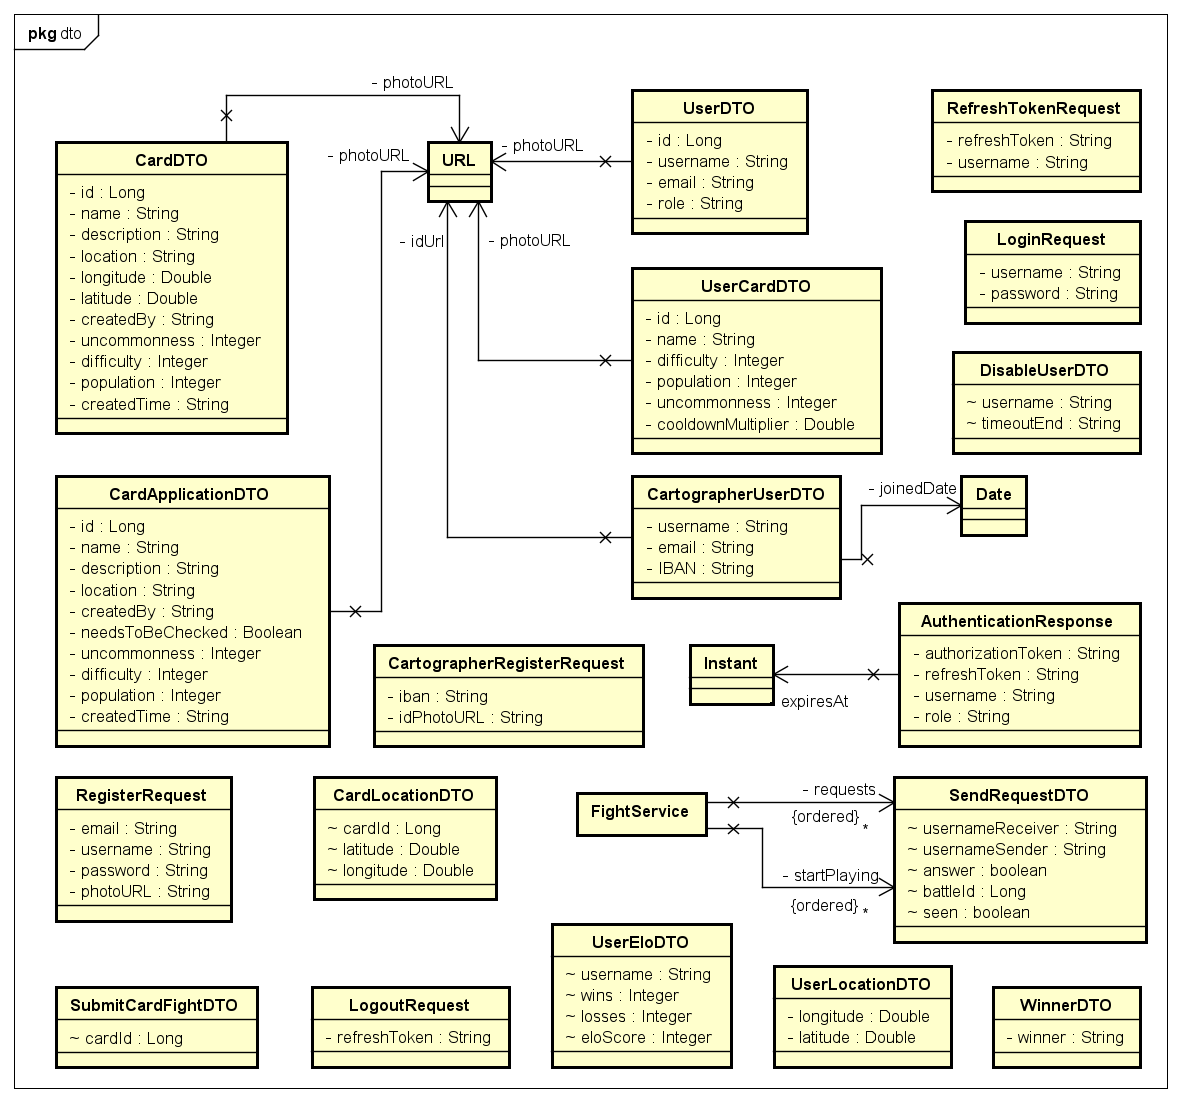
\includegraphics[scale=0.72]{dijagrami/DTO_CD} \\
				\caption{Dijagram razreda - DTO}
				\label{fig:DTO_CD}
			\end{figure}
		
			\textnormal{
				Na slici 4.7.prikazani su razredi servisnog sloja aplikacije. Servisi komuniciraju s
				repozitorijima koji pristupaju bazi i upravljačima od kojih dobivaju i kojima
				vraćaju podatke. Servisi iz baze dobivaju podatke te ih zatim obrađuju ovisno o poslovnoj logici i vraćaju rezultat.Servisi sadrže svu poslovnu logiku. Gotovo svaki upravljač ima pripadajući servis, a svaki je servis logički objedinjen skup funkcija poslovne logike.
			}
		
			\begin{figure}[H]
				\centering
				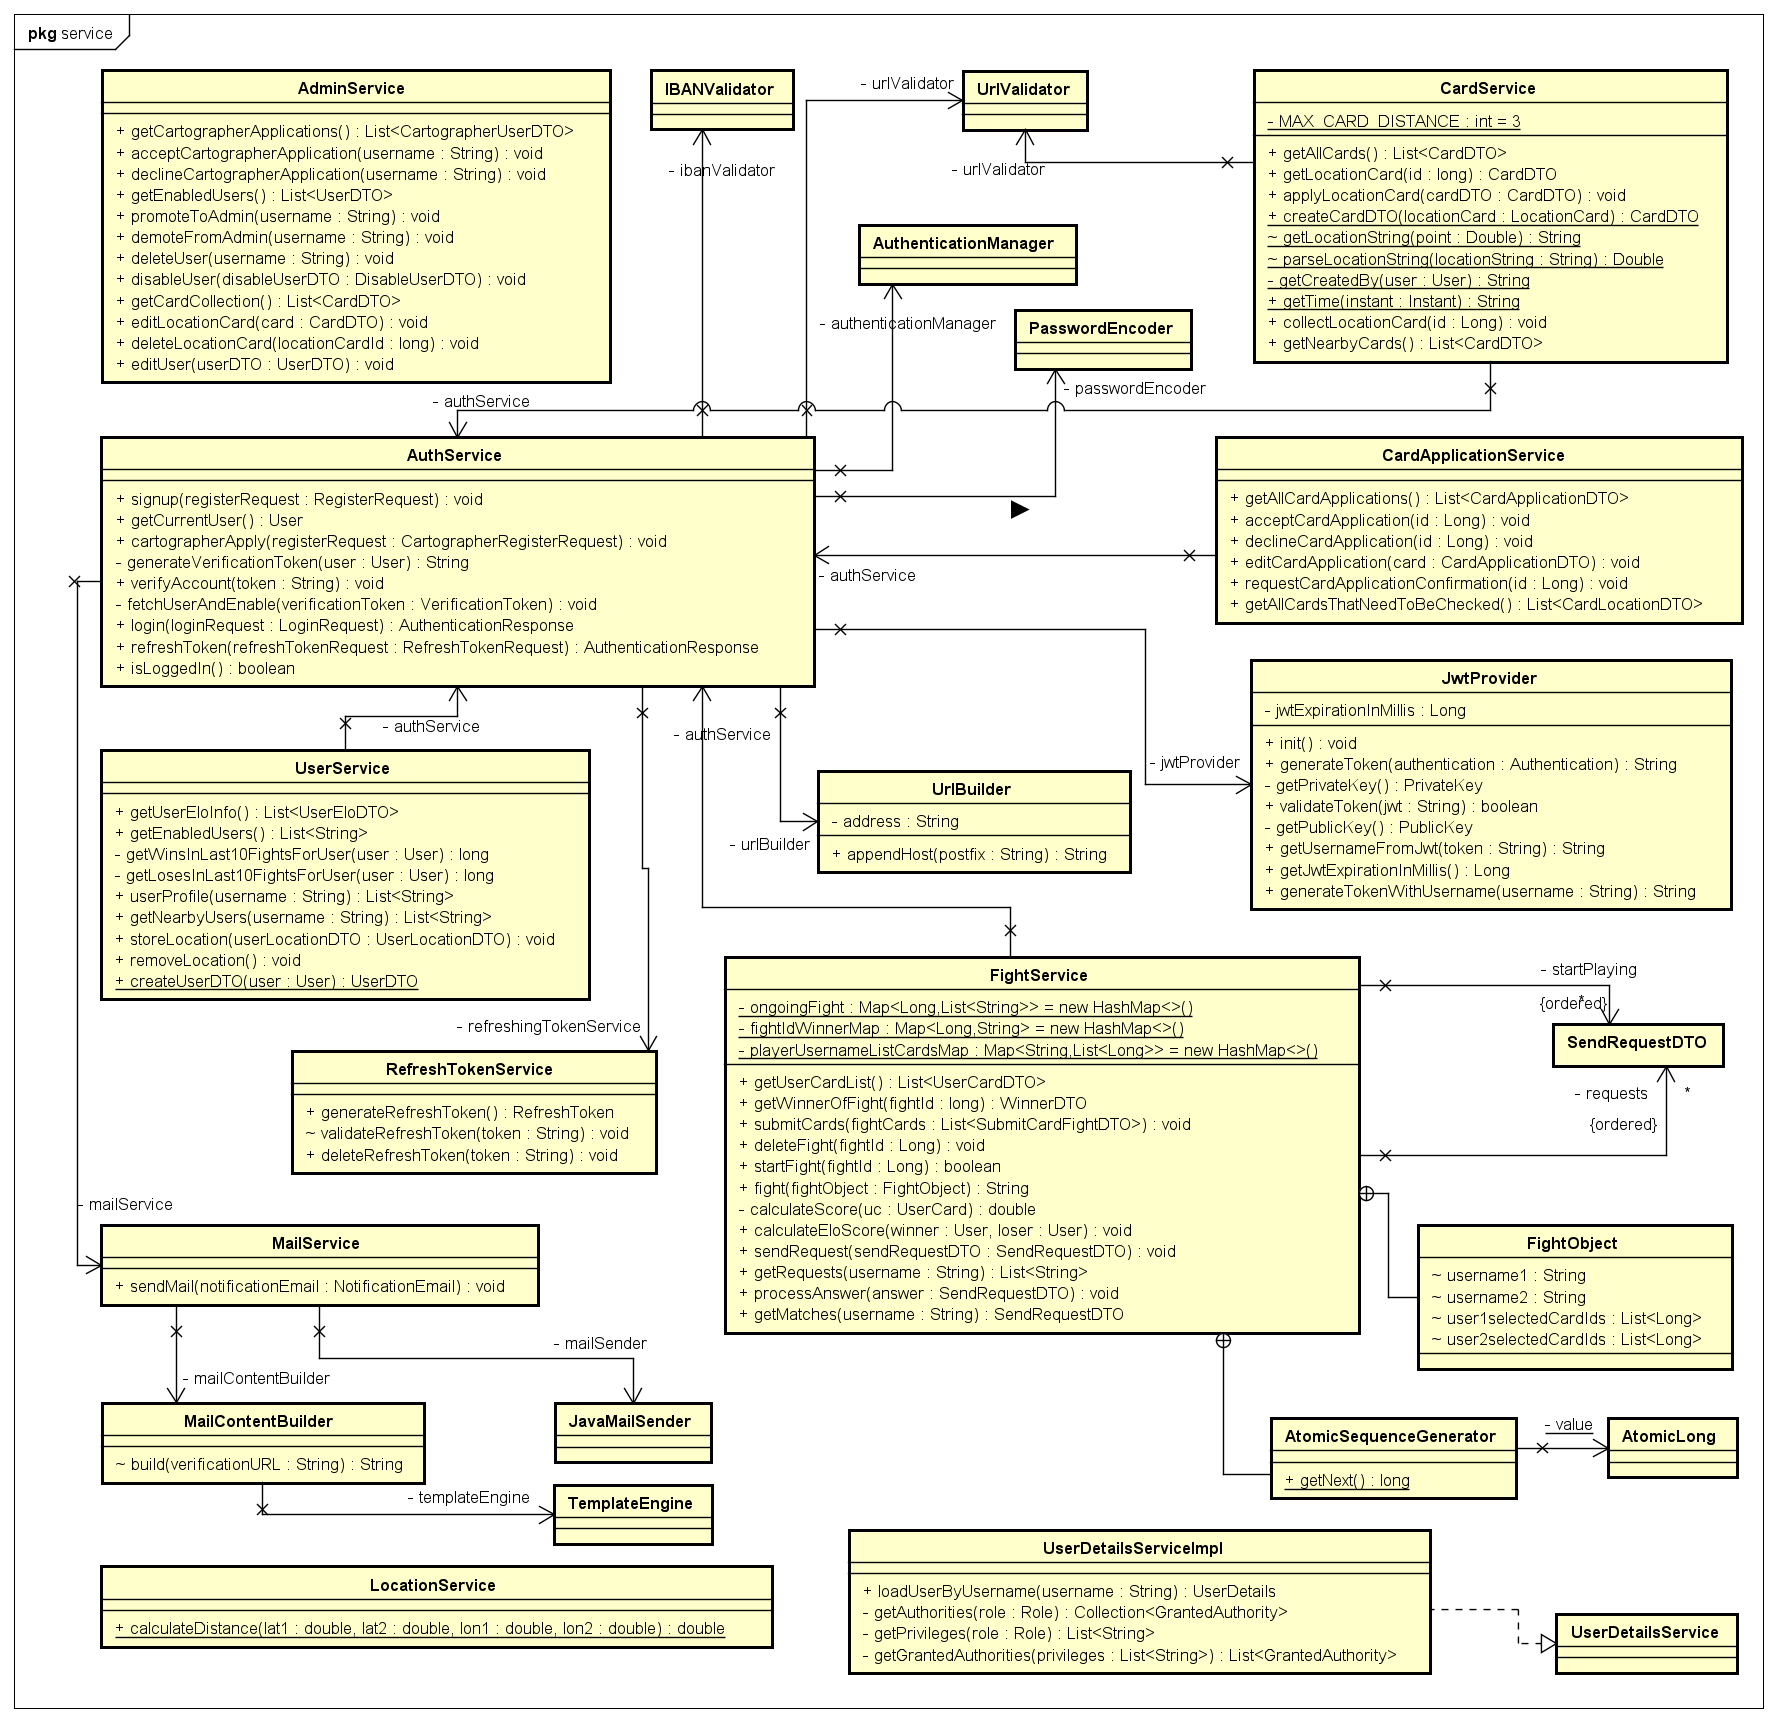
\includegraphics[scale=0.5]{dijagrami/Service_CD} \\
				\caption{Dijagram razreda - Service}
				\label{fig:Service_CD}
			\end{figure}
		
			\textnormal{
				Slika 4.8 prikazuje repozitorije. U ovoj aplikaciji za svaki entitet definiran
				je zasebni repozitorij koji nasljeđuje JpaRepository. Jpa Repository sadrži osnovne
				metode za dohvat podataka, a Spring Boot omogućuje programeru da specificiranjem
				samo imena metode može koristiti implementaciju iste.
			}
		
				\begin{figure}[H]
				\centering
				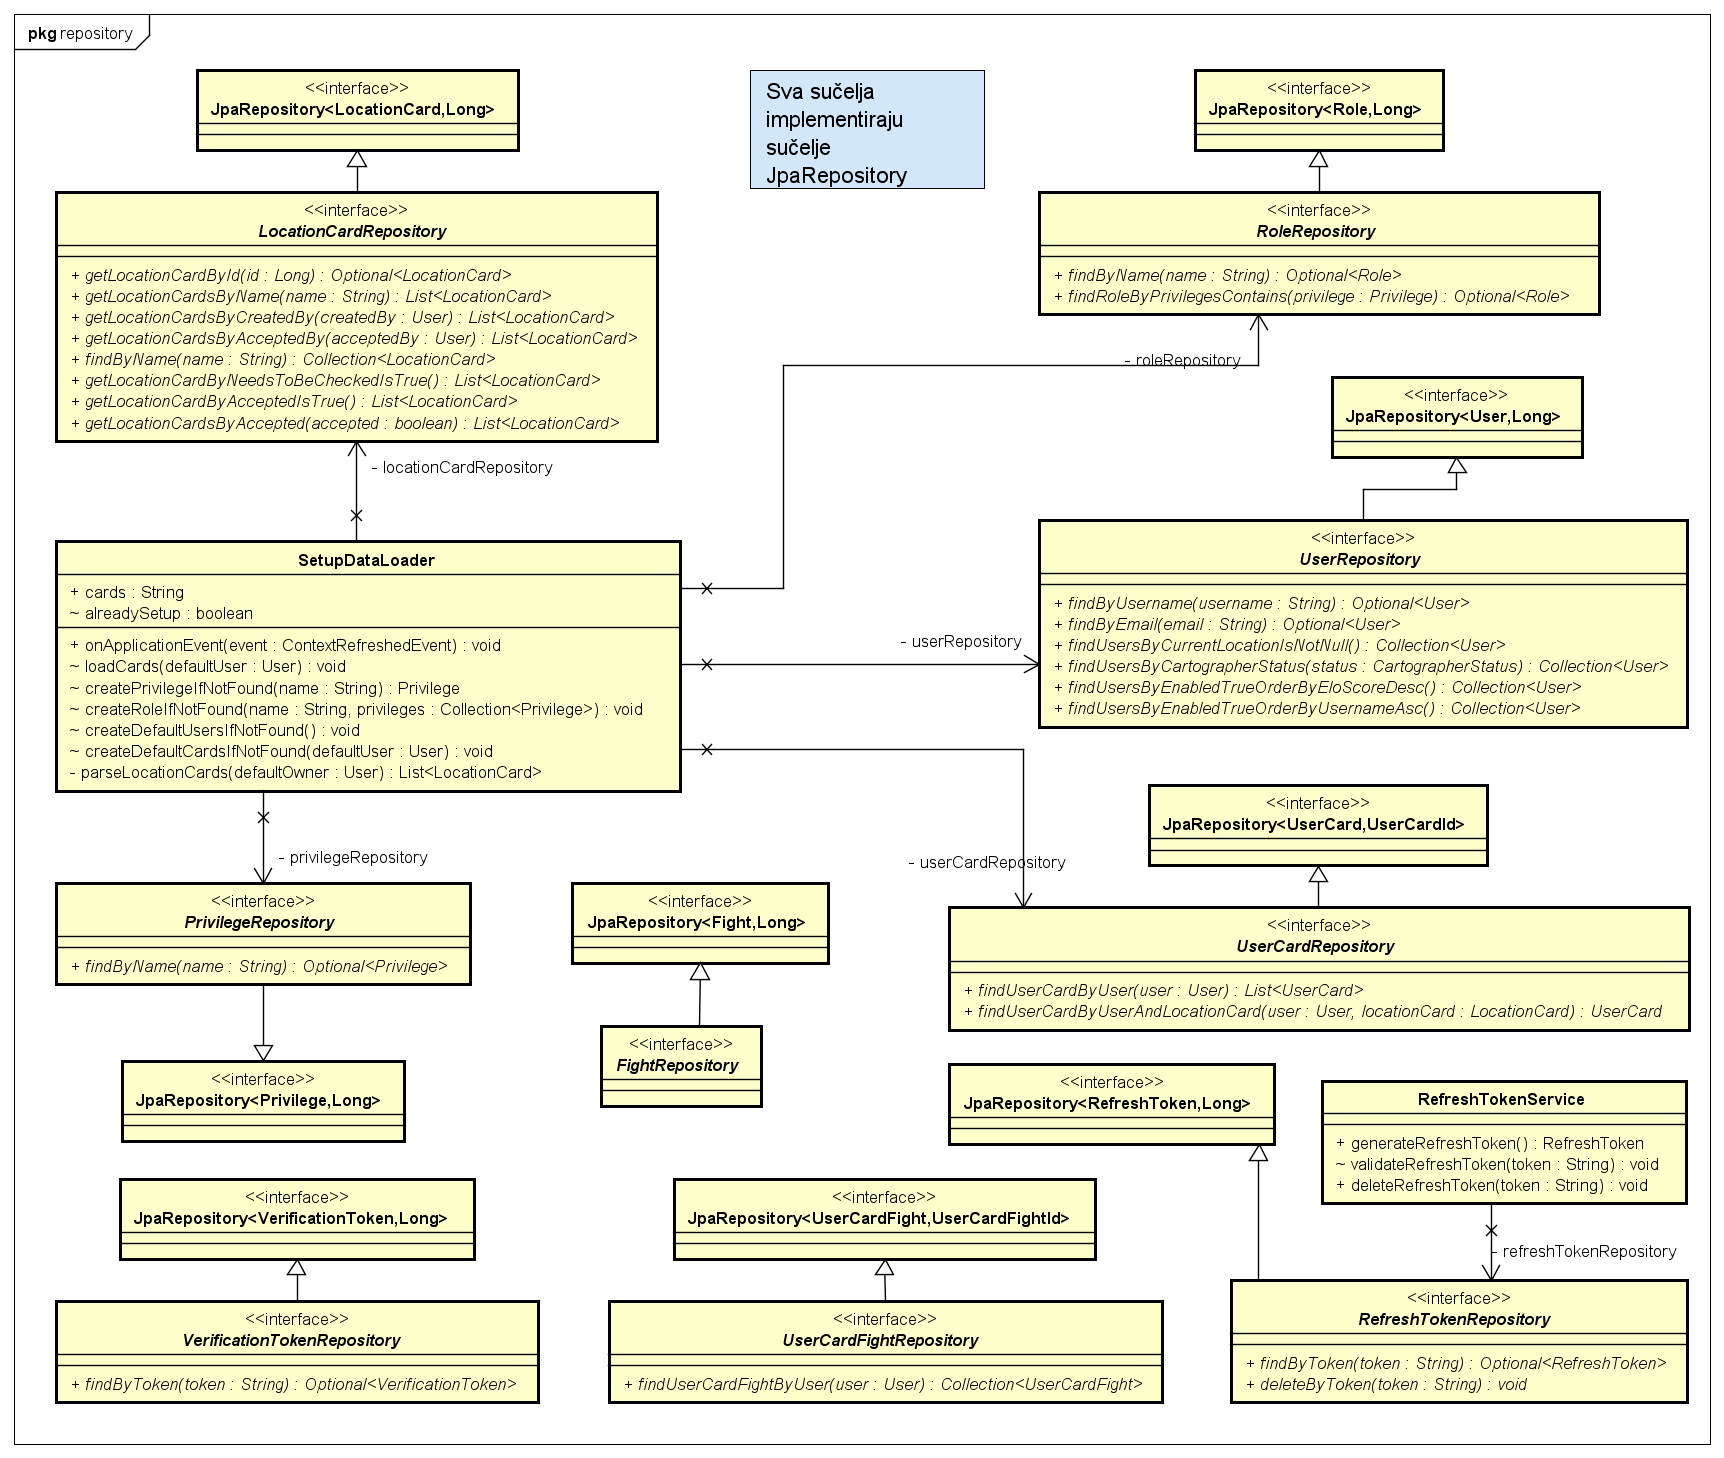
\includegraphics[scale=0.5]{dijagrami/Repository_CD} \\
				\caption{Dijagram razreda - Repository}
				\label{fig:Repository_CD}
			\end{figure}
							
			\textnormal{
				Model razredi prikazani na slici 4.9 preslikavaju strukturu baze podataka u aplikaciju. Razred User predstavlja korisnika koji se može registrirati u sustav koristeći osnovne informacije. Razred LocationCard predstavlja karticu lokacije, dok razred UserCard predstavlja posjedovanje same kartice od strane nekog korisnika.Razredi CartographerStatus, Role i Privilege služe kako bi se pobliže definirao svaki korisnik.
			}
			
			\begin{figure}[H]
				\centering
				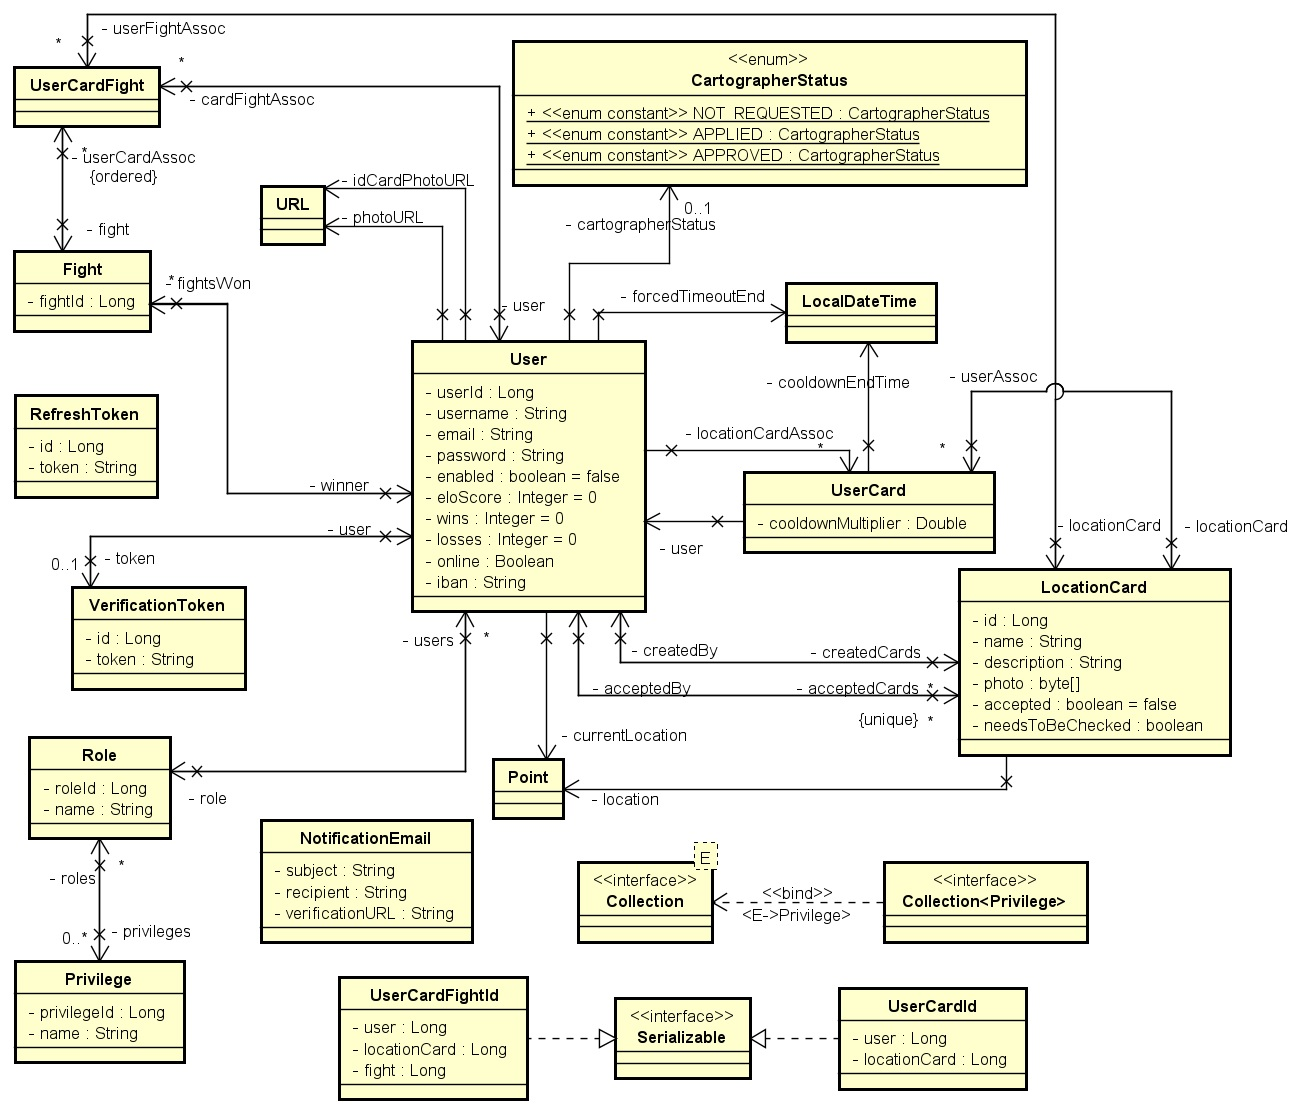
\includegraphics[scale=0.75]{slike/modelCD} \\
				\caption{Dijagram razreda - Model}
				\label{fig:modelCD}
			\end{figure}
		
			\textnormal{
				Na slici 4.10. prikazan je dijagram razreda vezanih uz Spring Security. Ulazna
				točka za autorizaciju zahtjeva je definirana u razredu JwtAuthenticationFilter koji poziva UserDetailsServiceImpl te zatim provjerava postoji li u bazi podataka zapis s dozvolama
				koje se dekodiraju iz jwt tokena. Aplikacija
				ne pamti sesiju niti stanje tako da korisnik prilikom postavljanja zahtjeva mora dostaviti svoj jwt token putem kojeg se autentificira i autorizira.
			}
		
			\begin{figure}[H]
				\centering
				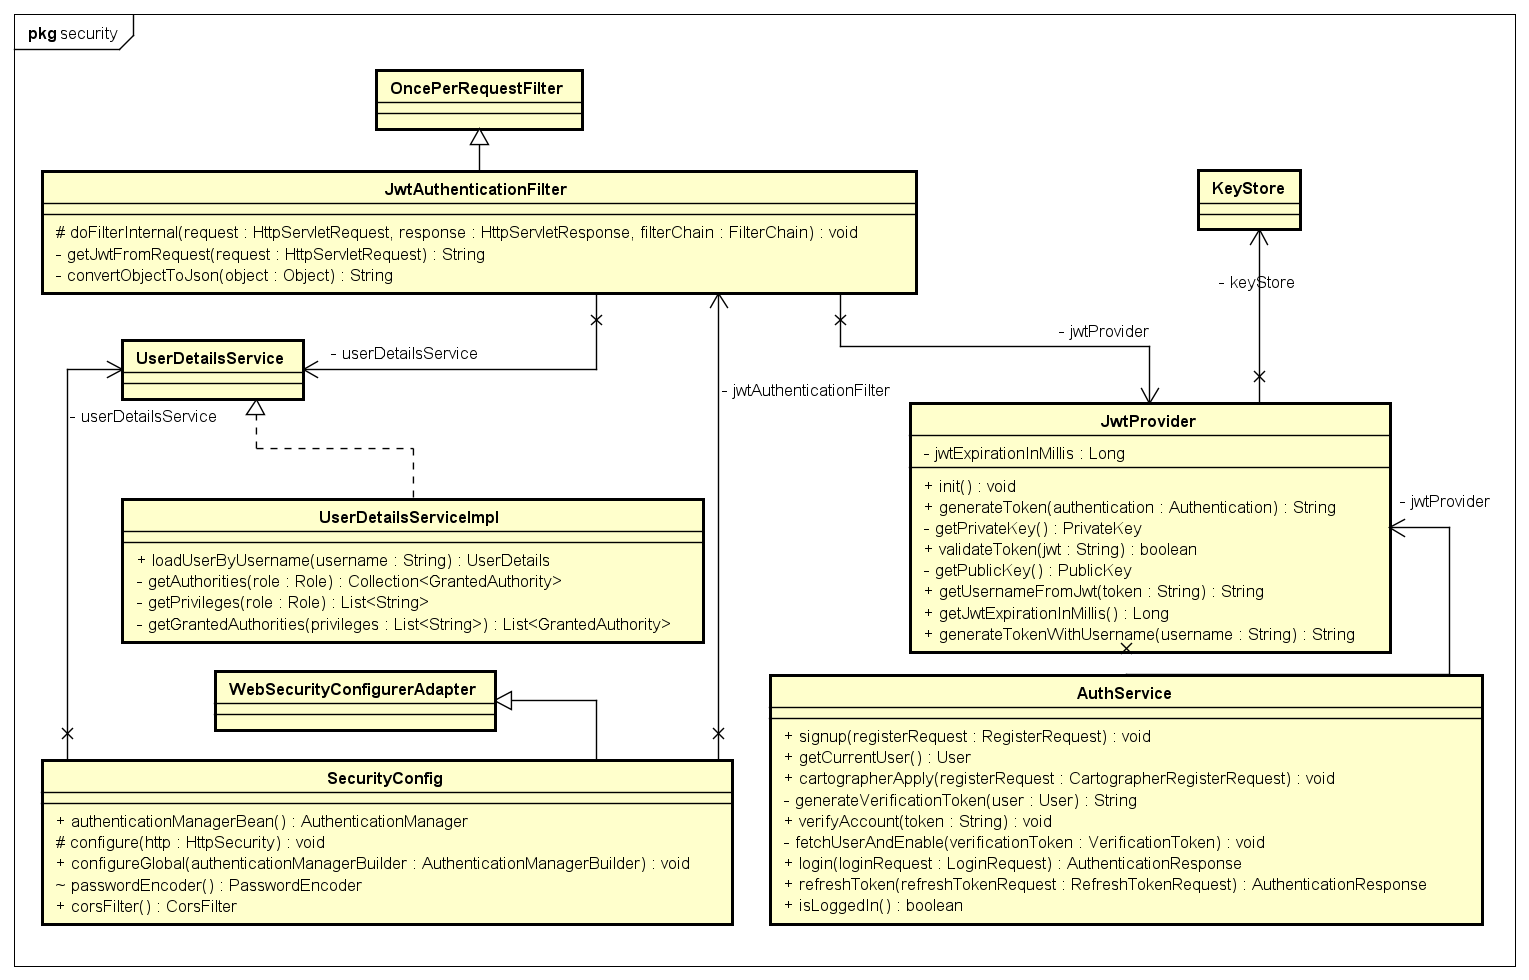
\includegraphics[scale=0.56]{dijagrami/Security_CD} \\
				\caption{Dijagram razreda - Security}
				\label{fig:Security_CD}
			\end{figure}
			
			\textnormal{
				Na slici 4.11. prikazani su još neki dodatni razredi, kao što su konfiguracijski razredi, iznimke i validatori. Iznimke koje se pojave u servisima omataju se SpringGeoFighterException-om koji nasljeđuje RuntimeException. Ako se pogreška propagira iz sustava, možemo provjeriti njezin tip. Ako je zamotana u SpringGeoFighterException, to je iznimka koju smo očekivali, dok u protivnom ukazuje na to da se pojavila neočekivana pogreška u sustavu. U sustavu također postoji i UserInfoInvalidException koji se pojavljuje prilikom zahtjeva s krivim korisničkim podatcima.
			}
		
			\begin{figure}[H]
				\centering
				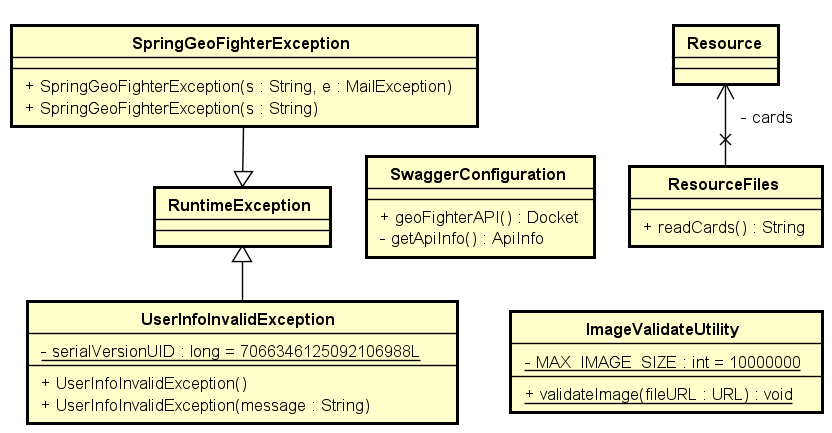
\includegraphics[scale=0.75]{dijagrami/Misc_CD} \\
				\caption{Dijagram razreda - Preostali razredi}
				\label{fig:Misc_CD}
			\end{figure}
			
			\eject
		
		\section{Dijagram stanja}
			
			
			\textbf{\textit{dio 2. revizije}}\\
			
			\textit{Potrebno je priložiti dijagram stanja i opisati ga. Dovoljan je jedan dijagram stanja koji prikazuje \textbf{značajan dio funkcionalnosti} sustava. Na primjer, stanja korisničkog sučelja i tijek korištenja neke ključne funkcionalnosti jesu značajan dio sustava, a registracija i prijava nisu. }
			
			
			\eject 
		
		\section{Dijagram aktivnosti}
			
			\textbf{\textit{dio 2. revizije}}\\
			
			 \textit{Potrebno je priložiti dijagram aktivnosti s pripadajućim opisom. Dijagram aktivnosti treba prikazivati značajan dio sustava.}
			
			\eject
		\section{Dijagram komponenti}
		
			\textbf{\textit{dio 2. revizije}}\\
		
			 \textit{Potrebno je priložiti dijagram komponenti s pripadajućim opisom. Dijagram komponenti treba prikazivati strukturu cijele aplikacije.}
	\chapter{Implementacija i korisničko sučelje}
		
		
		\section{Korištene tehnologije i alati}
		
			\begin{longtabu} to \textwidth {|X[6, l+5]|X[30, 1]|X[20, 2]|}
				
				\hline \multicolumn{3}{|c|}{\textbf{Backend}}	 \\[3pt] \hline
				\endfirsthead
				
				\hline
				\endlastfoot
				
				PostgreSQL13 & \href{https://www.postgresql.org/}{https://www.postgresql.org/}	& Relacijska baza podataka. 	\\ \hline
				
				Java 11 & \href{https://www.oracle.com/java/technologies/javase-jdk11-downloads.html}{https://www.oracle.com/java} & Objektno-orijentirani programski jezik.	\\ \hline
				
				Spring/Spring Boot & \href{https://spring.io/}{https://spring.io/} & Java razvojni okvir. 	\\ \hline
				
				Spring Web MVC  & \href{https://spring.io/guides/gs/serving-web-content/}{https://spring.io/guides/gs/serving-web-content/} & Spring web razvojni okvir.	\\ \hline
				
				Spring Security  & \href{https://spring.io/projects/spring-security}{https://spring.io/projects/spring-security} & 
				Spring razvojni okvir za autentifikacija i autorizaciju. 	\\ \hline
				
				Lombok  & \href{https://projectlombok.org/}{https://projectlombok.org/} & Java library automatizaciju repetitivnog koda. 	\\ \hline
				
				H2  & \href{https://www.h2database.com/}{https://www.h2database.com/} & Relacijska baza podataka korištena za testiranje. 	\\ \hline
				
				SpringFox  & \href{https://springfox.github.io/springfox/}{https://springfox.github.io/springfox/} & Automatizirana JSON API dokumentacija. 	\\ \hline
				
				JWT  & \href{https://jwt.io/}{https://jwt.io/} & URL-sigurno prebacivanje tokena autentifikacije. 	\\ \hline
				
				Apache Commons Validator  & \href{https://commons.apache.org/proper/commons-validator/}{https://commons.apache.org/} & Biblioteka validatora. 	\\ \hline
				
			\end{longtabu}
			
			
			
			\eject
			
			\begin{longtabu} to \textwidth {|X[4, l+3]|X[25, l]|X[20, 2]|}
				
				\hline \multicolumn{3}{|c|}{\textbf{Frontend}}	 \\[3pt] \hline
				\endfirsthead
				
				\hline
				\endlastfoot
				
				Angular & \href{https://angular.io/}{https://angular.io/}	& Radni okvir za izgradnju web aplikacija.	\\ \hline
			
				Bootstrap & \href{https://getbootstrap.com/}{https://getbootstrap.com/} & CSS radni okvir za web development.	\\ \hline
				
				NPM & \href{https://www.npmjs.com/}{https://www.npmjs.com/} & Upravitelj paketa za programski jezik JavasScript.	\\ \hline
				
				Typescript & \href{https://www.typescriptlang.org/}{https://www.typescriptlang.org/} & Programski jezik koji se prevodi u JavaScript.	\\ \hline
				
				Leaflet & \href{https://leafletjs.com/}{https://leafletjs.com/} & Javascript library za izgradnju interaktivnih karata.	\\ \hline
				
				Leaflet Routing Machine & \href{https://www.liedman.net/leaflet-routing-machine/}{https://www.liedman.net/leaflet-routing-machine/} & Javascript library za crtanje ruta nad leafletom.	\\ \hline
				
				Open Source Routing Machine & \href{http://project-osrm.org/}{http://project-osrm.org/} & Servis koji računa rutu između zadanih točaka.	\\ \hline
			\end{longtabu}			
			
			
			\begin{longtabu} to \textwidth {|X[4, l+3]|X[25, l]|X[20, 2]|}
				
				\hline \multicolumn{3}{|c|}{\textbf{Komunikacija i Version Control}}	 \\[3pt] \hline
				\endfirsthead
				
				\hline
				\endlastfoot
				
				Slack & \href{https://slack.com/}{https://slack.com/}	& Platforma za komunikaciju članova.	\\ \hline
				GitLab & \href{https://gitlab.com/}{https://gitlab.com/} & Git Repository manager, issue tracker i CI/CD provider.	\\ \hline
			\end{longtabu}
		
			\begin{longtabu} to \textwidth {|X[4, l+3]|X[25, l]|X[20, 2]|}
				
				\hline \multicolumn{3}{|c|}{\textbf{Web poslužitelj}}	 \\[3pt] \hline
				\endfirsthead
				
				\hline
				\endlastfoot
				
				Heroku & \href{https://www.heroku.com/}{https://www.heroku.com/}	& Cloud platforma za deployanje aplikacija.	\\ \hline
			\end{longtabu}
		
			\begin{longtabu} to \textwidth {|X[4, l+3]|X[30, l]|X[20, 2]|}
				
				\hline \multicolumn{3}{|c|}{\textbf{Web poslužitelj}}	 \\[3pt] \hline
				\endfirsthead
				
				\hline
				\endlastfoot
				
				IntelliJ IDEA & \href{https://www.jetbrains.com/idea/}{https://www.jetbrains.com/idea/}	& JAVA IDE.	\\ \hline
				
				WebStorm & \href{https://www.jetbrains.com/webstorm/}{https://www.jetbrains.com/webstorm/}	& JavaScript IDE.	\\ \hline
			\end{longtabu}
			
			
			\eject 
		
	
		\section{Ispitivanje programskog rješenja}
						
			\subsection{Ispitivanje komponenti}
			\textit{Za potrebe testiranja naših Spring backend komponenti koristili smo JUnit testing framework. JUnit nam omogućuje pisanje testova koji se jako brzo izvode pomoću njegovog Mockito frameworka tako da nije potrebno pokrenuti cijelu Spring aplikaciju već možemo falsificirati odgovore nekih metoda koje bi inače razgovarale s bazom. Uz te testove (8-10) napisali smo i integracijske testove (1-6) u kojima koristimo MockMvc kojim simuliramo HTTP zahtjeve na našu backend poslužitelj i na temelju dobivenih HTTP odgovora ispitivamo njihovu ispravnost. Ti testovi zahtijevaju potpuno pokretanje Spring aplikacije te su nešto sporiji. Također napisali smo nekoliko standardnih testova koji ispituju statičke metode. Napisan je i jedan test koji poziva ne-implementiranu funkcionalnost dok ona baca UnsupportedOeprationException, ali on nije prikazan u primjerima ispod i u programskom je kodu anotacijom onemogućen. Takav test faila pri pokretanju. Od svih testova implementiranih funkcionalnosti prolaze svi i to je vidljivo na slici koja se nalazi na dnu poglavlja.}
			
			\subsubsection{Test 1: Uspješna registracija u sustav}
			Korisnik se registrira u sustav e-mail adresom, korisničkim imenom, lozinkom i URL-om svoje slike. \\
			U ovom testu su svi podatci ispravni, pa stoga poslužitelj treba uspješno izvršiti registraciju korisnika i vratiti statusni kod 200 OK.
			
			\begin{figure}[H]
				\centering
				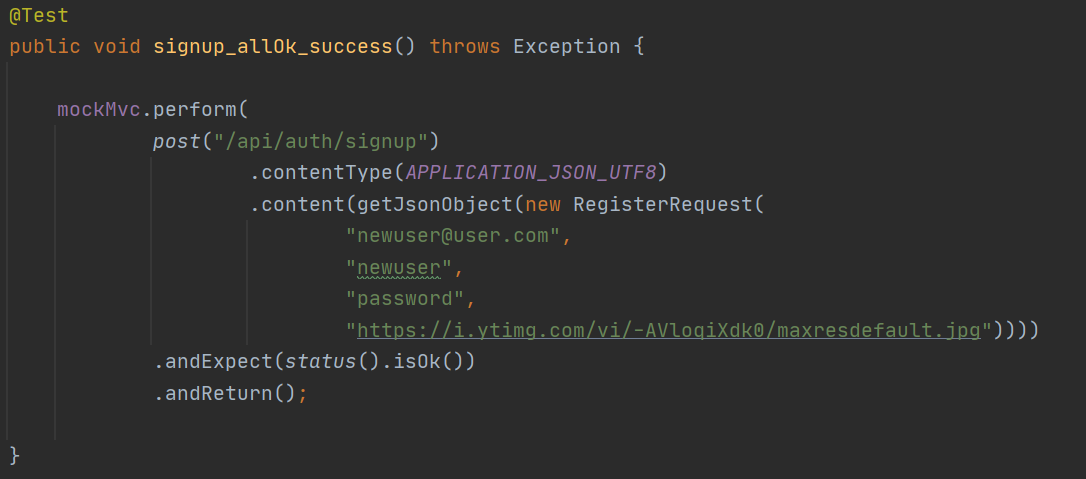
\includegraphics[scale=0.75]{slike/test1} \\
				\caption{ Test registracije u sustav ispravnim podacima}
				\label{fig:test1}
			\end{figure}
		
		
			\subsubsection{Test 2: Neuspješna registracija u sustav radi zauzetog korisničkog imena}
			Korisnik se pokuša registrirati u sustav imenom koje je zauzeto. \\
			Poslužitelj javlja da registracija nije uspjela,
			a klijentu se prikazuje tost koji se pojavljuje u gornjem desnom kutu ekrana.
			
			\begin{figure}[H]
				\centering
				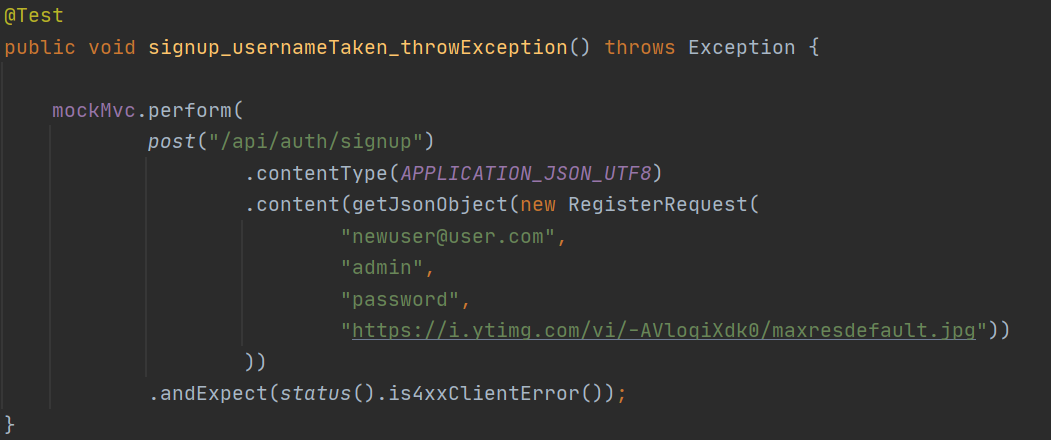
\includegraphics[scale=0.75]{slike/test2} \\
				\caption{ Test registracije u sustav zauzetim korisničkim imenom}
				\label{fig:test2}
			\end{figure}
		
			\subsubsection{Test 3: Neuspješna registracija u sustav radi lošeg URL-a slike}
			Korisnik se pokuša registrirati u sustav URL-om svoje slike koji je možda ispravno napisan, ali slika s tim URL-om nije dohvatljiva. \\
			Poslužitelj javlja da registracija nije uspjela, a klijentu se prikazuje tost koji se pojavljuje u gornjem desnom kutu ekrana.
			
			\begin{figure}[H]
				\centering
				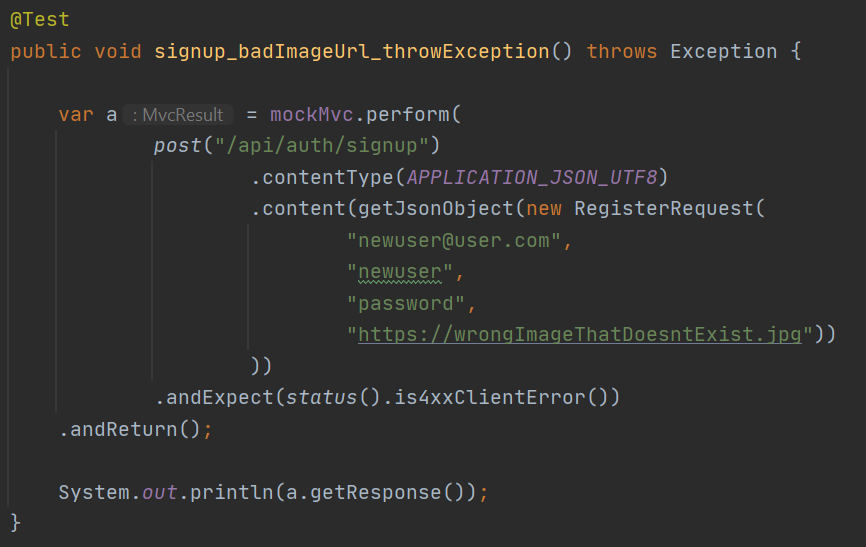
\includegraphics[scale=0.75]{slike/test3} \\
				\caption{ Test registracije u sustav lošim URL-om slike}
				\label{fig:test3}
			\end{figure}
		
			\subsubsection{Test 4: Uspješna prijava za kartografa}
			Korisnik se prijavljuje za kartografa u sustav IBAN brojem računa i URL-slikom svoje osobne iskaznice. \\
			U ovom testu su svi podatci ispravni, pa stoga poslužitelj treba uspješno pohraniti prijavu korisnika za kartografa i vratiti statusni kod 200 OK.
			
			\begin{figure}[H]
				\centering
				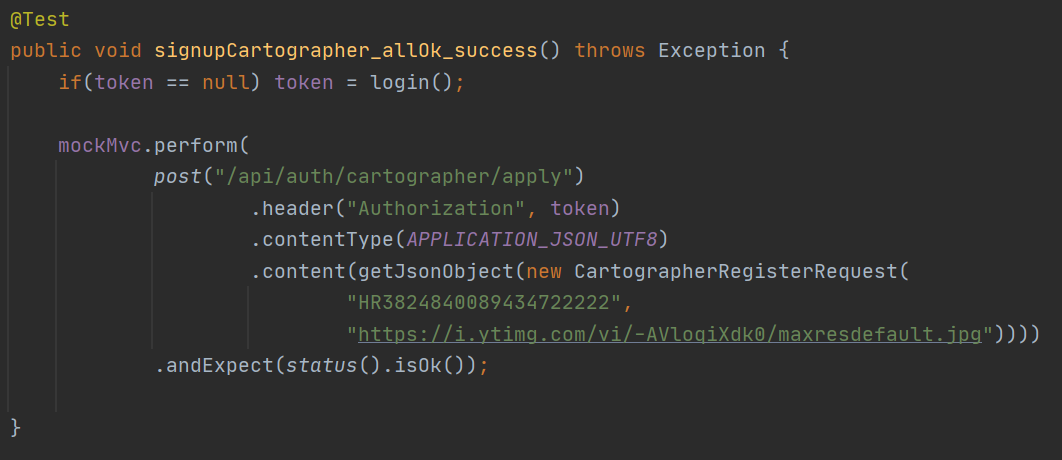
\includegraphics[scale=0.75]{slike/test4} \\
				\caption{ Test prijave za kartografa ispravnim podacima}
				\label{fig:test4}
			\end{figure}
		
			\subsubsection{Test 5: Uspješna prijava u sustav}
			Korisnik se prijavljuje u sustav korisničkim imenom i lozinkom. \\
			U ovom testu su svi podatci ispravni, pa stoga poslužitelj treba uspješno izvršiti prijavu korisnika i vratiti statusni kod 200 OK.
			
			\begin{figure}[H]
				\centering
				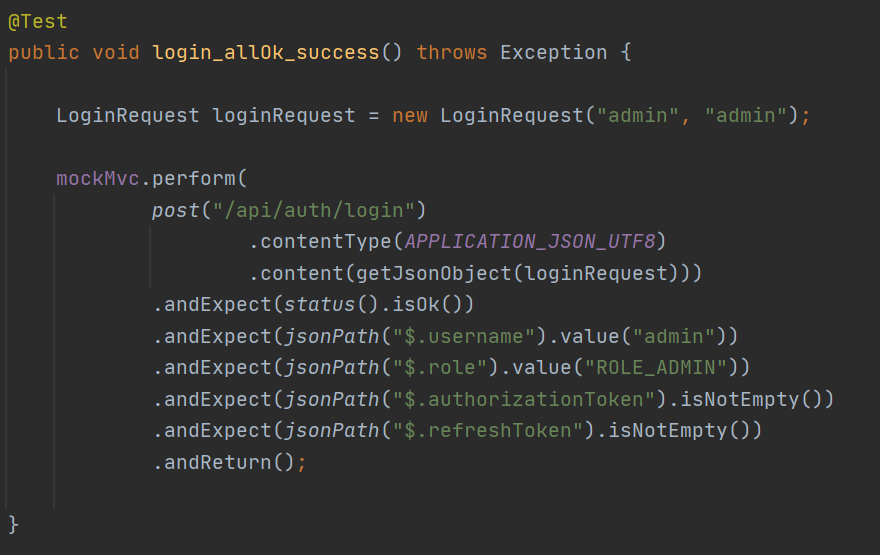
\includegraphics[scale=0.75]{slike/test5} \\
				\caption{ Test prijave u sustav ispravnim podacima}
				\label{fig:test5}
			\end{figure}
		
			\subsubsection{Test 6: Neuspješna prijava u sustav radi neispravnih podataka}
			Korisnik se pokuša prijaviti u sustav s neispravnom kombinacijom korisničkog imena i lozinke. \\
			Poslužitelj baca iznimku tipa BadCredentialsException a klijentu javlja da prijava nije uspjela.
			
			\begin{figure}[H]
				\centering
				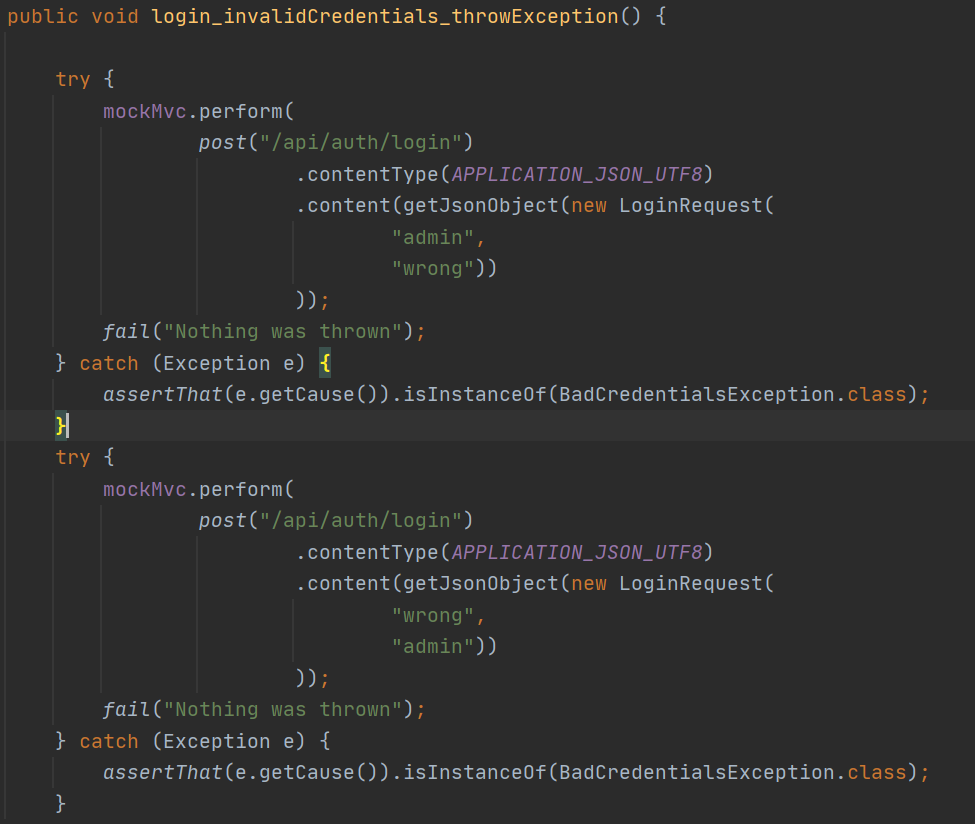
\includegraphics[scale=0.75]{slike/test6} \\
				\caption{ Test prijave u sustav neispravnim podacima}
				\label{fig:test6}
			\end{figure}
		
			\eject
		
			\subsubsection{Test 7: Parsiranje i ispisivanje koordinata}
			Ispitivanje metode koja parsira String u Point2D.Double u kojem čuvamo lokacije. \\
			Također ispitivanje da se lokacija iz klase Point2D.Double dobro ispisuje kao string.
		
			\begin{figure}[H]
				\centering
				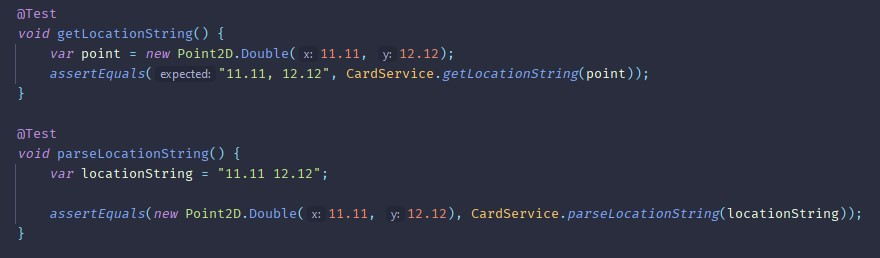
\includegraphics[scale=0.65]{slike/test7} \\
				\caption{ Test parsiranja i pretvaranje lokaciju u String }
				\label{fig:test7}
			\end{figure}
		
			\subsubsection{Test 8: Osvajanje karte ne radi ako je igrač predaleko od nje}
			Ispitivanje metode koja se poziva prilikom osvajanja karte i očekivanje da će baciti exception koji znači da se karta nije mogla osvojiti zbog udaljenosti od igrača.
			
			\begin{figure}[H]
				\centering
				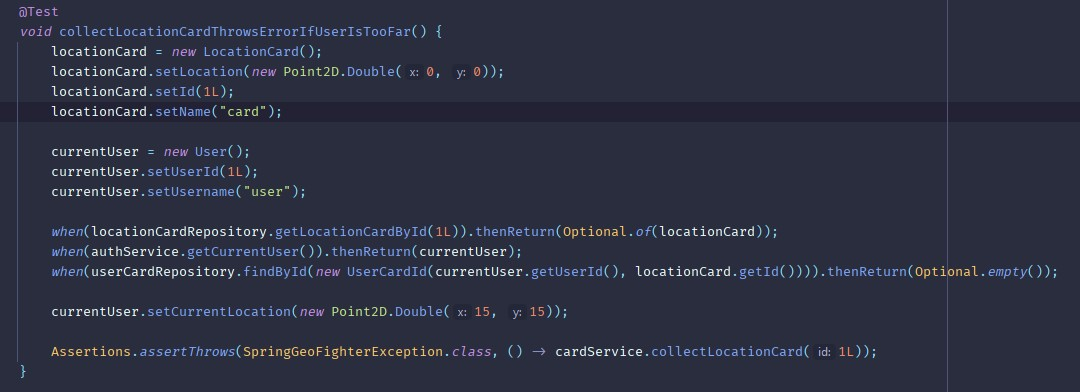
\includegraphics[scale=0.55]{slike/test8} \\
				\caption{ Test osvajanja karte koji baca exception ako je igrač predaleko }
				\label{fig:test8}
			\end{figure}
		
			\subsubsection{Test 9: Osvajanje karte ne radi ništa ako je igrač već ima}
			Ispitivanje metode koja se poziva prilikom osvajanja karte i očekivanje da ona neće napraviti nikakvu akciju spremanja u bazu podataka ukoliko igrač koji pokušava osvojiti kartu nju već posjeduje.
			
			\begin{figure}[H]
				\centering
				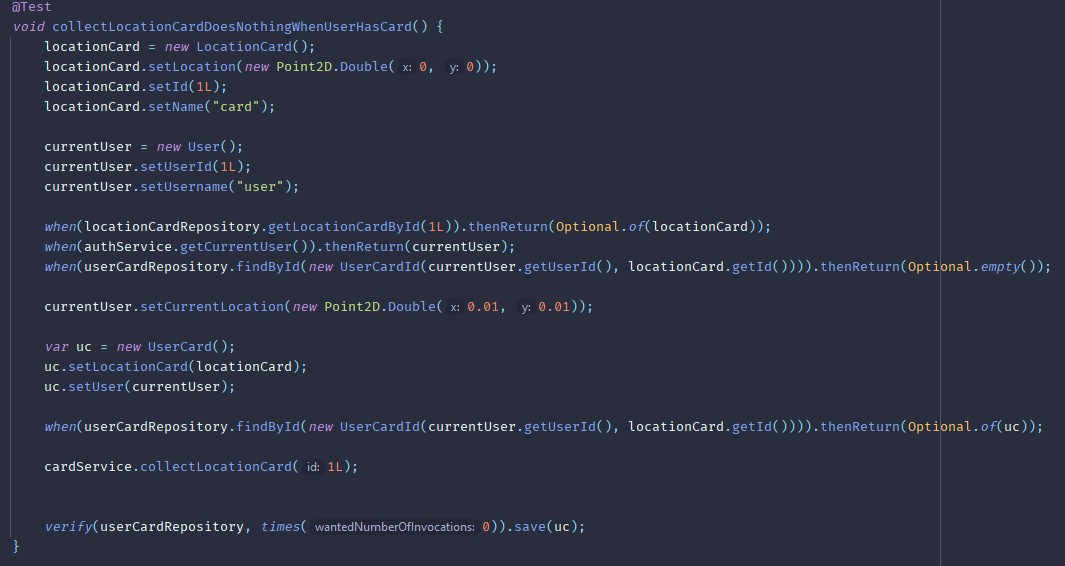
\includegraphics[scale=0.55]{slike/test9} \\
				\caption{ Test osvajanja karte koji provjerava da se ne poziva spremanje u bazu ako igrač posjeduje kartu}
				\label{fig:test9}
			\end{figure}
		
			\subsubsection{Test 10: Osvajanje karte uspješno sprema kartu}
			Ispitivanje metode uspješnog spremanja relacije karta-igrač u bazu podataka kod njenog osvajanja.
			
			\begin{figure}[H]
				\centering
				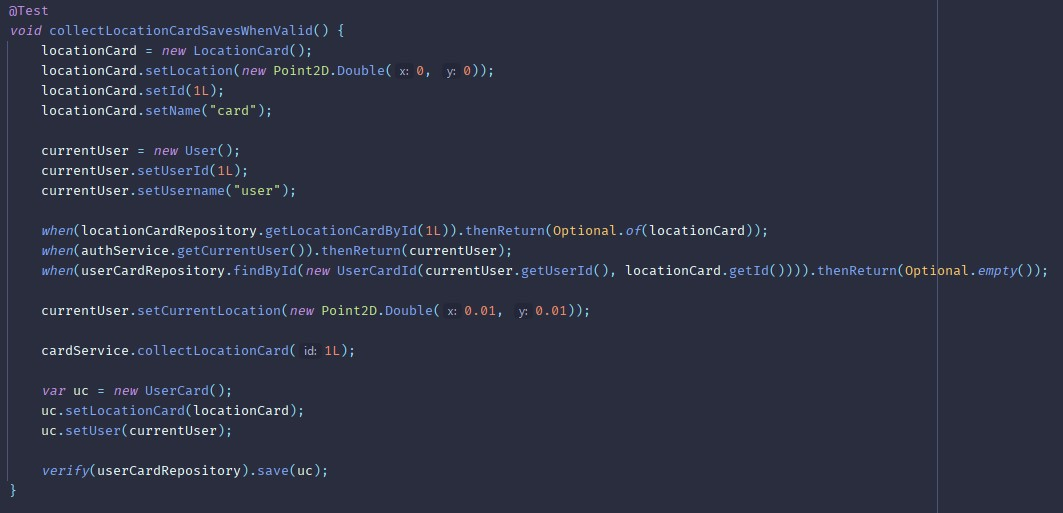
\includegraphics[scale=0.55]{slike/test10} \\
				\caption{ Test uspješnog spremanja u bazu podataka kod osvajanja}
				\label{fig:test10}
			\end{figure}
		
			\subsubsection{Test 11: Test računanja daljine između dvije lokacije}
			Ispitivanje metode koja računa zračnu udaljenost između svije geografske lokacije.
			Lokacija se uspoređuje s poznatom udaljenosti u kilometrima između neke dvije točke.
			
			\begin{figure}[H]
				\centering
				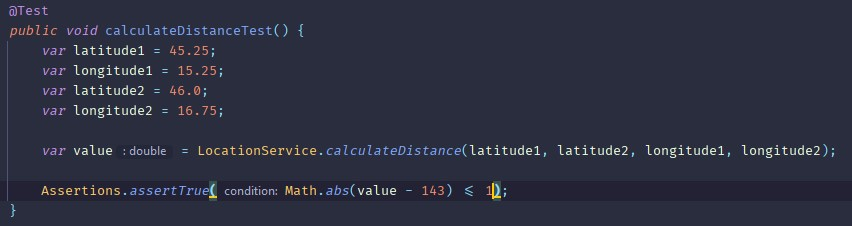
\includegraphics[scale=0.70]{slike/test11} \\
				\caption{ Test uspješnog spremanja u bazu podataka kod osvajanja}
				\label{fig:test10}
			\end{figure}
			
			\begin{figure}[H]
				\centering
				
\includegraphics[scale=1]{slike/ishodTestova} \\
				\caption{ Rezultati izvođenja svih napisanih testova}
				\label{fig:ishodTestova}
			\end{figure}
			
			\eject
			
			\subsection{Ispitivanje sustava}
			
		    Za potrebe ispitivanja sustava, koristili smo Selenium IDE.
			\subsubsection{Test 1: Registracija korisnika}
			\textbf{Očekivano: } Klikom na gumb \textit{Sign Up} učitava se stranica s formom za unos podataka potrebnih za registraciju korisnika: \textit{e-mail adresa, korisničko ime, zaporka} te \textit{poveznica na sliku profila}.\\
			\textbf{Rezultat: } Korisnik  je  uspješno  registriran  u  bazu  podataka  ili  je  sustav  dojavio grešku.\\
			
			    Na slici 5.13. prikazana je poruka prilikom neuspješne registracije korisnika u sustav. Na slici 5.14. prikazan je uspješan test registracije u alatu Selenium.

			\begin{figure}[H]
				\centering
				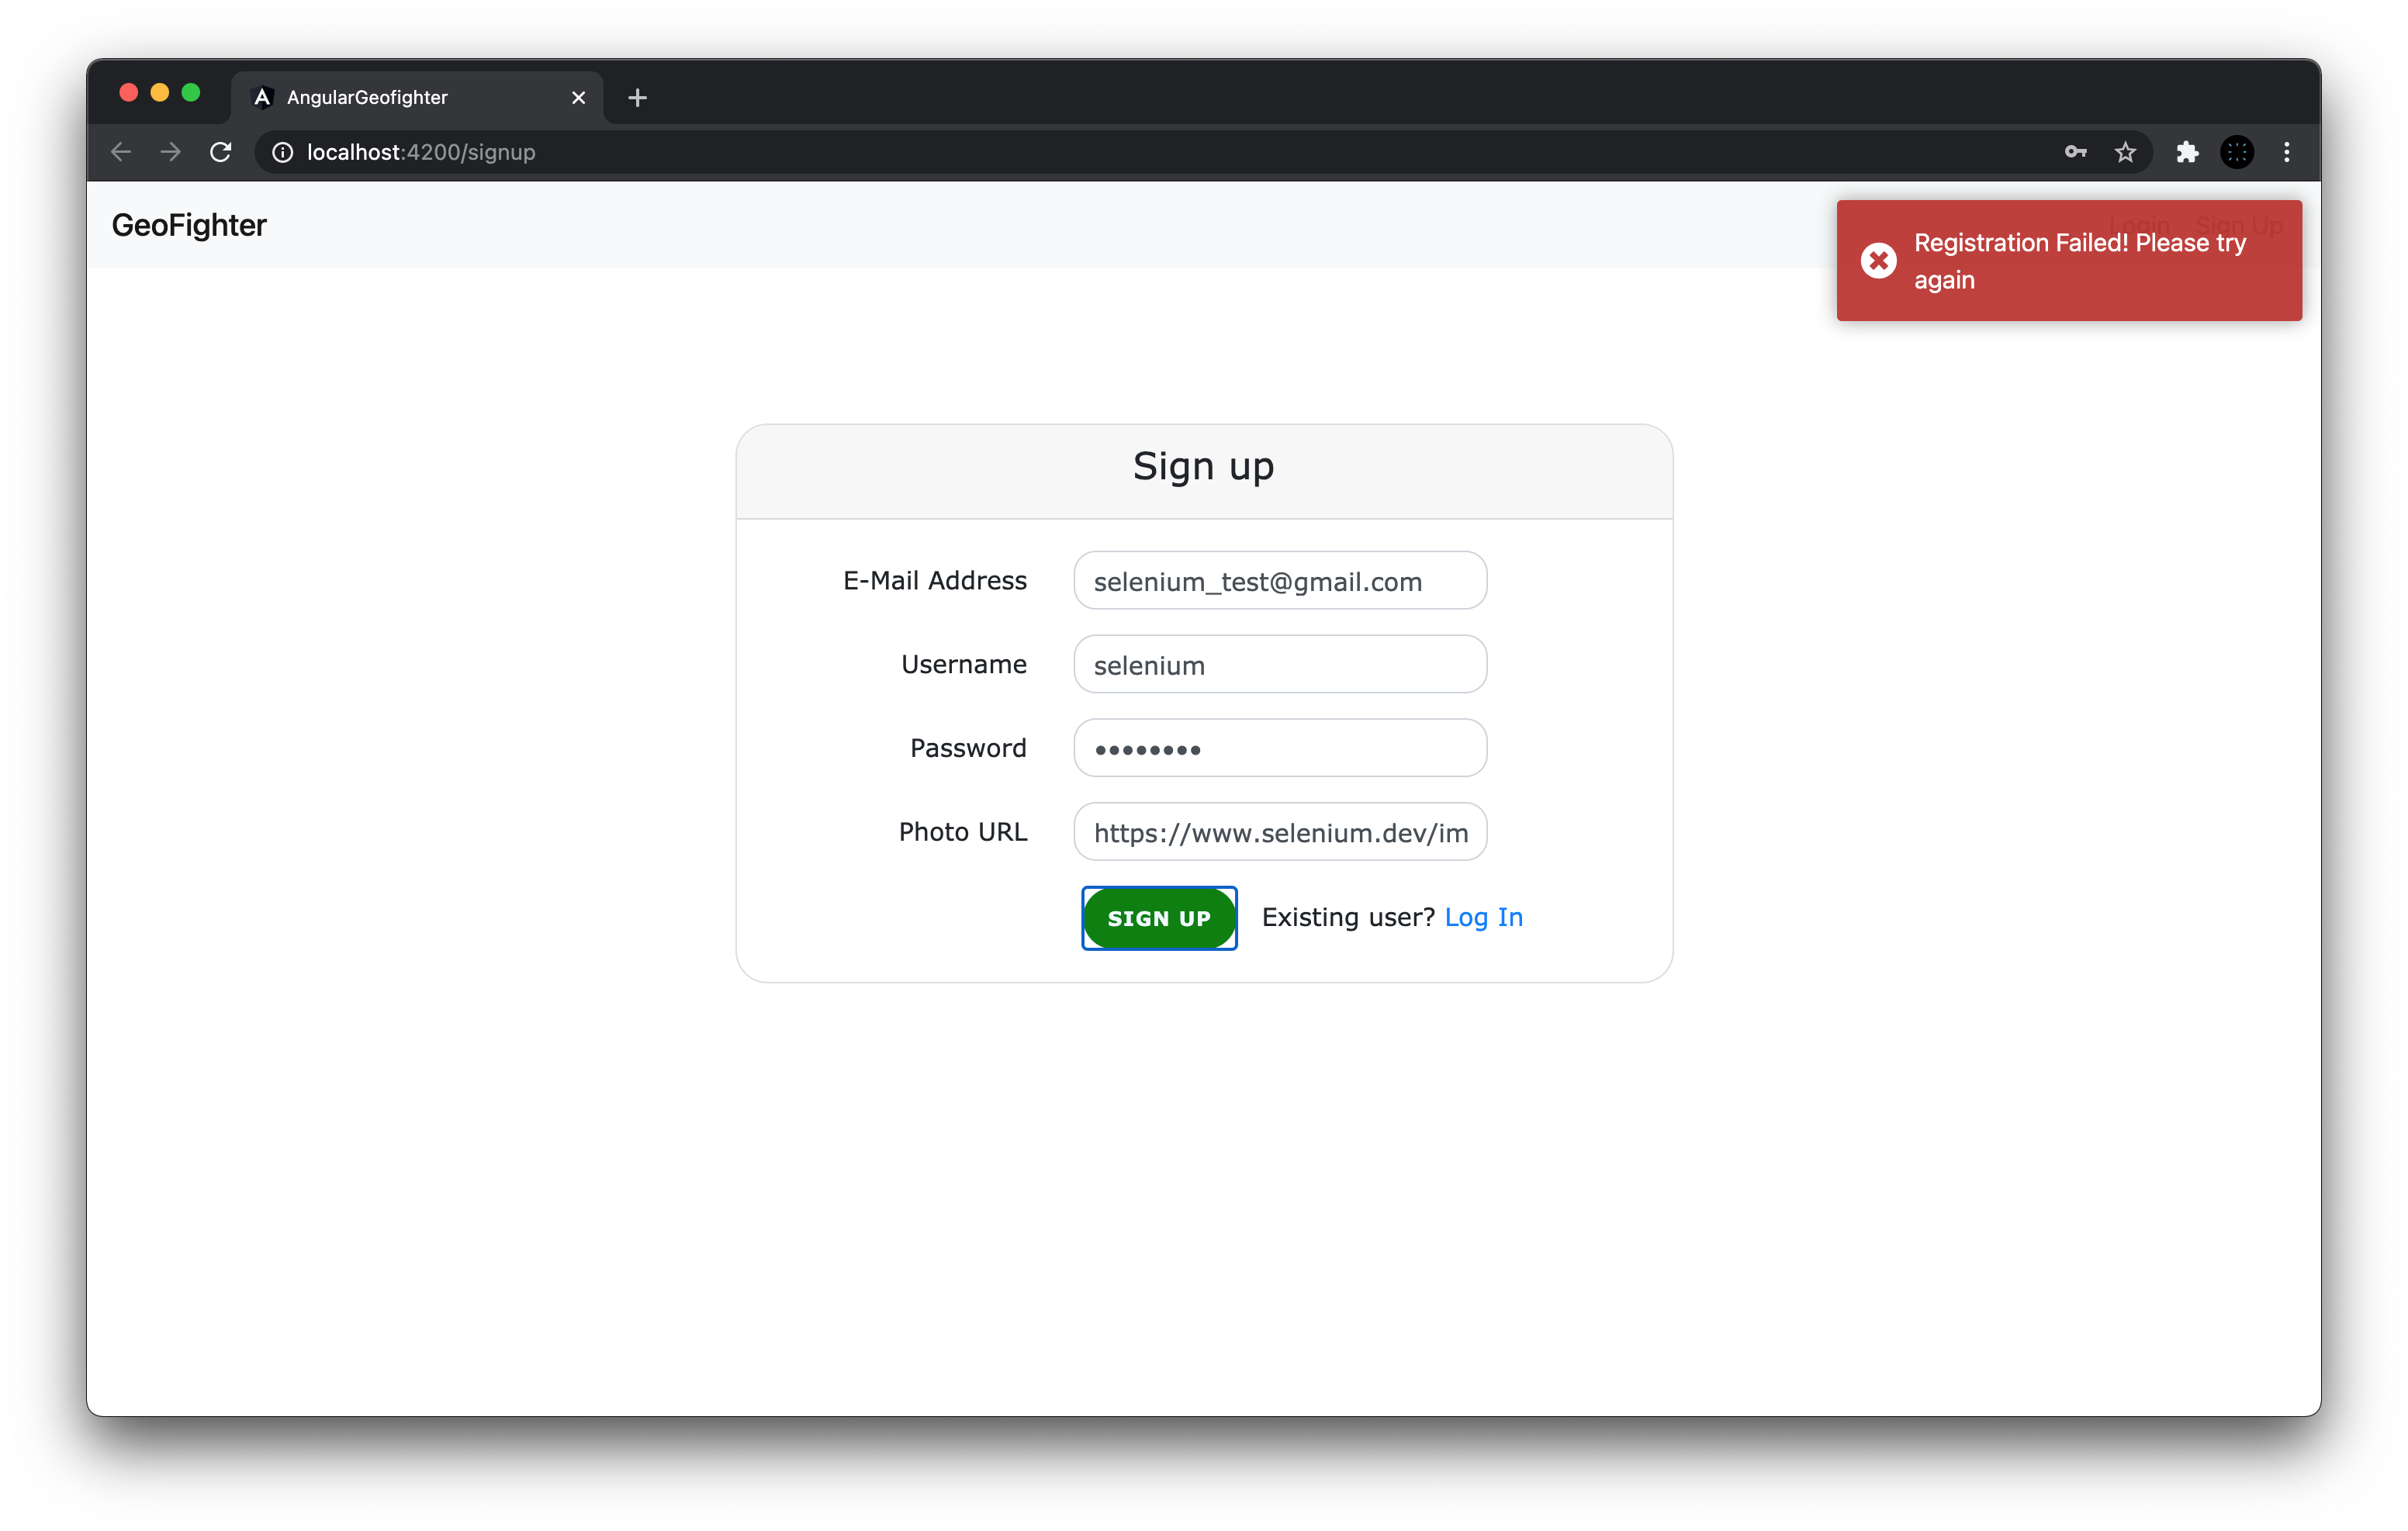
\includegraphics[scale=0.27]{slike/SeleniumRegistrationFail.png} \\
				\caption{ Prikaz poruke za neispravnu registraciju}
				\label{fig:SeleniumRegistrationFail}
			\end{figure}

			\begin{figure}[H]
				\centering
				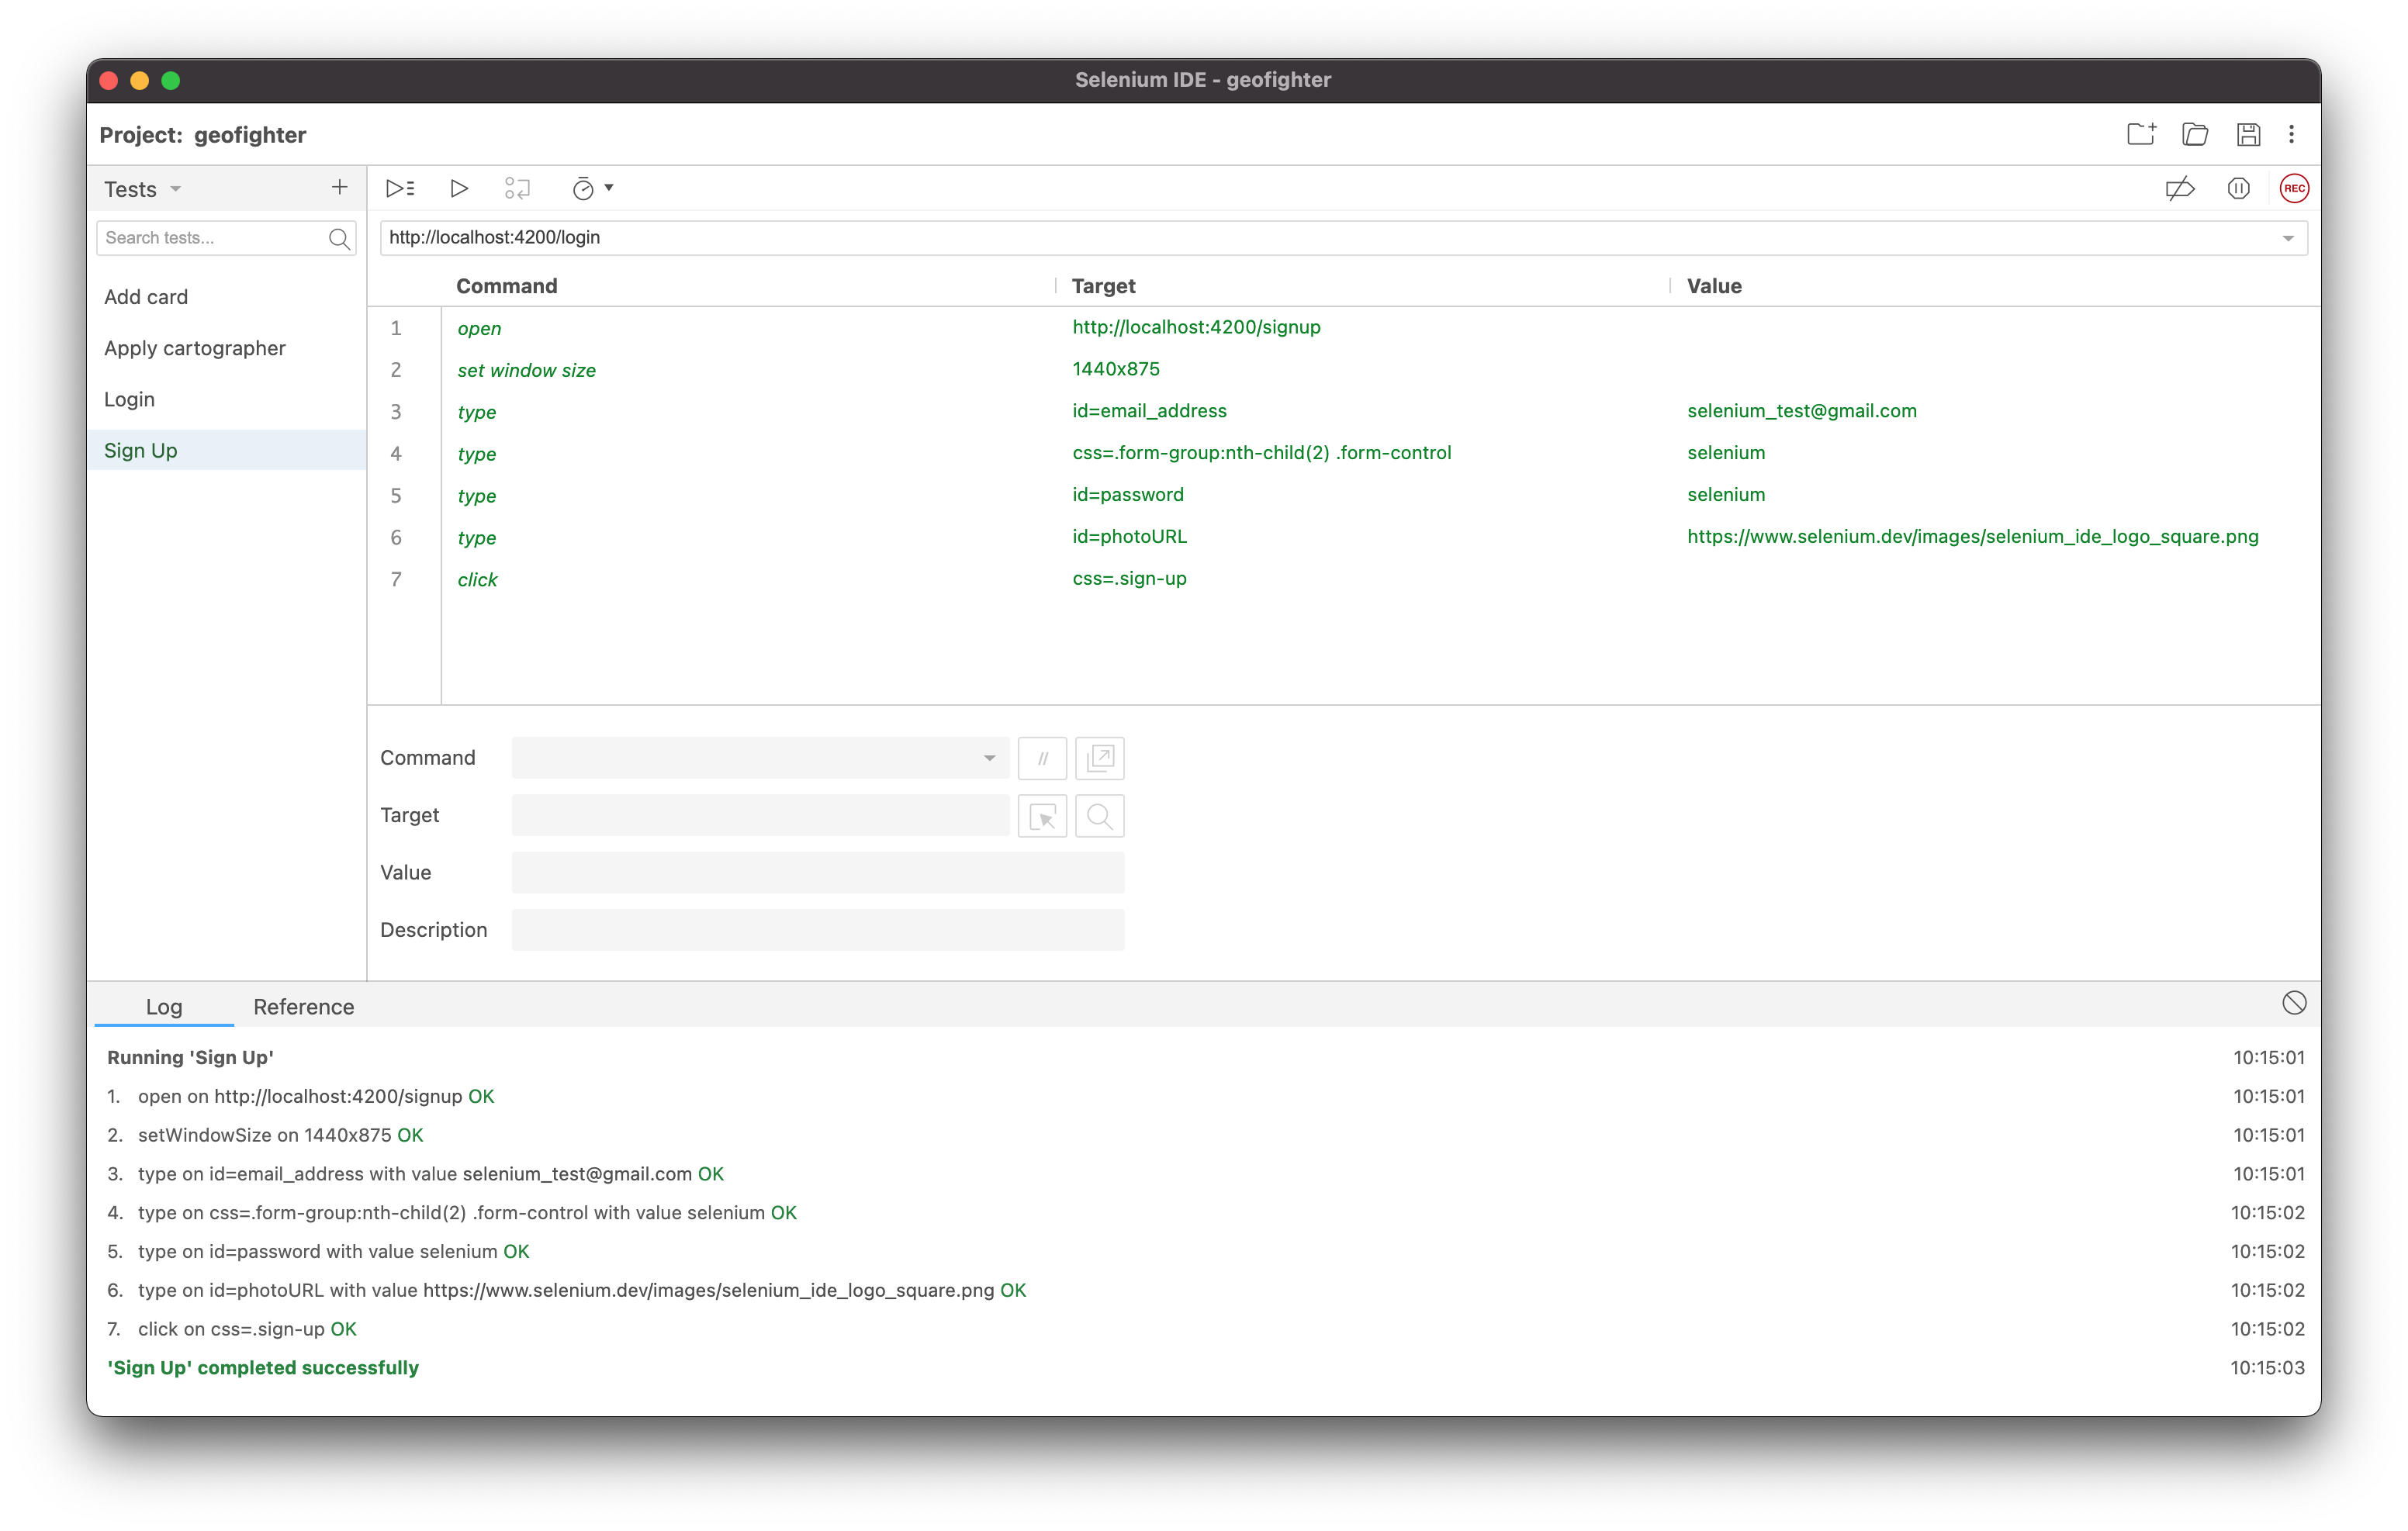
\includegraphics[scale=0.27]{slike/SeleniumRegistrationTest.png} \\
				\caption{ Selenium test koji prikazuje ispravnu registraciju}
				\label{fig:SeleniumRegistrationTest}
			\end{figure}

			\subsubsection{Test 2: Prijava korisnika u aplikaciju}
			\textbf{Očekivano: } Klikom na gumb \textit{Login} učitava se stranica s formom za unos podataka potrebnih za prijavu korisnika u aplikaciju: \textit{korisničko ime} i \textit{lozinka}.\\
			\textbf{Rezultat: } Korisnik  je  uspješno  prijavljen u aplikaciju ili  je  sustav  dojavio grešku.\\

			    Na slici 5.15. prikazan je prozor unutar aplikacije nakon uspješne prijave u aplikaciju. Na slici 5.16. prikazan je uspješan test prijave u aplikaciju u alatu Selenium.

			\begin{figure}[H]
				\centering
				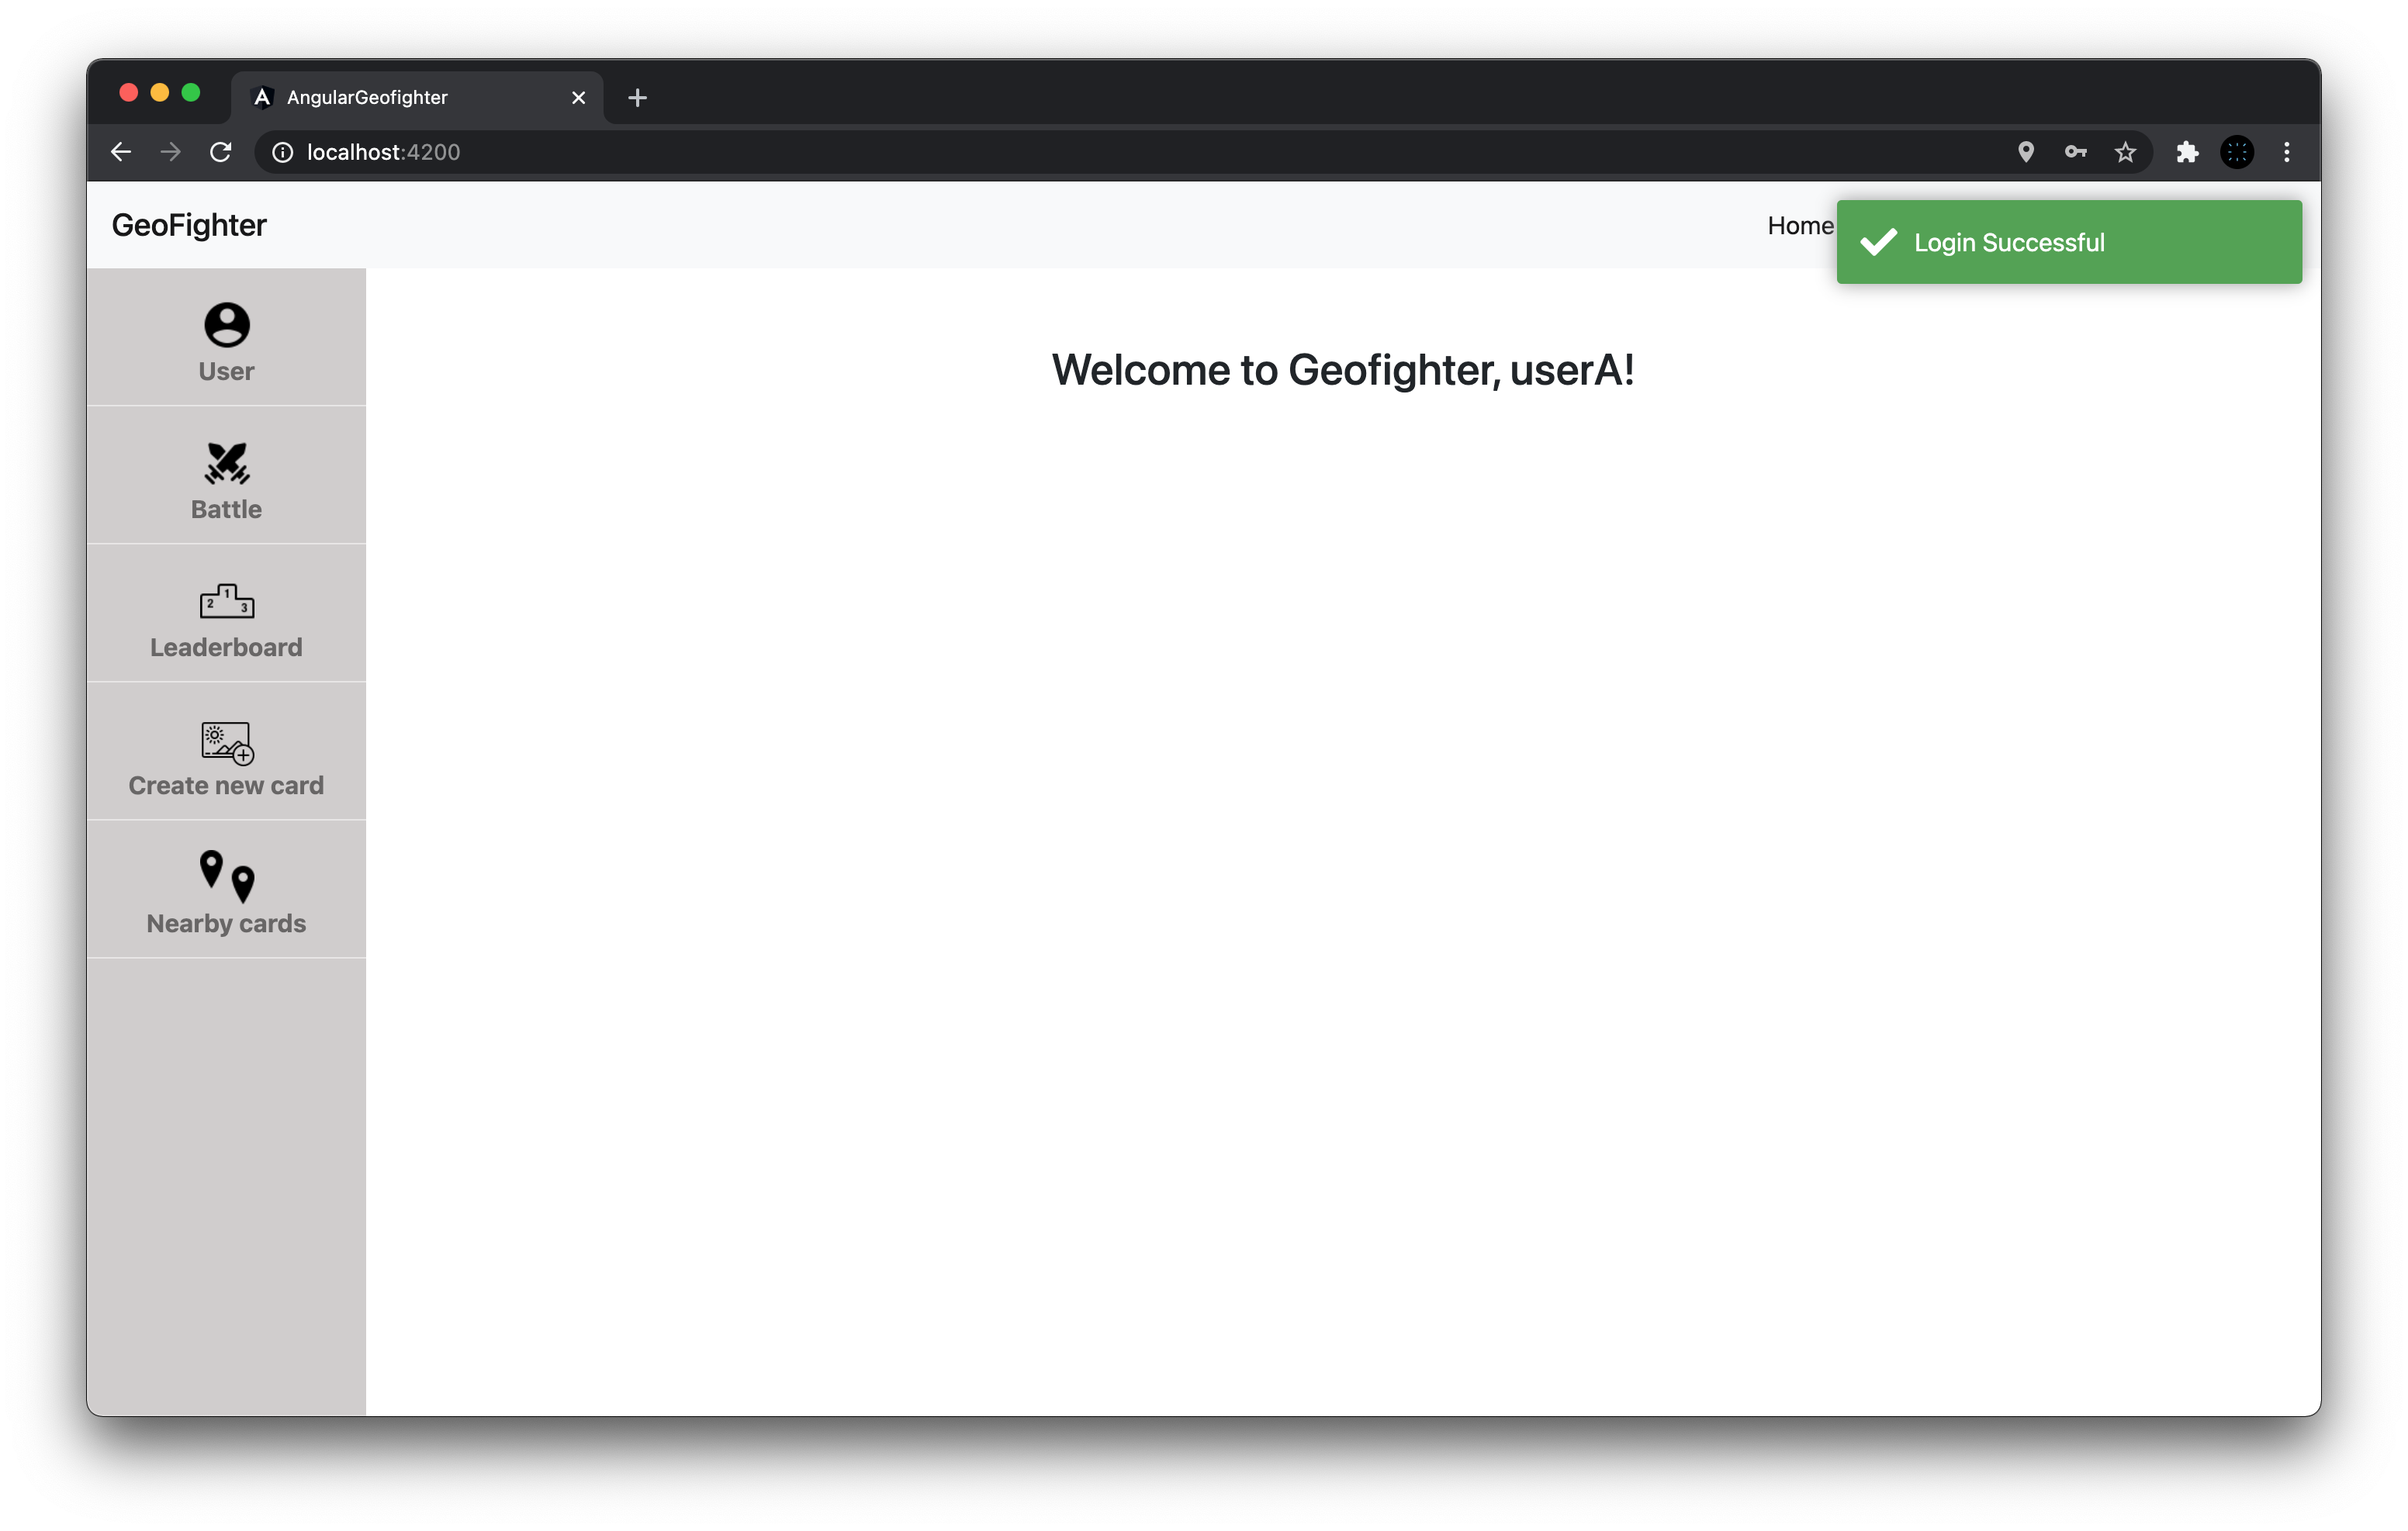
\includegraphics[scale=0.27]{slike/SeleniumLoginSuccess.png} \\
				\caption{ Prozor nakon uspješne prijave u aplikaciju}
				\label{fig:SeleniumLoginSuccess}
			\end{figure}

			\begin{figure}[H]
				\centering
				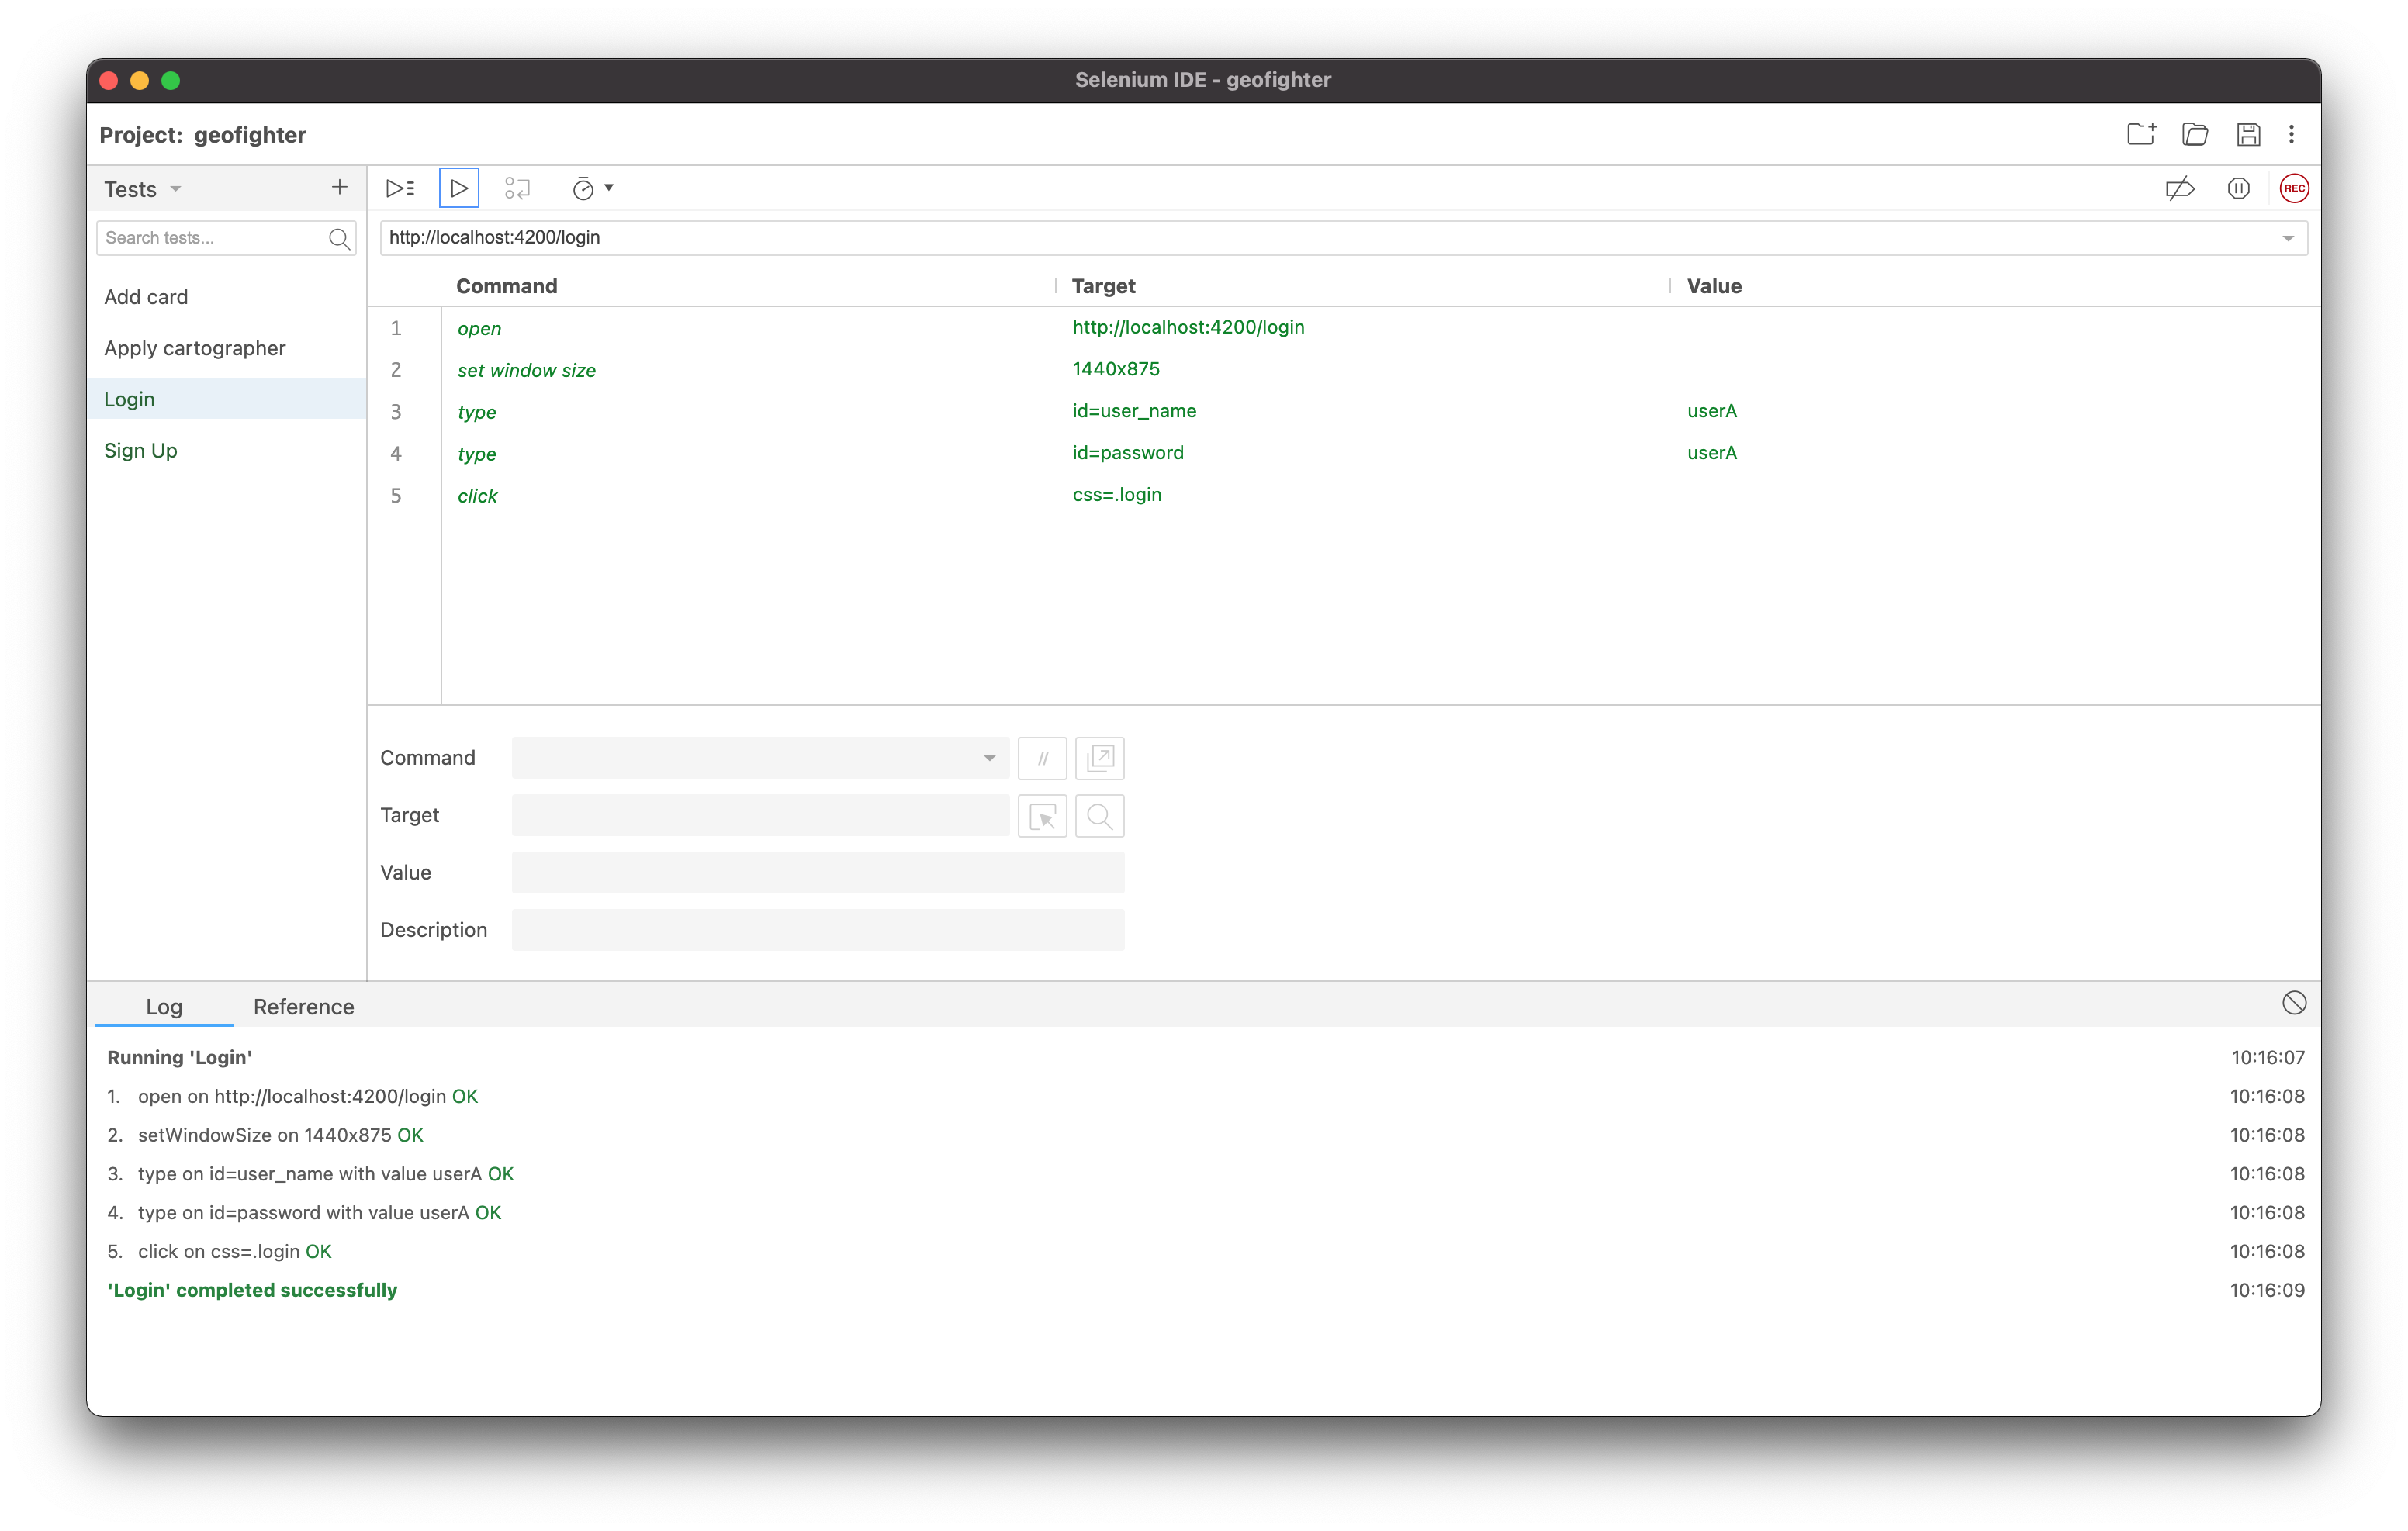
\includegraphics[scale=0.27]{slike/SeleniumLoginTest.png} \\
				\caption{ Selenium test koji prikazuje ispravnu prijavu u aplikaciju}
				\label{fig:SeleniumRegistrationFail}
			\end{figure}

			\subsubsection{Test 3: Prijava korisnika za poziciju kartografa}
			\textbf{Očekivano: } Nakon uspješne prijave korisnika u aplikaciju i nakon što korisnik stisne gumb \textit{Cartographer Apply} učitava se stranica s formom za unos podataka potrebnih za prijavu korisnika za poziciju kartografa: \textit{IBAN} i \textit{poveznica na sliku osobnog dokumenta}.\\
			\textbf{Rezultat: } Korisnik  se uspješno prijavio za poziciju kartografa ili  je  sustav  dojavio grešku.\\

			    Na slici 5.17. prikazana je poruka uspješne prijave za poziciju kartografa. Na slici 5.18. prikazan je uspješan test prijave za poziciju kartografa u alatu Selenium.

			\begin{figure}[H]
				\centering
				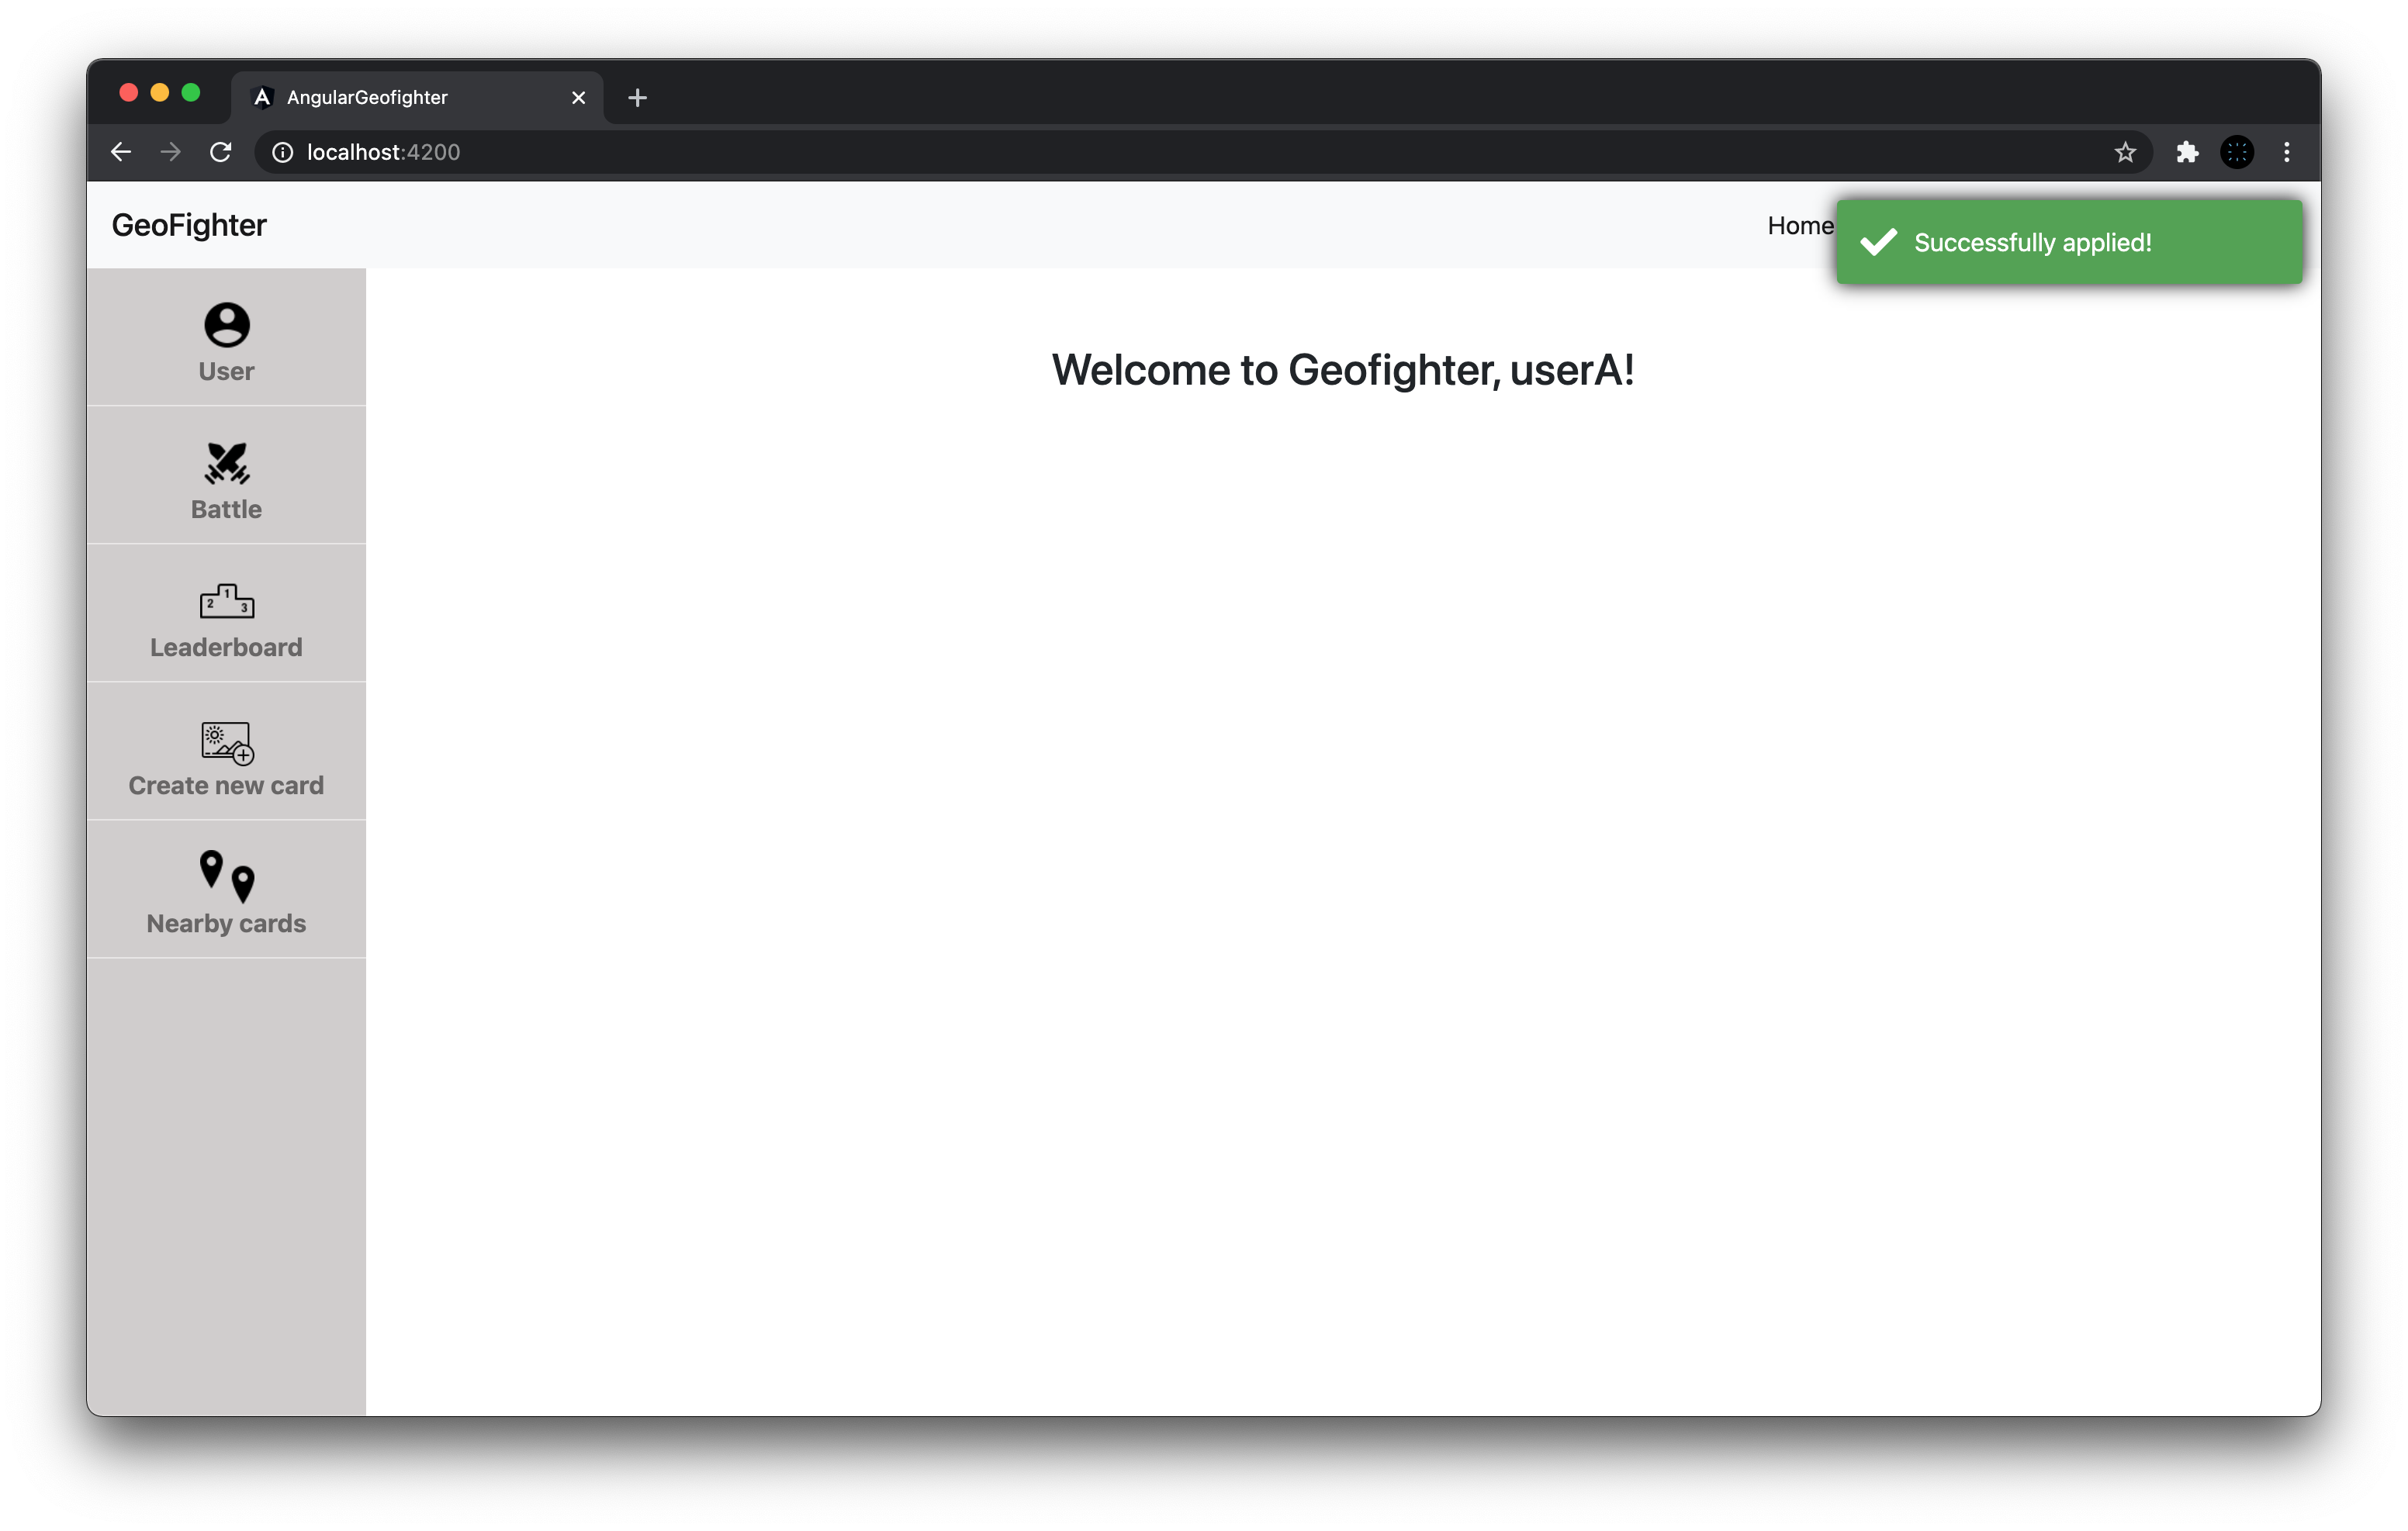
\includegraphics[scale=0.27]{slike/SeleniumCartographerSuccess.png} \\
				\caption{ Prozor nakon uspješne prijave korisnika za poziciju kartografa}
				\label{fig:SeleniumCartographerSuccess}
			\end{figure}

			\begin{figure}[H]
				\centering
				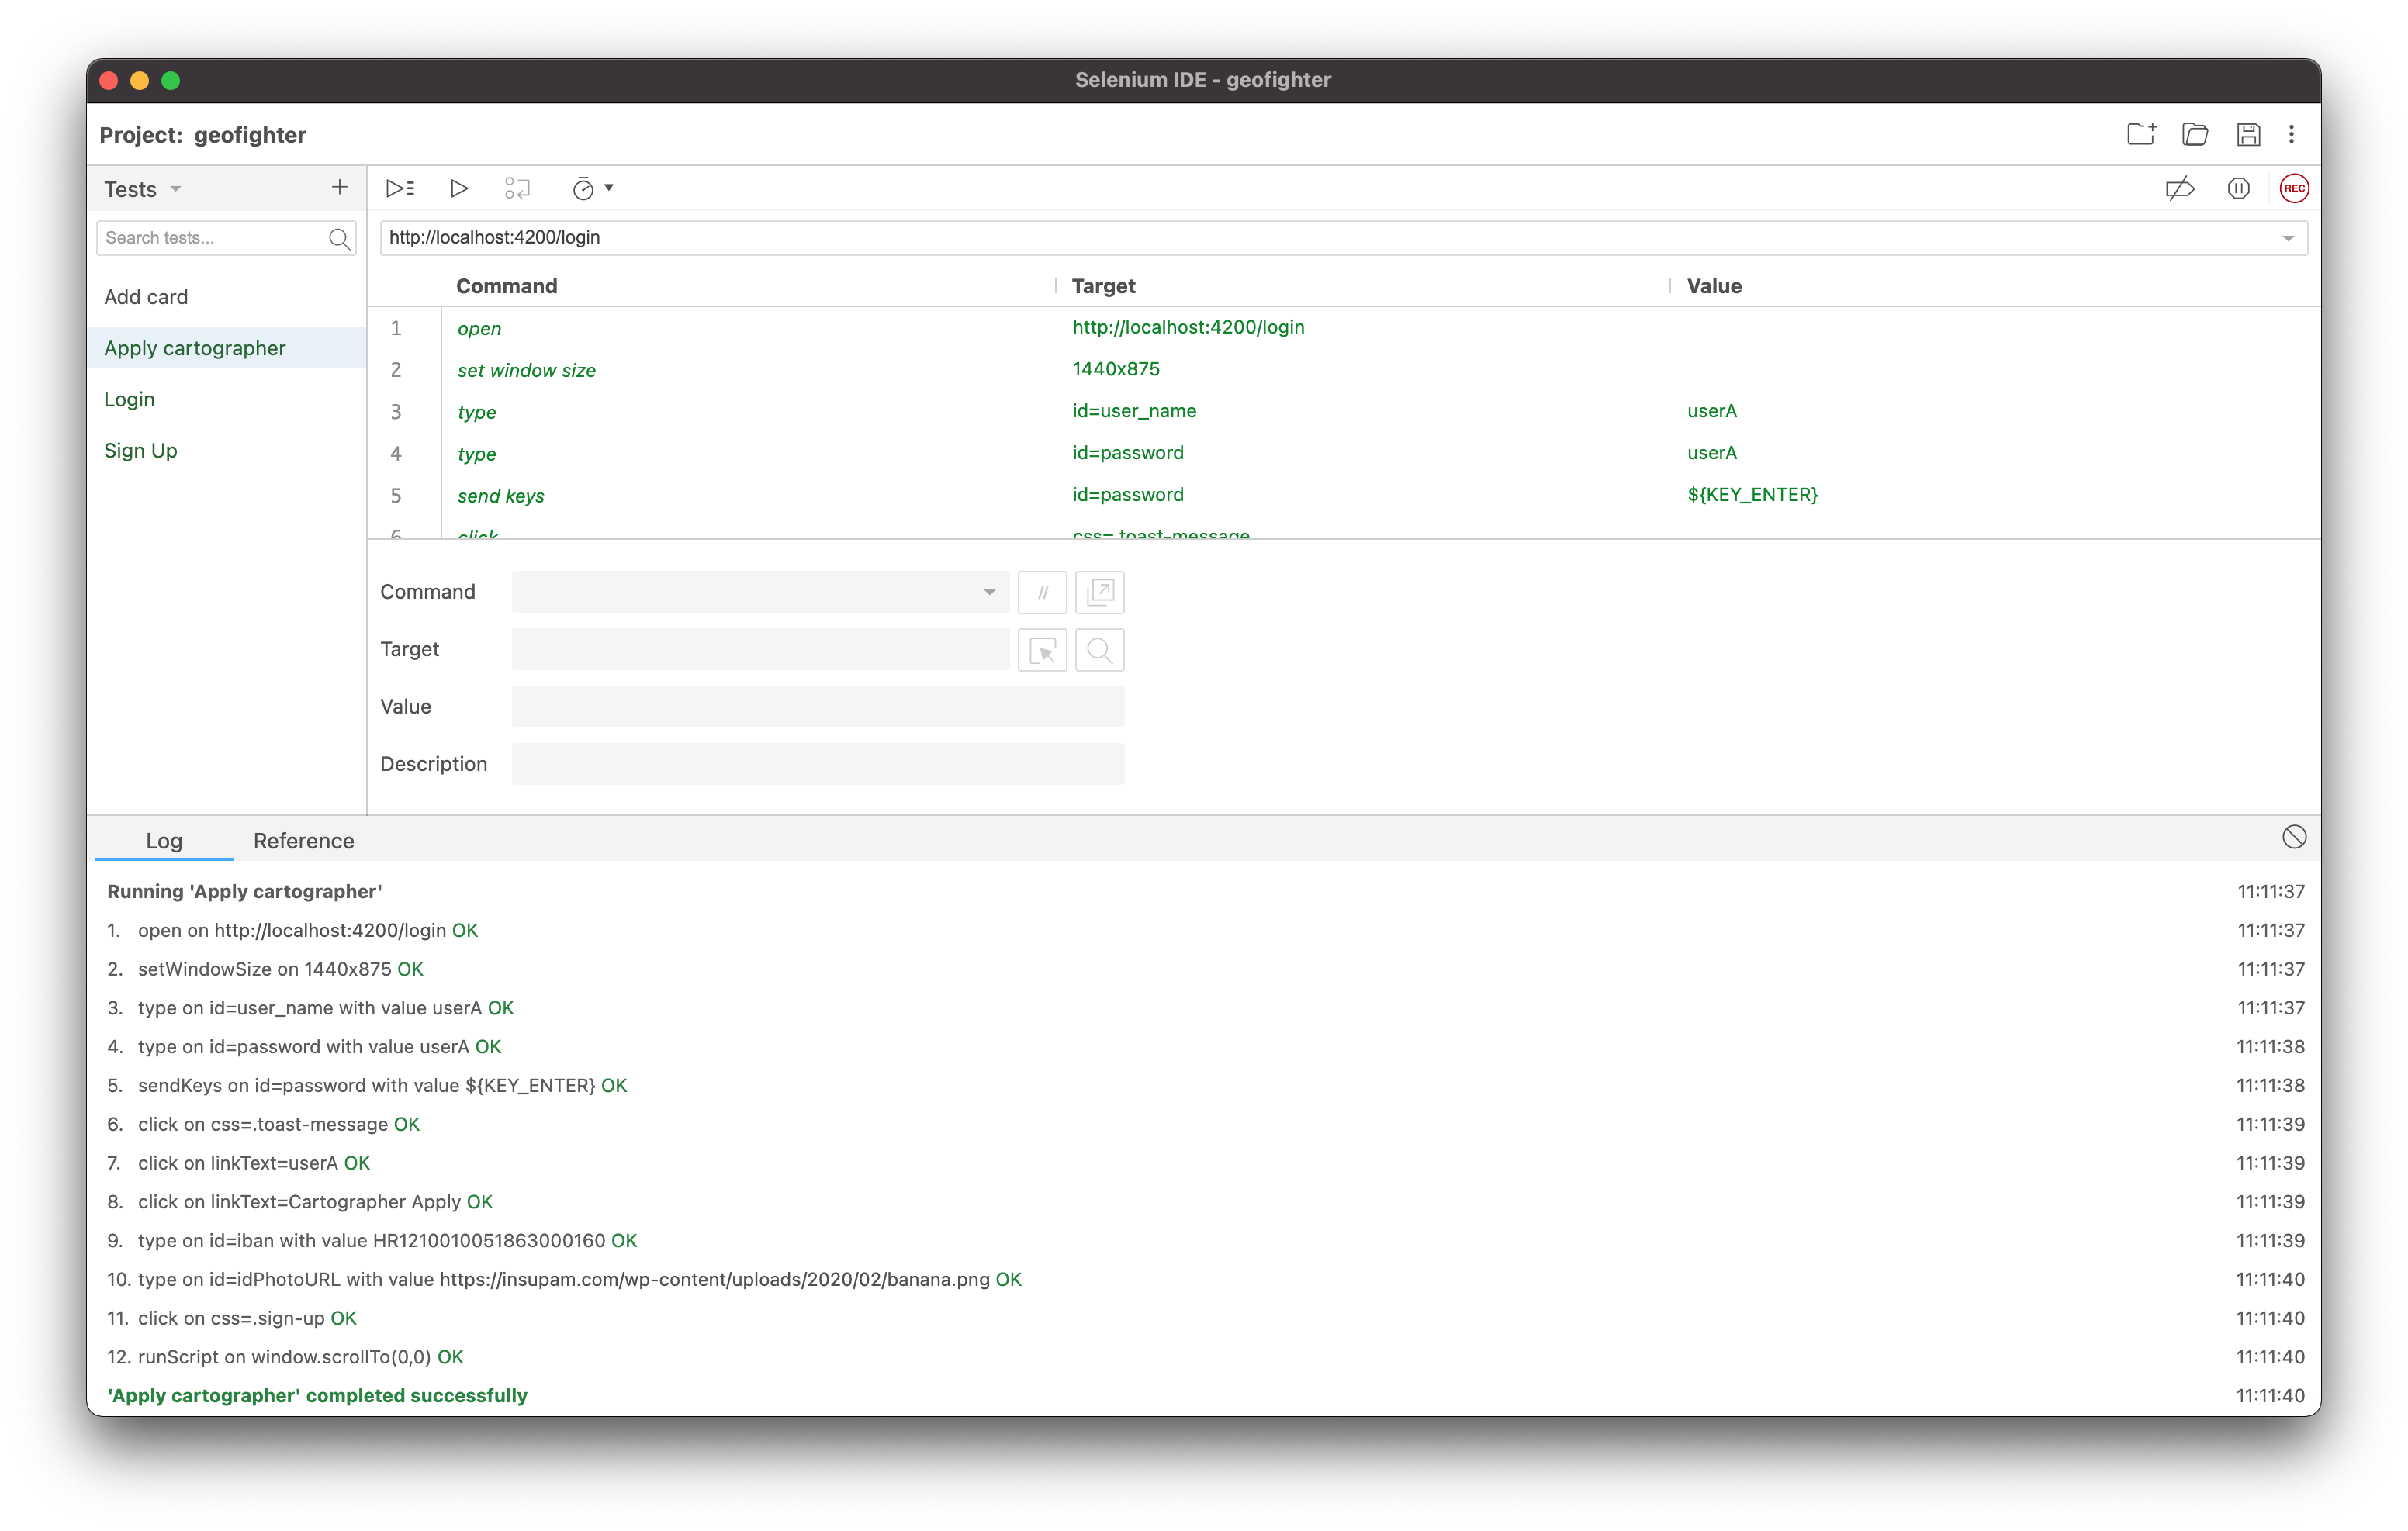
\includegraphics[scale=0.27]{slike/SeleniumCartographerTest.png} \\
				\caption{ Selenium test koji prikazuje ispravnu prijavu korisnika za poziciju kartografa}
				\label{fig:SeleniumCartographerTest}
			\end{figure}

			\subsubsection{Test 4: Dodavanje nove karte u sustav}
			\textbf{Očekivano: } Nakon uspješne prijave korisnika u aplikaciju i nakon što korisnik stisne gumb \textit{Create new card} učitava se stranica s formom za unos podataka potrebnih za dodavanje nove karte u sustav: \textit{naziv, opis, poveznica na sliku lokacije} i vrijednost za 3 parametra jačine karte:  \textit{dostupnost, popularnost, rijetkost}.\\
			\textbf{Rezultat: } Korisnik  je uspješno dodao prijavu za novu kartu ili  je  sustav  dojavio grešku.\\

			\begin{figure}[H]
				\centering
				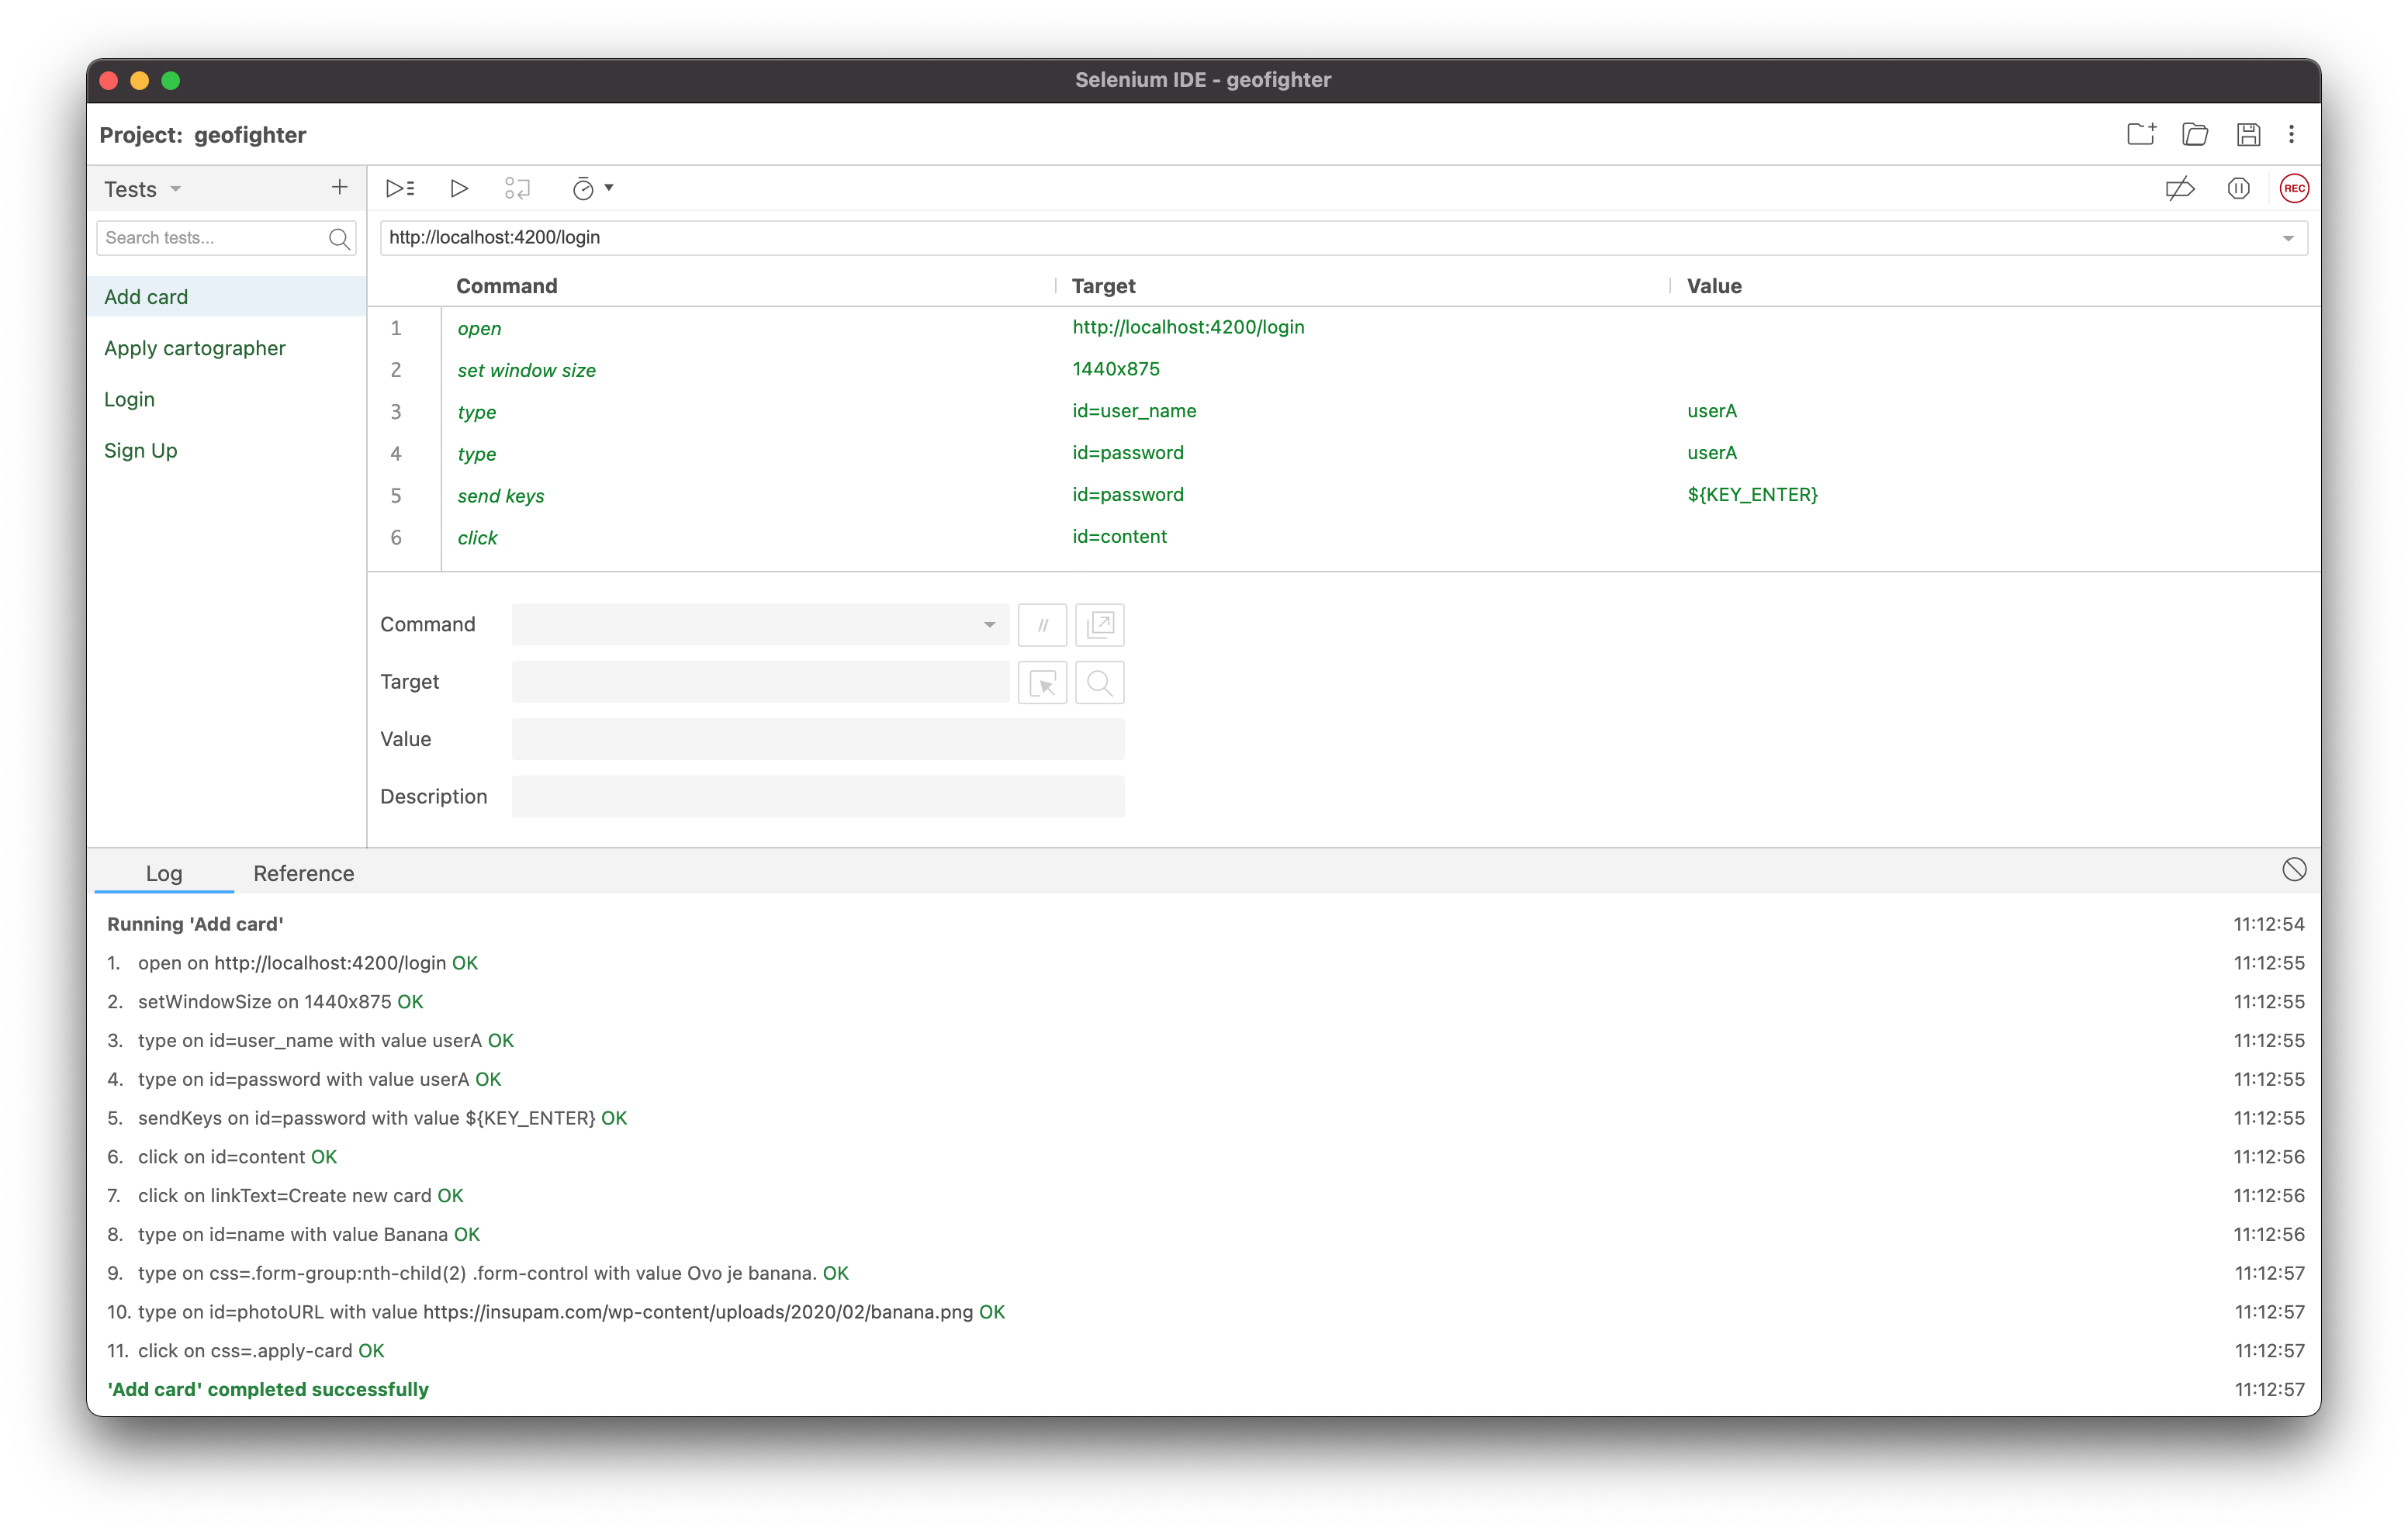
\includegraphics[scale=0.27]{slike/SeleniumCardSuccess.png} \\
				\caption{ Selenium test koji prikazuje ispravno dodavanje karte u sustav}
				\label{fig:SeleniumCartographerSuccess}
			\end{figure}

		    \eject
		
		
		\section{Dijagram razmještaja}
			
			 \textnormal{Dijagram razmještaja opisuje topologiju sklopovlja i programsku potporu koja se koristi u implementaciji sustava u njegovom radnom okruženju. Komponente programske potpore deployane su na oblak platformu Heroku. Heroku je platforma (PaaS) koja razvojnim programerima omogućuje izgradnju, pokretanje i upravljanje aplikacijama u potpunosti u oblaku. Sustav je baziran na arhitekturi klijent - poslužitelj. Komunikacija između njih odvija se HTTP protokolom.}
			
			
			\begin{figure}[H]
				\centering
				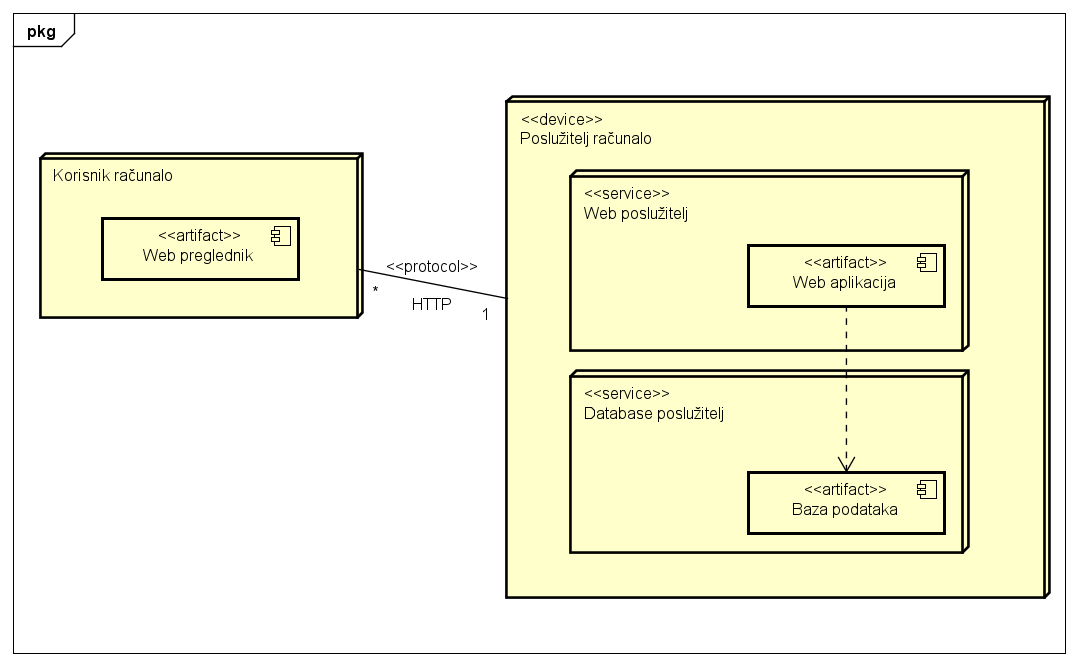
\includegraphics[scale=0.58]{dijagrami/Deployment Diagram0} \\
				\caption{Dijagram razmještaja}
				\label{fig:UC8_sekvencijski}
			\end{figure}
		
			\eject
		
		\section{Upute za puštanje u pogon}
		
			\textit{Za puštanje u pogon GeoFighter aplikacije iz izvornog kôda potrebno je nekoliko preduvjeta: \textbf{PostgreSQL13, JDK11 i Node.js 15}. Uz sve te aplikacije skinute i instalirane lako je kompajlirati i aplikaciju pokrenuti na vlastitom računalu. Aplikacija je također pokrenuta na javno dostupnom poslužitelju \textbf{Heroku} o čemu piše više u nastavku.\\}
			
			\textbf{\textit{Koraci za pokretanje na lokalnom računalu:}}
			
			\begin{itemize}
				
				\item U PostgreSQL DBMSu stvoriti novu bazu podataka te zapisati njeno ime(baze podataka) uz ime korisnika-vlasnika baze podataka, njegove šifre i portu baze.
				
				\item Unutar root direktorija otvoriti datoteku čiji je path\\ \textit{/izvorniKod/geoFighterSpring/src/main/resources/application-local.properties}\\ i unutar nje promijeniti sljedeće parametre: \begin{packed_enum}
					
					\item \textit{spring.datasource} parametre s parametrima novo-kreirane baze podataka. (Voditi brigu o portu, imenu baze podataka, te korisničkom imenu i lozinci vlasnika te baze)
					
					\item \textit{spring.mail} parametre s parametrima željenog mail servisa kako bi se mogli slati mailovi potvrde. (mail servis može biti javan kao što je trenutni \textit{gmail}, a moguće je koristiti testni kao što je \textit{mailtrap}\\ \url{https://mailtrap.io})
				\end{packed_enum}
			
				\begin{figure}[H]
					\centering
					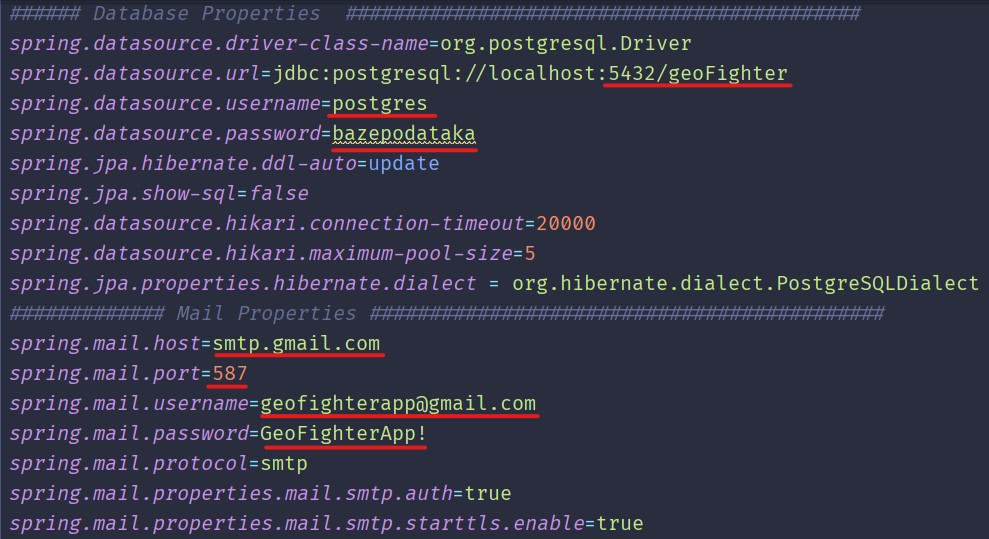
\includegraphics[scale=0.4]{slike/Properties} \\%veličina u odnosu na širinu linije
					\caption{Što promijeniti u application-local.properties}
					\label{fig:properties} %label mora biti drugaciji za svaku sliku
				\end{figure}
			
				
				\item Otvoriti konzolu i pozicionirati se unutar \textit{/izvorniKod/geoFighterSpring/} i pokrenuti naredbu \textit{"./gradlew bootRun -Dspring.profiles.active=local"} s kojom se izkompajlira i pokrene backend servis.
				
				\item Otvoriti drugu konzolu i pozicionirati se unutar \textit{/izvorniKod/angular-geofighter/} i pokrenuti naredbu \textit{"npm install"} s kojom se instaliraju sve potrebno za frontend servis. Zatim pokrenuti naredbu \textit{"ng build"}, te na kraju \textit{"npm start"} kojim se pokreće frontend servis na portu 4200.
				
				\item Ako su pokrenuti backend i frontend servis i ne javlju se greške u konzoli, aplikacija je spremna za korištenje na lokalnom računalu.\\\\
				
			\end{itemize}
		
			
			\textit{Aplikacija je puštena u pogon na javno dostupnom poslužitelju \textbf{Heroku} tako da su sve tri komponente (DB, FrontEnd i BackEnd) tamo pokrenute i moguće joj je pristupiti s linka:}\\
			\url{https://angularfrontend-release.herokuapp.com/}\\
						
			\textit{GitLab repozitorij \url{https://gitlab.com/MatejC_FER/pi} također sadrži CI/CD (Continuous integration and continuous delivery) implementiran pomoću kojeg se pri svakom commitu na \textbf{Master} branch automatski aplikacija izgradila i deployala na \textbf{Heroku} javni poslužitelj. Tako nije potrebno lokalno pokretati aplikaciju nakon izmjena, već je dovoljno na repozitorij pohraniti primjene.}
			
			
			\eject 
	\chapter{Zaključak i budući rad}
		
		\textnormal{Zadatak našeg projekta bio je razviti web aplikaciju "Geofighter", interaktivnu igru u kojoj korisnici fizički posjećuju lokacije u Hrvatskoj. Igrači dolaze do znamenitosti, ustanova, penju se do planinarskih domova ili istražuju Nacionalne parkove te na svakom cilju imaju priliku sakupiti kartu lokacije. Svaka karta lokacije ima 3 atributa koji određuju njenu vrijednost i upravo ti atributi služe kao materijal za borbu među igračima. Igrači iz svoje zbirke karata lokacija odabiru 3 karte, povežu se s igračem po želji blizu njih i kreću u borbu. Igrač također može unijeti novu lokaciju koja, ako je odobrena od strane kartografa, postaje pristupna svim igračima. Korisnik može imati i ulogu kartografa ili administratora koji imaju dodatne ovlasti.}\\
		 
		 \textnormal{Prva faza projekta bila je detaljno opisati projektni zadatak na čemu je grupa složno radila kako bi svi dijelovi zadatka bili razrađeni i svi članovi grupe detaljno upućeni u posao koji će se obavljati. Nakon razrađenog opisa, također složno napisali smo funkcionalne i ostale zahtjeve po kojima smo se kasnije orijentirali u raspoređivanju posla te pri oblikovanju i opisu arhitekture. Grupa se upoznala međusobno, a komunikaciju smo odlučili izvesti preko platforme Slack gdje je voditelj grupe otvorio kanale za razne dijelove projekta te nam je tamo slao sve obavijesti. Sastanke smo odlučili obavljati online na tjednoj bazi preko platforme Zoom i Teams, a po potrebi imali smo i koji izvanredni sastanak. Svi smo se upoznali s Git-om (i GitLab-om) te Latex-om (i TeXstudio-m). Pred kraj prve faze počeli smo se upoznavati s tehnologijama Java Spring za backend i Angular za frontend te izradili kostur aplikacije. Upoznavanje s tehnologijama oduzelo nam je puno vremena i istraživanja materijala na internetu s obzirom na to da se prije s njima nismo susreli. U zadnja dva tjedna prve faze završili smo početni (ne tako mali) dio backenda te login i signup funkcionalnosti skupa s nekim osnovnim komponentama frontenda.}\\
		 
		 \textnormal{Na početku druge faze uslijedila su 2 tjedna neprestanog programiranja, istraživanja i raznih uspjelih i neuspjelih pokušaja implementacije određenih funkcionalnosti. Grupa se ravnomjerno raspodijelila tako da svaka osoba radi i backend i frontend za njoj dodijeljenu funkcionalnost. Problema je bilo, pogotovo zato što smo se svi prvi puta susreli s ovako velikim projektom koristeći ove (nama nove) tehnologije Java Spring i Angular, ali su svi timskim radom uspješno riješeni. Uz tehničke probleme vezane uz prethodno nepoznavanje tehnologija, važno bi bilo istaknuti da je dokumentacija za leaflet library bila loše napisana za kombinaciju leaflet-routing-machine i typescript, što je u konačnici riješeno uz puno ispravljanja pogrešaka i proučavanja izvora na internetu kao što je Stack Overflow. Nakon ta 2 tjedna 90\% funkcionalnosti je završeno, čime je stvorena alfa inačica projekta. Ostatak druge faze projekta proveli smo dovršavajući i popravljajući funkcionalnosti, radeći na samom fizičkom izgledu aplikacije (engl. user-experience) i testirajući određene funkcionalnosti. Riješili smo probleme koji su se pojavili, dovršavali dokumentaciju i pripremali prezentaciju projekta.}\\
		 
		 \textnormal{Na kraju projekta, cijeli tim vrlo je zadovoljan završnim proizvodom našeg rada. Svi funkcionalni zahtjevi uspješno su implementirani, a izgledom i načinom na koji aplikacija radi u potpunosti smo zadovoljni. Dakako, ostvarenje projekta bilo bi kvalitetnije i brže da su članovi grupe imali više iskustva s tehnologijama koje smo koristili, ali i iskustva u programskom inženjerstvu. Ovaj projekt donio nam je mnoga nova znanja ne samo u podučju raznih tehnologija nego i u području timskog rada te općenito rada na projektima ovakve vrste. To znanje zasigurno će nam koristiti u budućnosti i biti oslonac u daljnjem učenju i usavršavanju pri radu na timskim projektima.}\\
		
		\eject 

	\chapter*{Popis literature}
		\addcontentsline{toc}{chapter}{Popis literature}
	 	
 		\textbf{\textit{Kontinuirano osvježavanje}}
	
		\textit{Popisati sve reference i literaturu koja je pomogla pri ostvarivanju projekta.}
		
		
		\begin{enumerate}
			
			
			\item  Programsko inženjerstvo, FER ZEMRIS, \url{http://www.fer.hr/predmet/proinz}
			
			\item  I. Sommerville, "Software engineering", 8th ed, Addison Wesley, 2007.
			
			\item  T.C.Lethbridge, R.Langaniere, "Object-Oriented Software Engineering", 2nd ed. McGraw-Hill, 2005.
			
			\item  I. Marsic, Software engineering book``, Department of Electrical and Computer Engineering, Rutgers University, \url{http://www.ece.rutgers.edu/~marsic/books/SE}
			
			\item  The Unified Modeling Language, \url{https://www.uml-diagrams.org/}
			
			\item  Astah Community, \url{http://astah.net/editions/uml-new}
		\end{enumerate}
		
		 
	
	
	\begingroup
	\renewcommand*\listfigurename{Indeks slika i dijagrama}
	%\renewcommand*\listtablename{Indeks tablica}
	%\let\clearpage\relax
	\listoffigures
	%\vspace{10mm}
	%\listoftables
	\endgroup
	\addcontentsline{toc}{chapter}{Indeks slika i dijagrama}


	
	\eject 
		
	\chapter*{Dodatak: Prikaz aktivnosti grupe}
		\addcontentsline{toc}{chapter}{Dodatak: Prikaz aktivnosti grupe}
		
		\section*{Dnevnik sastajanja}
		
		\textbf{\textit{Kontinuirano osvježavanje}}\\
		
		 \textit{U ovom dijelu potrebno je redovito osvježavati dnevnik sastajanja prema predlošku.}
		
		\begin{packed_enum}
			\item  sastanak
			
			\item[] \begin{packed_item}
				\item Datum: 6.listopada 2020.
				\item Prisustvovali: M.Čubek, I.Hrastnik, A.Markovinović, A.Papak, J.Štracak, J.Vrhovec
				\item Teme sastanka: Upoznavanje, Dogovor osnova projekta
				\begin{packed_item}
					\item  Upoznavanje članova novog projekta
					\item  Dogovor oko tehnologije i diskusija teme
				\end{packed_item}
			\end{packed_item}
			
			\item  sastanak
			\item[] \begin{packed_item}
				\item Datum: 7. listopada 2020.
				\item Prisustvovali: M.Čubek, I.Hrastnik, A.Markovinović, A.Papak, J.Štracak, J.Vrhovec
				\item Teme sastanka: Diskusija s asistentom
				\begin{packed_item}
					\item  Prvi sastanak s asistentom
					\item  Upoznavanje s predmetom i rokovima za projekt
				\end{packed_item}
			\end{packed_item}
		
			\item  sastanak
			\item[] \begin{packed_item}
				\item Datum: 14. listopada 2020.
				\item Prisustvovali: M.Čubek, I.Hrastnik, A.Markovinović, A.Papak, J.Štracak, J.Vrhovec
				\item Teme sastanka: Latex, raspodjela posla dokumentacije
				\begin{packed_item}
					\item  Demonstracija latex alata
					\item  Raspodjela posla 2. poglavlja među članove
				\end{packed_item}
			\end{packed_item}
		
			\item  sastanak
			\item[] \begin{packed_item}
				\item Datum: 14. listopada 2020.
				\item Prisustvovali: M.Čubek, J.Knežević
				\item Teme sastanka: Dobrodošlica, Dovođenje u tok
				\begin{packed_item}
					\item  Dobrodošlica novoga člana tima
					\item  Upoznavanje člana sa zadatkom i projektnim planom
				\end{packed_item}
			\end{packed_item}
		
			\item  sastanak
			\item[] \begin{packed_item}
				\item Datum: 20. listopada 2020.
				\item Prisustvovali: M.Čubek, J.Knežević, I.Hrastnik, A.Markovinović, A.Papak, J.Štracak, J.Vrhovec
				\item Teme sastanka: 2 poglavlje recap, dogovor za 3. poglavlje, pitanja za asistenta
				\begin{packed_item}
					\item  Pregled napisanog za 2. poglavlje i diskusija
					\item  Dogovor poslova za 3. poglavlje
					\item  Formuliranje pitanja za asistenta u terminu labosa
				\end{packed_item}
			\end{packed_item}
		
			\item  sastanak
			\item[] \begin{packed_item}
				\item Datum: 22. listopada 2020.
				\item Prisustvovali: M.Čubek, J.Knežević, I.Hrastnik, A.Markovinović, A.Papak, J.Štracak, J.Vrhovec, H. Nuić
				\item Teme sastanka: 3. Lab, Igra karata, 3 poglavlje
				\begin{packed_item}
					\item 3. laboratorijska vježba s asistentom, pitanja
					\item Dogovor detalja oko igre i bodovanja karata
					\item 3. Poglavlje, razrada obrazaca uporabe i podjela posla
				\end{packed_item}
			\end{packed_item}
		
			\item  sastanak
			\item[] \begin{packed_item}
				\item Datum: 28. listopada 2020.
				\item Prisustvovali: M.Čubek, J.Knežević, I.Hrastnik, A.Markovinović, A.Papak, J.Štracak, J.Vrhovec
				\item Teme sastanka: 3. poglavlje pregled, Dogovor o učenju tehnologija, Preference tehnologije
				\begin{packed_item}
					\item Pregled do sada odrađenog iz 3. poglavlja
					\item Brzi prolaz kroz materijale za učenje tehnologija Angular i Spring Boot
					\item Raspodjela članova tima na tehnologiju koja ih više zanima
				\end{packed_item}
			\end{packed_item}
		
			\item  sastanak
			\item[] \begin{packed_item}
				\item Datum: 29. listopada 2020.
				\item Prisustvovali: M.Čubek, J.Knežević, I.Hrastnik, A.Papak, J.Štracak, J.Vrhovec, H. Nuić
				\item Teme sastanka: Pregled točnosti 3. poglavlja, Zadavanje sekvencijskog dijagrama
				\begin{packed_item}
					\item Brzi pregled napisanog 3. poglavlja i pregled grešaka u njemu
					\item Zadavanje obrazaca uporabe koje treba pretvoriti u sekvencijski dijagram
				\end{packed_item}
			\end{packed_item}
		
			\item  sastanak
			\item[] \begin{packed_item}
				\item Datum: 3. studenoga 2020.
				\item Prisustvovali: M.Čubek, J.Knežević, I.Hrastnik, A.Papak, J.Štracak, J.Vrhovec, H. Nuić
				\item Teme sastanka: Pregled implementacijskih detalja, dogovor frontenda
				\begin{packed_item}
					\item Pregled napisanog Spring backenda
					\item Dogovaranje detalja za implementaciju Angular frontenda
				\end{packed_item}
			\end{packed_item}
		
			\item  sastanak
			\item[] \begin{packed_item}
				\item Datum: 10. studenoga 2020.
				\item Prisustvovali: M.Čubek, J.Knežević, I.Hrastnik, A.Papak, J.Štracak, J.Vrhovec, H. Nuić
				\item Teme sastanka: Pregled generičkih funkcionalnosti
				\begin{packed_item}
					\item Pregled rada login i register funkcionalnosti za korisnika u cjelini
					\item Dogovor implementacije login i register funkcionalnosti za kartografa i administratora
				\end{packed_item}
			\end{packed_item}
		
			\item  sastanak
			\item[] \begin{packed_item}
				\item Datum: 27. studenoga 2020.
				\item Prisustvovali: M.Čubek, J.Knežević, I.Hrastnik, A.Papak, J.Štracak, J.Vrhovec
				\item Teme sastanka: Dogovor o daljnjem razvoju, pregled odrađenog posla
				\begin{packed_item}
					\item Pregled dolazećih zadataka
					\item Pregled odrađenih zadataka
					\item Diskusija o daljnjem razvoju
					\item Prijedlozi i ideje
				\end{packed_item}
			\end{packed_item}
		
			\item  sastanak
			\item[] \begin{packed_item}
				\item Datum: 8. prosinac 2020.
				\item Prisustvovali: M.Čubek, I.Hrastnik, A.Papak, J.Štracak, J.Vrhovec, A.Markovinović
				\item Teme sastanka: Podjela zadataka za alfa verziju aplikacije
				\begin{packed_item}
					\item Podjela zadataka za alfa verziju
					\item Prijedlozi za alfa verziju
					\item Zadavanje zadataka i rokova svakom članu
					\item
				\end{packed_item}
			\end{packed_item}
			
			\item  sastanak
			\item[] \begin{packed_item}
				\item Datum: 15. prosinac 2020.
				\item Prisustvovali: M.Čubek, I.Hrastnik, A.Papak, J.Vrhovec, A.Markovinović
				\item Teme sastanka: Rješavanje bugova, diskusija o problemima
				\begin{packed_item}
					\item Pregled odrađenih zadataka za alfa verziju
					\item Pregled problema zadataka i diskusija o rješenjima
					\item Novi zadaci i rokovi dani
				\end{packed_item}
			\end{packed_item}
			
			\item  sastanak
			\item[] \begin{packed_item}
				\item Datum: 17. prosinac 2020.
				\item Prisustvovali: M.Čubek, J.Knežević, I.Hrastnik, A.Papak,  J.Vrhovec, A.Markovinović
				\item Teme sastanka: Rješavanje bugova, dogovor oko dizajna i logike aplikacije
				\begin{packed_item}
					\item Rješavanje bugova i problema
					\item Diskusija oko dizajna aplikacije
					\item Diskusija oko logike aplikacije
				\end{packed_item}
			\end{packed_item}
		
			\item  sastanak
			\item[] \begin{packed_item}
				\item Datum: 20. prosinac 2020.
				\item Prisustvovali: M.Čubek, J.Knežević, I.Hrastnik, A.Papak,  J.Vrhovec, A.Markovinović
				\item Teme sastanka: Probna demonstracija prije alfa predaje zadatka
				\begin{packed_item}
					\item Diskusija oko dizajna i funkcionalnosti
					\item Podjela zadnjih poslova prije alfa predaje
				\end{packed_item}
			\end{packed_item}
		
			\item  sastanak
			\item[] \begin{packed_item}
				\item Datum: 23. prosinac 2020.
				\item Prisustvovali: M.Čubek, J.Knežević, I.Hrastnik, A.Papak,  J.Vrhovec, A.Markovinović, J. Štracak, H. Nuić
				\item Predaja i demonstracija alfa verzije web aplikacije
				\begin{packed_item}
					\item Testiranje web aplikacije
					\item Razgovor o izrađenim dijelovima web aplikacije
					\item Razgovor o dijelovima web aplikacije koji se još moraju napraviti
					\item Rasprava o težini gradiva koje je bilo potrebno shvatiti za izradu
				\end{packed_item}
			\end{packed_item}
		
			\item  sastanak
			\item[] \begin{packed_item}
				\item Datum: 12. siječnja 2021.
				\item Prisustvovali: M.Čubek, J.Knežević, I.Hrastnik, A.Papak,  J.Vrhovec, A.Markovinović, J. Štracak, H. Nuić
				\item Finalne diskusije o završnim radnjama na projektu i razgovor s asistentom.
				\begin{packed_item}
					\item Rasprava o završnim dijagramima.
					\item Pregled napravljenoga.
					\item Upiti asistentu o ispravnosti dijagrama.
					\item Q/A među timom.
				\end{packed_item}
			\end{packed_item}
						
			%
			
		\end{packed_enum}
		
		\eject
		\section*{Tablica aktivnosti}
		
			\textbf{\textit{Kontinuirano osvježavanje}}\\
			
			 \textit{Napomena: Doprinose u aktivnostima treba navesti u satima po članovima grupe po aktivnosti.}
					
						
			
			\begin{longtabu} to \textwidth {|X[7, l]|X[1, c]|X[1, c]|X[1, c]|X[1, c]|X[1, c]|X[1, c]|X[1, c]|}
								
				\cline{2-8} \multicolumn{1}{c|}{\textbf{}} &     \multicolumn{1}{c|}{\rotatebox{90}{\textbf{Matej Čubek }}} & \multicolumn{1}{c|}{\rotatebox{90}{\textbf{Iva Hrastnik }}} &
				\multicolumn{1}{c|}{\rotatebox{90}{\textbf{Jakov Knežević }}} &	\multicolumn{1}{c|}{\rotatebox{90}{\textbf{Anamarija Markovinović }}} &	\multicolumn{1}{c|}{\rotatebox{90}{\textbf{Alen Papak }}} &
				\multicolumn{1}{c|}{\rotatebox{90}{\textbf{Jakov Štracak }}} &
				\multicolumn{1}{c|}{\rotatebox{90}{\textbf{Jakov Vrhovec }}} \\ \hline 
				\endfirsthead
				
			
				\cline{2-8} \multicolumn{1}{c|}{\textbf{}} &     \multicolumn{1}{c|}{\rotatebox{90}{\textbf{Matej Čubek }}} & \multicolumn{1}{c|}{\rotatebox{90}{\textbf{Iva Hrastnik }}} &
				\multicolumn{1}{c|}{\rotatebox{90}{\textbf{Jakov Knežević }}} &	\multicolumn{1}{c|}{\rotatebox{90}{\textbf{Anamarija Markovinović }}} &	\multicolumn{1}{c|}{\rotatebox{90}{\textbf{Alen Papak }}} &
				\multicolumn{1}{c|}{\rotatebox{90}{\textbf{Jakov Štracak }}} &
				\multicolumn{1}{c|}{\rotatebox{90}{\textbf{Jakov Vrhovec }}} \\ \hline  
				\endhead
				
				
				\endfoot
							
				 
				\endlastfoot
				
				Upravljanje projektom 		&8  &  &  &  &  &  &1   \\ \hline
				Opis projektnog zadatka 	&1  &2  &1  &2  &1  &1  &3   \\ \hline
				
				Funkcionalni zahtjevi       &1  &1  &  &2  &  &1  &2    \\ \hline
				Opis pojedinih obrazaca 	&  &  &4  &3  &3  &  &3    \\ \hline
				Dijagram obrazaca 			&  &  &2  &  &  &2  &1    \\ \hline
				Sekvencijski dijagrami 		&  &2  &  &  &  &2  &2    \\ \hline
				Opis ostalih zahtjeva 		&  &0.5  &  &  &  &  &1    \\ \hline

				Arhitektura i dizajn sustava	 &  &  &  &5  &2  &  &1    \\ \hline
				Baza podataka				&1  &  &  &6  &  &  &     \\ \hline
				Dijagram razreda 			&  &  &  &8  &2  &  &2     \\ \hline
				Dijagram stanja				&  &  &  &  &  &1  &1    \\ \hline
				Dijagram aktivnosti 		&  &  &  &  &  &  &1    \\ \hline
				Dijagram komponenti			&  &  &  &  &  &  &1    \\ \hline
				Korištene tehnologije i alati 		&2  &  &  &  &  &  &    \\ \hline
				Ispitivanje programskog rješenja 	&1  &  &  &  &1  &  &    \\ \hline
				Dijagram razmještaja			&  &  &  &  &  &  &1    \\ \hline
				Upute za puštanje u pogon 		&2  &  &  &  &  &  &    \\ \hline 
				Dnevnik sastajanja 			&1  &0.5  &  &  &  &  &4    \\ \hline
				Zaključak i budući rad 		&  &2  &  &  &  &  &    \\  \hline
				Popis literature 			&  &  &  &2  &  &  &    \\  \hline
				
				\textit{CI/CD implementacija} 			&4  &  &  &  &  &  &    \\ \hline
				\textit{Enviroment varijable za deployment} 			&3  &  &  &  &  &3  &    \\ \hline
				\textit{Postavljanje hosting servisa} 			&2  &  &  &  &  &  &    \\ \hline
				\textit{Email template} 			&  &  &2  &  &  &  &    \\ \hline
				\textit{Rad s bazom podataka} 		 			&4  &  &  &2  &6  &  &   \\ \hline 
				\textit{Angular bez UX Dev} 							&17  &5  &3  &26  &  &1  &20    \\ \hline
				\textit{Angular UX Dev} 							&4  &20  &5  &4  &13  &1  &5    \\ \hline
				\textit{Java Spring Dev} 							&35  &6  &13  &18  &24  &  &10   \\  \hline
				\textit{Deployment}						&3  &  &  &  &  &  &  \\  \hline
				\textit{JUnit i Selenium Testing}						&4  &  &4  &  &4  &  &  \\  \hline
				
				
			\end{longtabu}
					
					
		\eject
		\section*{Dijagrami pregleda promjena}
		
		\textbf{\textit{dio 2. revizije}}\\
		
		\textit{Prenijeti dijagram pregleda promjena nad datotekama projekta. Potrebno je na kraju projekta generirane grafove s gitlaba prenijeti u ovo poglavlje dokumentacije. Dijagrami za vlastiti projekt se mogu preuzeti s gitlab.com stranice, u izborniku Repository, pritiskom na stavku Contributors.}
		
	



\end{document} %naredbe i tekst nakon ove naredbe ne ulaze u izgrađen dokument 


